\documentclass[]{article}
\usepackage{lmodern}
\usepackage{amssymb,amsmath}
\usepackage{ifxetex,ifluatex}
\usepackage{fixltx2e} % provides \textsubscript
\ifnum 0\ifxetex 1\fi\ifluatex 1\fi=0 % if pdftex
  \usepackage[T1]{fontenc}
  \usepackage[utf8]{inputenc}
\else % if luatex or xelatex
  \ifxetex
    \usepackage{mathspec}
  \else
    \usepackage{fontspec}
  \fi
  \defaultfontfeatures{Ligatures=TeX,Scale=MatchLowercase}
\fi
% use upquote if available, for straight quotes in verbatim environments
\IfFileExists{upquote.sty}{\usepackage{upquote}}{}
% use microtype if available
\IfFileExists{microtype.sty}{%
\usepackage{microtype}
\UseMicrotypeSet[protrusion]{basicmath} % disable protrusion for tt fonts
}{}
\usepackage[margin=1in]{geometry}
\usepackage{hyperref}
\hypersetup{unicode=true,
            pdftitle={Local Policy Recommendations for Crime Reduction},
            pdfauthor={Alexa Bagnard, Joseph Gaustad, Kevin Hartman, Francis Leung; (W203 Wednesday 6:30pm Summer 2019)},
            pdfborder={0 0 0},
            breaklinks=true}
\urlstyle{same}  % don't use monospace font for urls
\usepackage{color}
\usepackage{fancyvrb}
\newcommand{\VerbBar}{|}
\newcommand{\VERB}{\Verb[commandchars=\\\{\}]}
\DefineVerbatimEnvironment{Highlighting}{Verbatim}{commandchars=\\\{\}}
% Add ',fontsize=\small' for more characters per line
\newenvironment{Shaded}{}{}
\newcommand{\AlertTok}[1]{\textcolor[rgb]{1.00,0.00,0.00}{#1}}
\newcommand{\AnnotationTok}[1]{\textcolor[rgb]{0.00,0.50,0.00}{#1}}
\newcommand{\AttributeTok}[1]{#1}
\newcommand{\BaseNTok}[1]{#1}
\newcommand{\BuiltInTok}[1]{#1}
\newcommand{\CharTok}[1]{\textcolor[rgb]{0.00,0.50,0.50}{#1}}
\newcommand{\CommentTok}[1]{\textcolor[rgb]{0.00,0.50,0.00}{#1}}
\newcommand{\CommentVarTok}[1]{\textcolor[rgb]{0.00,0.50,0.00}{#1}}
\newcommand{\ConstantTok}[1]{#1}
\newcommand{\ControlFlowTok}[1]{\textcolor[rgb]{0.00,0.00,1.00}{#1}}
\newcommand{\DataTypeTok}[1]{#1}
\newcommand{\DecValTok}[1]{#1}
\newcommand{\DocumentationTok}[1]{\textcolor[rgb]{0.00,0.50,0.00}{#1}}
\newcommand{\ErrorTok}[1]{\textcolor[rgb]{1.00,0.00,0.00}{\textbf{#1}}}
\newcommand{\ExtensionTok}[1]{#1}
\newcommand{\FloatTok}[1]{#1}
\newcommand{\FunctionTok}[1]{#1}
\newcommand{\ImportTok}[1]{#1}
\newcommand{\InformationTok}[1]{\textcolor[rgb]{0.00,0.50,0.00}{#1}}
\newcommand{\KeywordTok}[1]{\textcolor[rgb]{0.00,0.00,1.00}{#1}}
\newcommand{\NormalTok}[1]{#1}
\newcommand{\OperatorTok}[1]{#1}
\newcommand{\OtherTok}[1]{\textcolor[rgb]{1.00,0.25,0.00}{#1}}
\newcommand{\PreprocessorTok}[1]{\textcolor[rgb]{1.00,0.25,0.00}{#1}}
\newcommand{\RegionMarkerTok}[1]{#1}
\newcommand{\SpecialCharTok}[1]{\textcolor[rgb]{0.00,0.50,0.50}{#1}}
\newcommand{\SpecialStringTok}[1]{\textcolor[rgb]{0.00,0.50,0.50}{#1}}
\newcommand{\StringTok}[1]{\textcolor[rgb]{0.00,0.50,0.50}{#1}}
\newcommand{\VariableTok}[1]{#1}
\newcommand{\VerbatimStringTok}[1]{\textcolor[rgb]{0.00,0.50,0.50}{#1}}
\newcommand{\WarningTok}[1]{\textcolor[rgb]{0.00,0.50,0.00}{\textbf{#1}}}
\usepackage{longtable,booktabs}
\usepackage{graphicx,grffile}
\makeatletter
\def\maxwidth{\ifdim\Gin@nat@width>\linewidth\linewidth\else\Gin@nat@width\fi}
\def\maxheight{\ifdim\Gin@nat@height>\textheight\textheight\else\Gin@nat@height\fi}
\makeatother
% Scale images if necessary, so that they will not overflow the page
% margins by default, and it is still possible to overwrite the defaults
% using explicit options in \includegraphics[width, height, ...]{}
\setkeys{Gin}{width=\maxwidth,height=\maxheight,keepaspectratio}
\IfFileExists{parskip.sty}{%
\usepackage{parskip}
}{% else
\setlength{\parindent}{0pt}
\setlength{\parskip}{6pt plus 2pt minus 1pt}
}
\setlength{\emergencystretch}{3em}  % prevent overfull lines
\providecommand{\tightlist}{%
  \setlength{\itemsep}{0pt}\setlength{\parskip}{0pt}}
\setcounter{secnumdepth}{5}
% Redefines (sub)paragraphs to behave more like sections
\ifx\paragraph\undefined\else
\let\oldparagraph\paragraph
\renewcommand{\paragraph}[1]{\oldparagraph{#1}\mbox{}}
\fi
\ifx\subparagraph\undefined\else
\let\oldsubparagraph\subparagraph
\renewcommand{\subparagraph}[1]{\oldsubparagraph{#1}\mbox{}}
\fi

%%% Use protect on footnotes to avoid problems with footnotes in titles
\let\rmarkdownfootnote\footnote%
\def\footnote{\protect\rmarkdownfootnote}

%%% Change title format to be more compact
\usepackage{titling}

% Create subtitle command for use in maketitle
\providecommand{\subtitle}[1]{
  \posttitle{
    \begin{center}\large#1\end{center}
    }
}

\setlength{\droptitle}{-2em}

  \title{Local Policy Recommendations for Crime Reduction}
    \pretitle{\vspace{\droptitle}\centering\huge}
  \posttitle{\par}
  \subtitle{Final Report}
  \author{Alexa Bagnard, Joseph Gaustad, Kevin Hartman, Francis Leung \\ (W203 Wednesday 6:30pm Summer 2019)}
    \preauthor{\centering\large\emph}
  \postauthor{\par}
      \predate{\centering\large\emph}
  \postdate{\par}
    \date{8/7/2019}

\usepackage{booktabs}
\usepackage{longtable}
\usepackage{array}
\usepackage{multirow}
\usepackage{wrapfig}
\usepackage{float}
\usepackage{colortbl}
\usepackage{pdflscape}
\usepackage{tabu}
\usepackage{threeparttable}
\usepackage{threeparttablex}
\usepackage[normalem]{ulem}
\usepackage{makecell}
\usepackage{xcolor}

\begin{document}
\maketitle
\begin{abstract}
This is our study on crime. Crime does not pay. Lorem ipsum dolor sit
amet, consectetur adipiscing elit, sed do eiusmod tempor incididunt ut
labore et dolore magna aliqua. Ut enim ad minim veniam, quis nostrud
exercitation ullamco laboris nisi ut aliquip ex ea commodo consequat.
Duis aute irure dolor in reprehenderit in voluptate velit esse cillum
dolore eu fugiat nulla pariatur. Excepteur sint occaecat cupidatat non
proident, sunt in culpa qui officia deserunt mollit anim id est laborum.
\end{abstract}

{
\setcounter{tocdepth}{2}
\tableofcontents
}
\hypertarget{introduction}{%
\section{Introduction}\label{introduction}}

\hypertarget{background}{%
\subsection{Background}\label{background}}

In this report, we seek to examine and discuss determinants of crime and
offer recommend actionable policy recommendations for local politicians
running for election at the county level in North Carolina. For our
analysis, we draw on sample data collected from a study by Cornwell and
Trumball, researchers from the University of Georgia and West Virginia
University. Our sample data includes data on crime rates, arrests,
sentences, demographics, local weekly wages, tax revenues and more drawn
from local and federal government data sources. Although the age of the
data may be a potential limitation of our study, we believe the insights
we gather and policy recommendations remain appropriate for local
campaigns today.

Our primary question that will drive our data exploration are to ask
which variables affect crime rate the most.

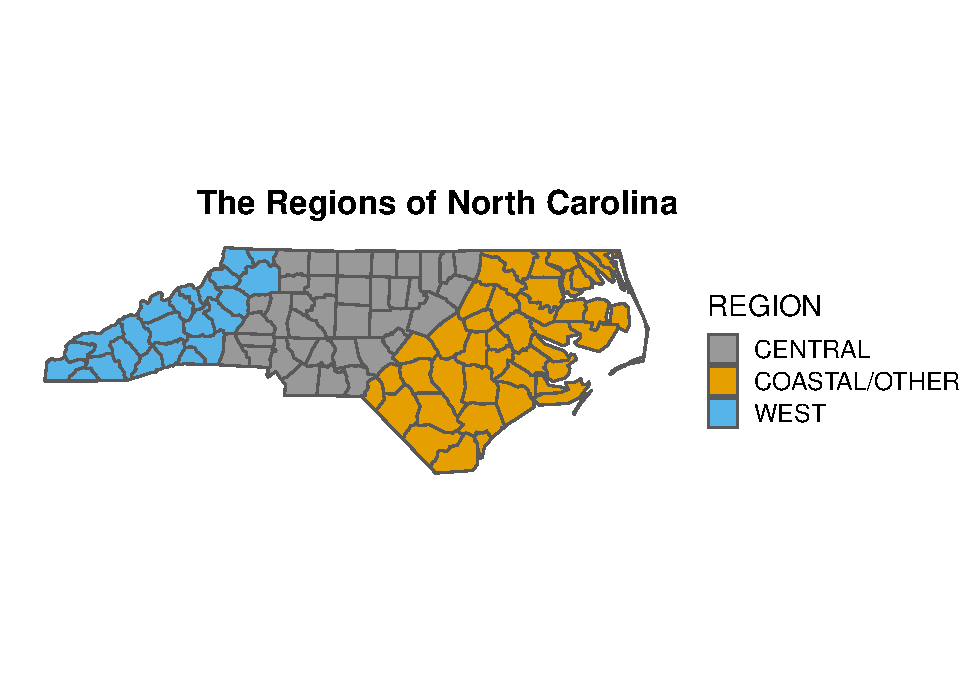
\includegraphics{Bagnard_Gaustad_Hartman_Leung_Lab_3_files/figure-latex/unnamed-chunk-1-1.pdf}

\hypertarget{the-variables}{%
\subsection{The Variables}\label{the-variables}}

The crime\_v2 dataset provided includes 25 variables of interest.

We include them below for reference by category of interest.

\begin{center}
\textbf{Data Dictionary}
\end{center}

\begin{longtable}[]{@{}ll@{}}
\toprule
Category & Variable\tabularnewline
\midrule
\endhead
Crime Rate & crmrte\tabularnewline
Geographic & county, west, central\tabularnewline
Demographic & urban, density, pctmin80, pctymle\tabularnewline
Economic - Wage & wcon, wtuc, wtrd, wfir, wser, wmfg, wfed, wsta,
wloc\tabularnewline
Economic - Revenue & taxpc\tabularnewline
Law Enforcment & polpc, prbarr, prbconv, mix\tabularnewline
Judicial/Sentencing & prbpris, avgsen\tabularnewline
Time Period & year\tabularnewline
\bottomrule
\end{longtable}

\begin{center}
Table 1: Data Dictionary
\end{center}

The variables above operationalize the conditions we wish to explore and
their affects on crime rate

Chiefly, these break down as follows.

\begin{itemize}
\item
  The Economic variables measures the county's economic activity and
  health (e.g.~opportunity to pursue legal forms of income). These
  variables come in the form of available wages and tax revenue returned
  to the county.
\item
  The Law enforcment variables measures the county's ability to utilize
  law enforcment policy to deter crime. Similarly, the Judicial
  variables also signify impact of deterence to crime.
\item
  The Demographic variables measure the cultural variability that
  represent the social differences between each county, such as urban vs
  rural and minority populations.
\item
  The Geographic elements are categorical. They represent they ways in
  which the population is segmented by geography.
\end{itemize}

\hypertarget{exploratory-data-analysis-eda}{%
\section{Exploratory Data Analysis
(EDA)}\label{exploratory-data-analysis-eda}}

\hypertarget{data-prep-and-exploration}{%
\subsection{Data Prep and Exploration}\label{data-prep-and-exploration}}

We begin our analysis by loading the data set and performing basic
checks and inspections.

\begin{Shaded}
\begin{Highlighting}[]
\NormalTok{dfCrime =}\StringTok{ }\KeywordTok{read.csv}\NormalTok{(}\StringTok{"crime_v2.csv"}\NormalTok{)}
\KeywordTok{summary}\NormalTok{(dfCrime)}
\end{Highlighting}
\end{Shaded}

\begin{verbatim}
     county           year        crmrte             prbarr       
 Min.   :  1.0   Min.   :87   Min.   :0.005533   Min.   :0.09277  
 1st Qu.: 52.0   1st Qu.:87   1st Qu.:0.020927   1st Qu.:0.20568  
 Median :105.0   Median :87   Median :0.029986   Median :0.27095  
 Mean   :101.6   Mean   :87   Mean   :0.033400   Mean   :0.29492  
 3rd Qu.:152.0   3rd Qu.:87   3rd Qu.:0.039642   3rd Qu.:0.34438  
 Max.   :197.0   Max.   :87   Max.   :0.098966   Max.   :1.09091  
 NA's   :6       NA's   :6    NA's   :6          NA's   :6        
        prbconv      prbpris           avgsen           polpc         
            : 5   Min.   :0.1500   Min.   : 5.380   Min.   :0.000746  
 0.588859022: 2   1st Qu.:0.3648   1st Qu.: 7.340   1st Qu.:0.001231  
 `          : 1   Median :0.4234   Median : 9.100   Median :0.001485  
 0.068376102: 1   Mean   :0.4108   Mean   : 9.647   Mean   :0.001702  
 0.140350997: 1   3rd Qu.:0.4568   3rd Qu.:11.420   3rd Qu.:0.001877  
 0.154451996: 1   Max.   :0.6000   Max.   :20.700   Max.   :0.009054  
 (Other)    :86   NA's   :6        NA's   :6        NA's   :6         
    density            taxpc             west           central      
 Min.   :0.00002   Min.   : 25.69   Min.   :0.0000   Min.   :0.0000  
 1st Qu.:0.54741   1st Qu.: 30.66   1st Qu.:0.0000   1st Qu.:0.0000  
 Median :0.96226   Median : 34.87   Median :0.0000   Median :0.0000  
 Mean   :1.42884   Mean   : 38.06   Mean   :0.2527   Mean   :0.3736  
 3rd Qu.:1.56824   3rd Qu.: 40.95   3rd Qu.:0.5000   3rd Qu.:1.0000  
 Max.   :8.82765   Max.   :119.76   Max.   :1.0000   Max.   :1.0000  
 NA's   :6         NA's   :6        NA's   :6        NA's   :6       
     urban            pctmin80           wcon            wtuc      
 Min.   :0.00000   Min.   : 1.284   Min.   :193.6   Min.   :187.6  
 1st Qu.:0.00000   1st Qu.: 9.845   1st Qu.:250.8   1st Qu.:374.6  
 Median :0.00000   Median :24.312   Median :281.4   Median :406.5  
 Mean   :0.08791   Mean   :25.495   Mean   :285.4   Mean   :411.7  
 3rd Qu.:0.00000   3rd Qu.:38.142   3rd Qu.:314.8   3rd Qu.:443.4  
 Max.   :1.00000   Max.   :64.348   Max.   :436.8   Max.   :613.2  
 NA's   :6         NA's   :6        NA's   :6       NA's   :6      
      wtrd            wfir            wser             wmfg      
 Min.   :154.2   Min.   :170.9   Min.   : 133.0   Min.   :157.4  
 1st Qu.:190.9   1st Qu.:286.5   1st Qu.: 229.7   1st Qu.:288.9  
 Median :203.0   Median :317.3   Median : 253.2   Median :320.2  
 Mean   :211.6   Mean   :322.1   Mean   : 275.6   Mean   :335.6  
 3rd Qu.:225.1   3rd Qu.:345.4   3rd Qu.: 280.5   3rd Qu.:359.6  
 Max.   :354.7   Max.   :509.5   Max.   :2177.1   Max.   :646.9  
 NA's   :6       NA's   :6       NA's   :6        NA's   :6      
      wfed            wsta            wloc            mix         
 Min.   :326.1   Min.   :258.3   Min.   :239.2   Min.   :0.01961  
 1st Qu.:400.2   1st Qu.:329.3   1st Qu.:297.3   1st Qu.:0.08074  
 Median :449.8   Median :357.7   Median :308.1   Median :0.10186  
 Mean   :442.9   Mean   :357.5   Mean   :312.7   Mean   :0.12884  
 3rd Qu.:478.0   3rd Qu.:382.6   3rd Qu.:329.2   3rd Qu.:0.15175  
 Max.   :598.0   Max.   :499.6   Max.   :388.1   Max.   :0.46512  
 NA's   :6       NA's   :6       NA's   :6       NA's   :6        
    pctymle       
 Min.   :0.06216  
 1st Qu.:0.07443  
 Median :0.07771  
 Mean   :0.08396  
 3rd Qu.:0.08350  
 Max.   :0.24871  
 NA's   :6        
\end{verbatim}

First, we will remove the missing rows from the dataset.

\begin{Shaded}
\begin{Highlighting}[]
\KeywordTok{nrow}\NormalTok{(dfCrime)}
\end{Highlighting}
\end{Shaded}

\begin{verbatim}
[1] 97
\end{verbatim}

\begin{Shaded}
\begin{Highlighting}[]
\NormalTok{dfCrime <-}\KeywordTok{na.omit}\NormalTok{(dfCrime) }\CommentTok{# omit the NA rows}
\KeywordTok{nrow}\NormalTok{(dfCrime)}
\end{Highlighting}
\end{Shaded}

\begin{verbatim}
[1] 91
\end{verbatim}

Next, we will inspect the data to see if there are duplicate records

\begin{Shaded}
\begin{Highlighting}[]
\NormalTok{dfCrime[}\KeywordTok{duplicated}\NormalTok{(dfCrime),]}
\end{Highlighting}
\end{Shaded}

\begin{verbatim}
   county year    crmrte   prbarr     prbconv  prbpris avgsen      polpc
89    193   87 0.0235277 0.266055 0.588859022 0.423423   5.86 0.00117887
     density    taxpc west central urban pctmin80     wcon     wtuc
89 0.8138298 28.51783    1       0     0  5.93109 285.8289 480.1948
       wtrd     wfir     wser   wmfg   wfed   wsta   wloc       mix
89 268.3836 365.0196 295.9352 295.63 468.26 337.88 348.74 0.1105016
      pctymle
89 0.07819394
\end{verbatim}

A duplicate row exists. We'll remove it.

\begin{Shaded}
\begin{Highlighting}[]
\NormalTok{dfCrime <-}\StringTok{ }\NormalTok{dfCrime[}\OperatorTok{!}\KeywordTok{duplicated}\NormalTok{(dfCrime),] }\CommentTok{# remove the duplicated row}
\end{Highlighting}
\end{Shaded}

We also saw that pbconv was coded as a level. It is not a level but a
ratio. We'll change that now.

\begin{Shaded}
\begin{Highlighting}[]
\NormalTok{dfCrime}\OperatorTok{$}\NormalTok{prbconv<-}\KeywordTok{as.numeric}\NormalTok{(}\KeywordTok{levels}\NormalTok{(dfCrime}\OperatorTok{$}\NormalTok{prbconv))[dfCrime}\OperatorTok{$}\NormalTok{prbconv]}
\end{Highlighting}
\end{Shaded}

We also notice by comparision of pctymle and pctmin80 one of the
variables is off by a factor of 100. We will divide pctmin80 by 100 so
the two variables are in the same unit terms.

\begin{Shaded}
\begin{Highlighting}[]
\NormalTok{dfCrime}\OperatorTok{$}\NormalTok{pctmin80<-dfCrime}\OperatorTok{$}\NormalTok{pctmin80}\OperatorTok{/}\DecValTok{100}
\end{Highlighting}
\end{Shaded}

County was expressed as a number. However, it is a categorical variable
and we will convert it to a factor instead.

\begin{Shaded}
\begin{Highlighting}[]
\NormalTok{dfCrime}\OperatorTok{$}\NormalTok{county<-}\KeywordTok{as.factor}\NormalTok{(dfCrime}\OperatorTok{$}\NormalTok{county)}
\end{Highlighting}
\end{Shaded}

Next we inspect the indicator variables to see if they were coded
correctly.

\begin{Shaded}
\begin{Highlighting}[]
\NormalTok{dfCrime }\OperatorTok\StringTok{ }\KeywordTok{group_by}\NormalTok{(west, central) }\OperatorTok\StringTok{ }\KeywordTok{tally}\NormalTok{()}
\end{Highlighting}
\end{Shaded}

\begin{verbatim}
# A tibble: 4 x 3
# Groups:   west [2]
   west central     n
  <int>   <int> <int>
1     0       0    35
2     0       1    33
3     1       0    21
4     1       1     1
\end{verbatim}

\begin{Shaded}
\begin{Highlighting}[]
\NormalTok{dfCrime }\OperatorTok
\KeywordTok{filter}\NormalTok{(west }\OperatorTok{==}\DecValTok{1} \OperatorTok{&}\StringTok{ }\NormalTok{central }\OperatorTok{==}\DecValTok{1}\NormalTok{)}
\end{Highlighting}
\end{Shaded}

\begin{verbatim}
  county year    crmrte   prbarr prbconv  prbpris avgsen      polpc
1     71   87 0.0544061 0.243119 0.22959 0.379175  11.29 0.00207028
   density    taxpc west central urban pctmin80     wcon     wtuc     wtrd
1 4.834734 31.53658    1       1     0  0.13315 291.4508 595.3719 240.3673
      wfir     wser   wmfg   wfed   wsta   wloc       mix    pctymle
1 348.0254 295.2301 358.95 509.43 359.11 339.58 0.1018608 0.07939028
\end{verbatim}

One county was either mis-coded (with west=1 and central=1), or it truly
belongs to both regions. However, this is very unlikely as the proper
coding technique is to widen the data and introduce indicator variables
for each category. It is not likley that data was captured for both
categories.

We will need further analysis on this datapoint to assess proper
treatment options.

For now, we will encode a new region variable and place the datapoint in
its own category.

\begin{Shaded}
\begin{Highlighting}[]
\CommentTok{#Map central and west to a region code, and create a new category for other}
\CommentTok{# Note that county 71 has both western and central codes}
\NormalTok{dfCrime}\OperatorTok{$}\NormalTok{region <-}\StringTok{ }\KeywordTok{case_when}\NormalTok{ (}
\NormalTok{            (dfCrime}\OperatorTok{$}\NormalTok{central }\OperatorTok{==}\DecValTok{0} \OperatorTok{&}\StringTok{ }\NormalTok{dfCrime}\OperatorTok{$}\NormalTok{west }\OperatorTok{==}\DecValTok{0}\NormalTok{) }\OperatorTok{~}\StringTok{ }\DecValTok{0}\NormalTok{, }\CommentTok{#Eastern, Coastal, Other}
\NormalTok{            (dfCrime}\OperatorTok{$}\NormalTok{central }\OperatorTok{==}\DecValTok{0} \OperatorTok{&}\StringTok{ }\NormalTok{dfCrime}\OperatorTok{$}\NormalTok{west }\OperatorTok{==}\DecValTok{1}\NormalTok{) }\OperatorTok{~}\StringTok{ }\DecValTok{1}\NormalTok{, }\CommentTok{#Western}
\NormalTok{            (dfCrime}\OperatorTok{$}\NormalTok{central }\OperatorTok{==}\DecValTok{1} \OperatorTok{&}\StringTok{ }\NormalTok{dfCrime}\OperatorTok{$}\NormalTok{west }\OperatorTok{==}\DecValTok{0}\NormalTok{) }\OperatorTok{~}\StringTok{ }\DecValTok{2}\NormalTok{, }\CommentTok{#Central}
\NormalTok{            (dfCrime}\OperatorTok{$}\NormalTok{central }\OperatorTok{==}\DecValTok{1} \OperatorTok{&}\StringTok{ }\NormalTok{dfCrime}\OperatorTok{$}\NormalTok{west }\OperatorTok{==}\DecValTok{1}\NormalTok{) }\OperatorTok{~}\StringTok{ }\DecValTok{3} \CommentTok{#Central-Western county?}
\NormalTok{        )}
\NormalTok{dfCrime}\OperatorTok{$}\NormalTok{regcode =}
\StringTok{            }\KeywordTok{factor}\NormalTok{( dfCrime}\OperatorTok{$}\NormalTok{region , }\DataTypeTok{levels =} \DecValTok{0}\OperatorTok{:}\DecValTok{3}\NormalTok{ , }\DataTypeTok{labels =}
                    \KeywordTok{c}\NormalTok{( }\StringTok{'Other'}\NormalTok{,}
                       \StringTok{'West'}\NormalTok{,}
                       \StringTok{'Central'}\NormalTok{,}
                       \StringTok{'CW'}\NormalTok{)}
\NormalTok{                   )}
\end{Highlighting}
\end{Shaded}

We will also introduce an indicator variable for counties located in the
``other'' region that are not west or central

\begin{Shaded}
\begin{Highlighting}[]
\NormalTok{dfCrime}\OperatorTok{$}\NormalTok{other <-}\StringTok{ }\KeywordTok{ifelse}\NormalTok{((dfCrime}\OperatorTok{$}\NormalTok{central }\OperatorTok{==}\DecValTok{0} \OperatorTok{&}\StringTok{ }\NormalTok{dfCrime}\OperatorTok{$}\NormalTok{west }\OperatorTok{==}\DecValTok{0}\NormalTok{), }\DecValTok{1}\NormalTok{, }\DecValTok{0}\NormalTok{)}
\end{Highlighting}
\end{Shaded}

And we'll add an indicator variable to serve as complement to the urban
indicator variable and call this `nonurban'

\begin{Shaded}
\begin{Highlighting}[]
\NormalTok{dfCrime}\OperatorTok{$}\NormalTok{nonurban <-}\StringTok{ }\KeywordTok{ifelse}\NormalTok{((dfCrime}\OperatorTok{$}\NormalTok{urban}\OperatorTok{==}\DecValTok{0}\NormalTok{), }\DecValTok{1}\NormalTok{, }\DecValTok{0}\NormalTok{)}
\end{Highlighting}
\end{Shaded}

By way of the 1980 Census fact sheet, we discover the urban field is an
encoding for SMSA (Standard Metropolitan Statistical Areas).
\url{https://www2.census.gov/prod2/decennial/documents/1980/1980censusofpopu8011uns_bw.pdf}
The value is one if the county is inside a metropolitan area. Otherwise,
if the county is outside a metropolitan area, the value is zero.

We create a metro factor variable to better describe this feature.

\begin{Shaded}
\begin{Highlighting}[]
\CommentTok{# create factor for SMSA (standard metropolitan statistical areas) with two levels }
\CommentTok{# (inside or outside)}
\CommentTok{#    https://www2.census.gov/prod2/decennial/documents/1980/1980censusofpopu8011uns_bw.pdf}
\NormalTok{dfCrime}\OperatorTok{$}\NormalTok{metro =}
\StringTok{            }\KeywordTok{factor}\NormalTok{( dfCrime}\OperatorTok{$}\NormalTok{urban , }\DataTypeTok{levels =} \DecValTok{0}\OperatorTok{:}\DecValTok{1}\NormalTok{ , }\DataTypeTok{labels =}
                    \KeywordTok{c}\NormalTok{( }\StringTok{'Outside Metro'}\NormalTok{,}
                       \StringTok{'Inside Metro'}
\NormalTok{                      )}
\NormalTok{                   )}
\end{Highlighting}
\end{Shaded}

Next we will visualize each variable through boxplots and subdvide the
datapoints by region.

\begin{Shaded}
\begin{Highlighting}[]
\CommentTok{#Plot of the economic and tax related variables vs crmrte}
\NormalTok{q1<-}\KeywordTok{ggplot}\NormalTok{(}\DataTypeTok{data =}\NormalTok{ dfCrime, }\KeywordTok{aes}\NormalTok{(}\DataTypeTok{y =}\NormalTok{ wcon, }\DataTypeTok{color =}\NormalTok{ regcode)) }\OperatorTok{+}\StringTok{ }
\StringTok{      }\KeywordTok{geom_boxplot}\NormalTok{()}
\NormalTok{q2<-}\KeywordTok{ggplot}\NormalTok{(}\DataTypeTok{data =}\NormalTok{ dfCrime, }\KeywordTok{aes}\NormalTok{(}\DataTypeTok{y =}\NormalTok{ wtuc, }\DataTypeTok{color =}\NormalTok{ regcode)) }\OperatorTok{+}\StringTok{ }
\StringTok{      }\KeywordTok{geom_boxplot}\NormalTok{()}
\NormalTok{q3<-}\KeywordTok{ggplot}\NormalTok{(}\DataTypeTok{data =}\NormalTok{ dfCrime, }\KeywordTok{aes}\NormalTok{(}\DataTypeTok{y =}\NormalTok{ wtrd, }\DataTypeTok{color =}\NormalTok{ regcode)) }\OperatorTok{+}\StringTok{ }
\StringTok{      }\KeywordTok{geom_boxplot}\NormalTok{()}
\NormalTok{q4<-}\KeywordTok{ggplot}\NormalTok{(}\DataTypeTok{data =}\NormalTok{ dfCrime, }\KeywordTok{aes}\NormalTok{(}\DataTypeTok{y =}\NormalTok{ wfir, }\DataTypeTok{color =}\NormalTok{ regcode)) }\OperatorTok{+}\StringTok{ }
\StringTok{      }\KeywordTok{geom_boxplot}\NormalTok{()}
\NormalTok{q5<-}\KeywordTok{ggplot}\NormalTok{(}\DataTypeTok{data =}\NormalTok{ dfCrime, }\KeywordTok{aes}\NormalTok{(}\DataTypeTok{y =}\NormalTok{ wser, }\DataTypeTok{color =}\NormalTok{ regcode)) }\OperatorTok{+}\StringTok{ }
\StringTok{      }\KeywordTok{geom_boxplot}\NormalTok{()}
\NormalTok{q6<-}\KeywordTok{ggplot}\NormalTok{(}\DataTypeTok{data =}\NormalTok{ dfCrime, }\KeywordTok{aes}\NormalTok{(}\DataTypeTok{y =}\NormalTok{ wmfg, }\DataTypeTok{color =}\NormalTok{ regcode)) }\OperatorTok{+}\StringTok{ }
\StringTok{      }\KeywordTok{geom_boxplot}\NormalTok{()}
\NormalTok{q7<-}\KeywordTok{ggplot}\NormalTok{(}\DataTypeTok{data =}\NormalTok{ dfCrime, }\KeywordTok{aes}\NormalTok{(}\DataTypeTok{y =}\NormalTok{ wfed, }\DataTypeTok{color =}\NormalTok{ regcode)) }\OperatorTok{+}\StringTok{ }
\StringTok{      }\KeywordTok{geom_boxplot}\NormalTok{()}
\NormalTok{q8<-}\KeywordTok{ggplot}\NormalTok{(}\DataTypeTok{data =}\NormalTok{ dfCrime, }\KeywordTok{aes}\NormalTok{(}\DataTypeTok{y =}\NormalTok{ wsta, }\DataTypeTok{color =}\NormalTok{ regcode)) }\OperatorTok{+}\StringTok{ }
\StringTok{      }\KeywordTok{geom_boxplot}\NormalTok{()}
\NormalTok{q9<-}\KeywordTok{ggplot}\NormalTok{(}\DataTypeTok{data =}\NormalTok{ dfCrime, }\KeywordTok{aes}\NormalTok{(}\DataTypeTok{y =}\NormalTok{ wloc, }\DataTypeTok{color =}\NormalTok{ regcode)) }\OperatorTok{+}\StringTok{ }
\StringTok{      }\KeywordTok{geom_boxplot}\NormalTok{()}
\NormalTok{q10<-}\KeywordTok{ggplot}\NormalTok{(}\DataTypeTok{data =}\NormalTok{ dfCrime, }\KeywordTok{aes}\NormalTok{(}\DataTypeTok{y =}\NormalTok{ taxpc, }\DataTypeTok{color =}\NormalTok{ regcode)) }\OperatorTok{+}\StringTok{ }
\StringTok{      }\KeywordTok{geom_boxplot}\NormalTok{()}
\KeywordTok{grid.arrange}\NormalTok{(q1, q2, }\DataTypeTok{ncol=}\DecValTok{2}\NormalTok{)}
\end{Highlighting}
\end{Shaded}

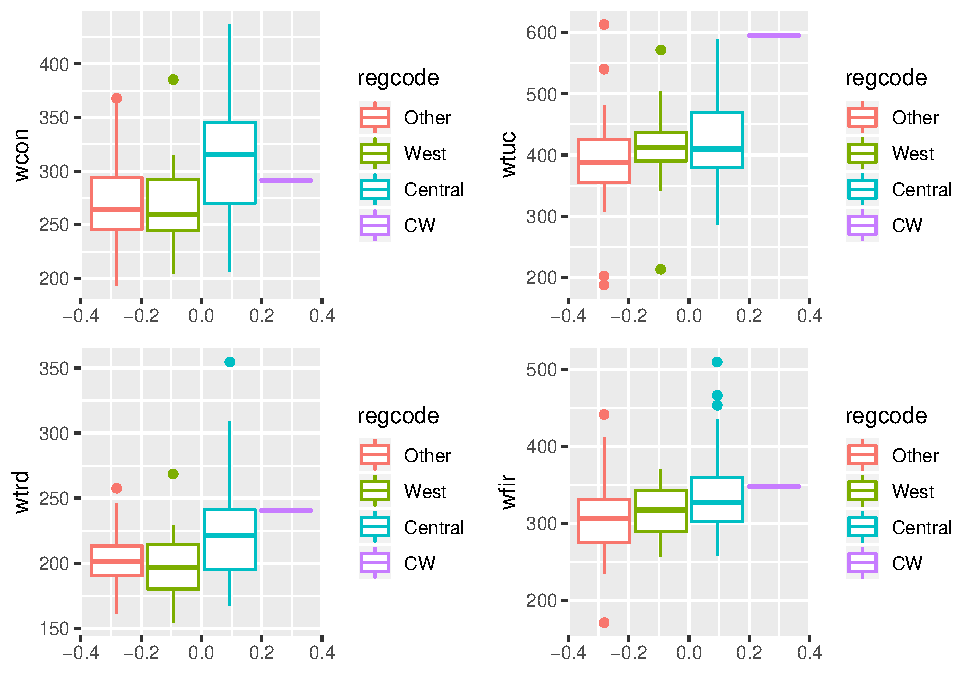
\includegraphics{Bagnard_Gaustad_Hartman_Leung_Lab_3_files/figure-latex/unnamed-chunk-15-1.pdf}

\begin{Shaded}
\begin{Highlighting}[]
\KeywordTok{grid.arrange}\NormalTok{(q3, q4, }\DataTypeTok{ncol=}\DecValTok{2}\NormalTok{)}
\end{Highlighting}
\end{Shaded}

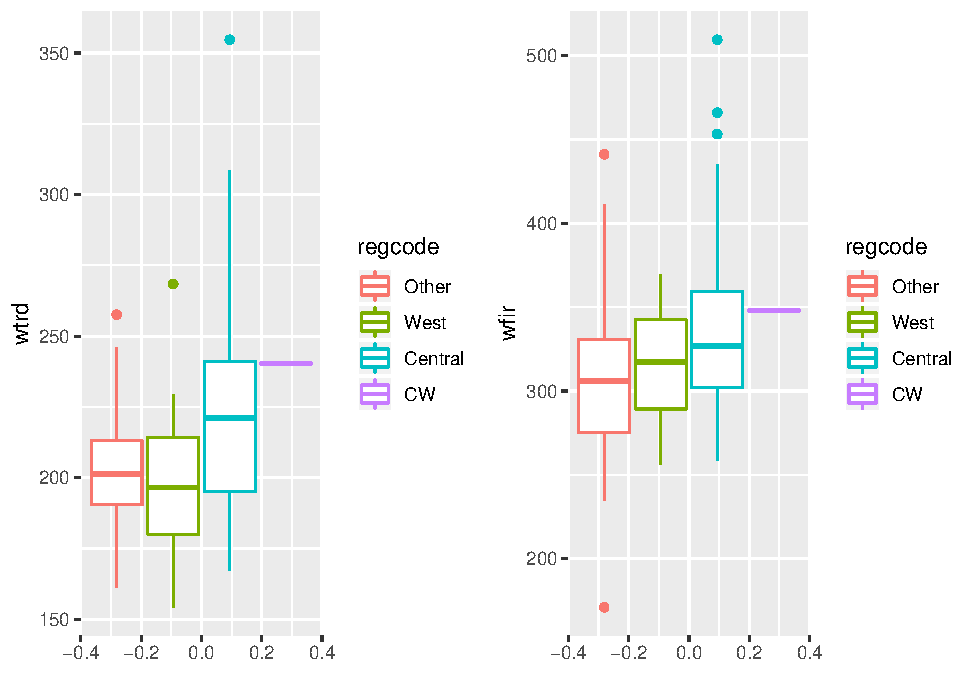
\includegraphics{Bagnard_Gaustad_Hartman_Leung_Lab_3_files/figure-latex/unnamed-chunk-15-2.pdf}

\begin{Shaded}
\begin{Highlighting}[]
\KeywordTok{grid.arrange}\NormalTok{(q5, q6, }\DataTypeTok{ncol=}\DecValTok{2}\NormalTok{)}
\end{Highlighting}
\end{Shaded}

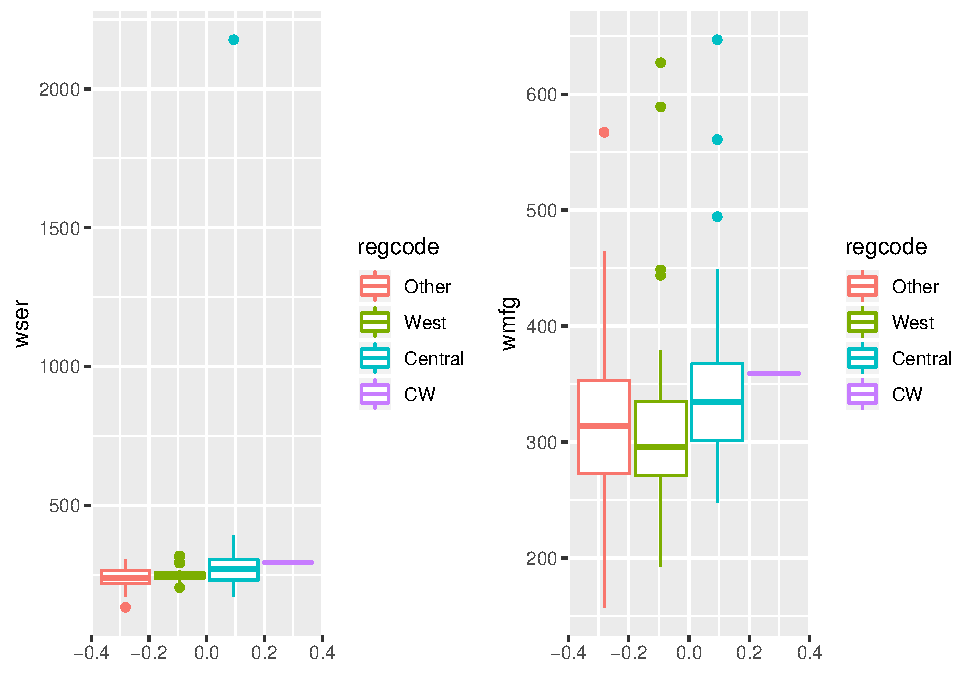
\includegraphics{Bagnard_Gaustad_Hartman_Leung_Lab_3_files/figure-latex/unnamed-chunk-15-3.pdf}

\begin{Shaded}
\begin{Highlighting}[]
\KeywordTok{grid.arrange}\NormalTok{(q7, q8, }\DataTypeTok{ncol=}\DecValTok{2}\NormalTok{)}
\end{Highlighting}
\end{Shaded}

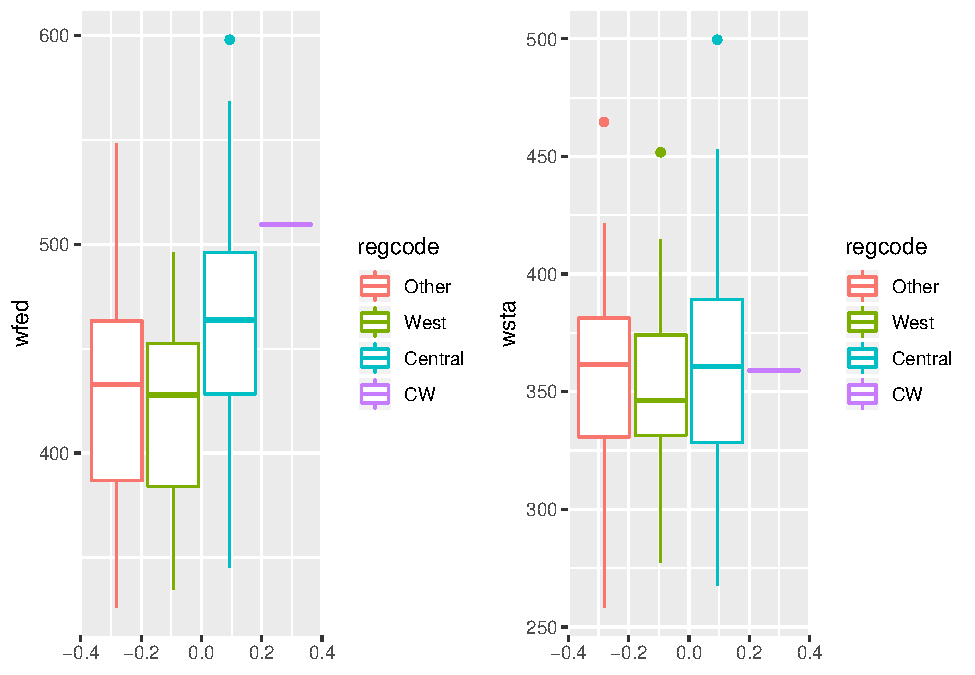
\includegraphics{Bagnard_Gaustad_Hartman_Leung_Lab_3_files/figure-latex/unnamed-chunk-15-4.pdf}

\begin{Shaded}
\begin{Highlighting}[]
\KeywordTok{grid.arrange}\NormalTok{(q9, q10, }\DataTypeTok{ncol=}\DecValTok{2}\NormalTok{)}
\end{Highlighting}
\end{Shaded}

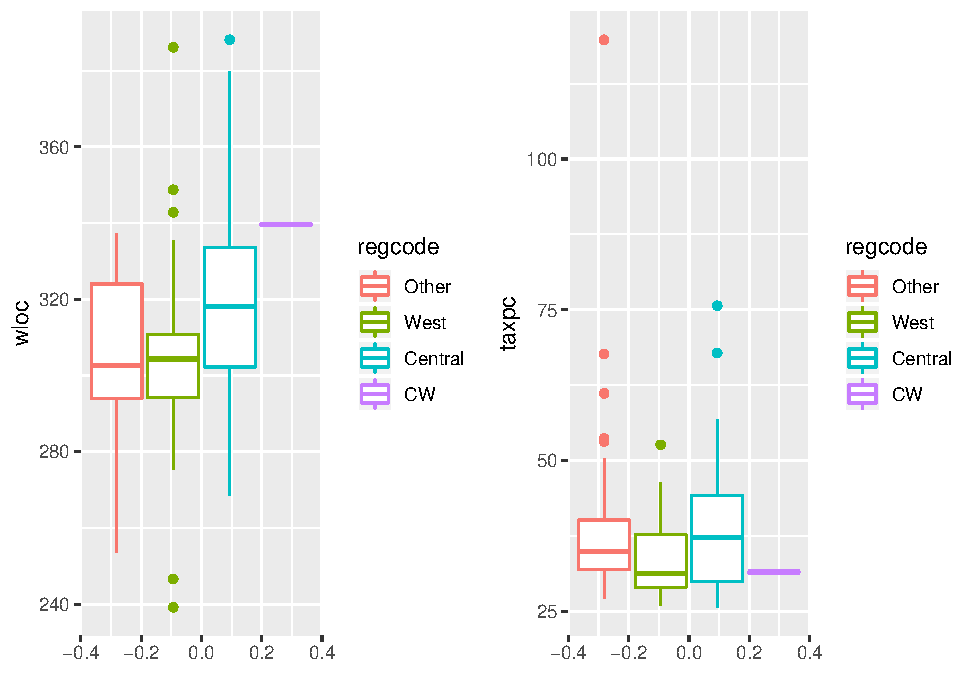
\includegraphics{Bagnard_Gaustad_Hartman_Leung_Lab_3_files/figure-latex/unnamed-chunk-15-5.pdf}

We observe a few data points of interest in the comparison above,
notably, wser appears to have an extreme data point.

Other variables show outliers as well, but not as extreme. We will
determine if any of these points have leverage or influence during model
specification.

For now, lets dig deeper into wser as we see it is an extreme outlier
from our visual inspection.

\begin{Shaded}
\begin{Highlighting}[]
\NormalTok{dfCrime }\OperatorTok
\KeywordTok{filter}\NormalTok{(wser }\OperatorTok{>}\StringTok{ }\DecValTok{2000}\NormalTok{) }\OperatorTok
\KeywordTok{select}\NormalTok{(county, wser)}
\end{Highlighting}
\end{Shaded}

\begin{verbatim}
  county     wser
1    185 2177.068
\end{verbatim}

This average service wage is much too high based on what we know about
the 1980s and every other wage recorded in comparison. A review of the
detailed population statistics describing mean wage per industry (table
231) confirms this.
\url{https://www2.census.gov/prod2/decennial/documents/1980/1980censusofpopu801352uns_bw.pdf}

Outliers affect our ability to estimate statistics, resulting in
overestimated or underestimated values. Outliers can be due to a number
of different factors such as response errors and data entry errors.
Outliers will introduce bias into our estimates and are addressed during
the analysis phase. The mechanism for treatment include three approaches

1 Trimming - \emph{remove} outliers from the dataset based on a maxima
or minima from the mean. 2 Winsorization - \emph{replace} extreme values
so they fall at the edge of the main distribution 3 Imputation -
\emph{recode} outliers by calculating the mean of the sample, or by
applying a regression model approach to predict the missing value

Trimming will remove the entire record. This is not an preferred
treatment as we will lose valuable information..

Winsorization is a symmetric process that will replace \emph{all} of the
smallest and largest data values in the sample. This is not a preferred
treatment as we will again lose valuable information, especially when we
only seek to replace values that are a result of a coding error.

Imputation recodes the data point using a predictive model derived from
the remainder of the sample data points. Multiple imputations are
performed to account for uncertainty, and each imputed data set is
analyzed for its distribution. Then, the mean, mode or median can be
chosen from this distribution as the replacement.

We favor the imputation method as we do not wish to apply Winsorization
to our data set wholistically, nor do we wish to remove the entire
observation and lose its contribution to other variables. Fortunately, a
number of packages are available in R that predict this value through
regression against the existing sample data. A commonly used imputation
library can be found in the Hmisc package which we will use for our
outlier treatment.

A full discussion of treatment methods can be found here:
\url{http://www.asasrms.org/Proceedings/y2004/files/Jsm2004-000559.pdf}

Finally, we should make note that none of these methods are ideal. We
would be better suited to discover the nature of the mistake and recode
it from real data. Since we do not have access to the underlying data
from which this sample set was derived we are not in the position to do
that. Thus we continue our analysis.

\begin{Shaded}
\begin{Highlighting}[]
\NormalTok{dfCrime}\OperatorTok{$}\NormalTok{wser[}\KeywordTok{which}\NormalTok{(dfCrime}\OperatorTok{$}\NormalTok{county}\OperatorTok{==}\DecValTok{185}\NormalTok{)]<-}\OtherTok{NA} \CommentTok{# set the value to NA so it will be imputed}
\end{Highlighting}
\end{Shaded}

\begin{Shaded}
\begin{Highlighting}[]
\NormalTok{impute_arg <-}\StringTok{ }\KeywordTok{aregImpute}\NormalTok{(}\OperatorTok{~}\StringTok{ }\NormalTok{crmrte }\OperatorTok{+}\StringTok{  }\NormalTok{urban }\OperatorTok{+}\StringTok{ }\NormalTok{central }\OperatorTok{+}\StringTok{ }\NormalTok{west }\OperatorTok{+}\StringTok{ }\NormalTok{other }\OperatorTok{+}
\StringTok{                         }\NormalTok{prbarr }\OperatorTok{+}\StringTok{ }\NormalTok{prbconv }\OperatorTok{+}\StringTok{ }\NormalTok{prbpris }\OperatorTok{+}\StringTok{ }\NormalTok{avgsen }\OperatorTok{+}\StringTok{ }\NormalTok{polpc }\OperatorTok{+}\StringTok{ }
\StringTok{                         }\NormalTok{density }\OperatorTok{+}\StringTok{ }\NormalTok{taxpc }\OperatorTok{+}\StringTok{ }\NormalTok{pctmin80 }\OperatorTok{+}\StringTok{ }\NormalTok{wcon }\OperatorTok{+}\StringTok{ }\NormalTok{wtuc }\OperatorTok{+}
\StringTok{                         }\NormalTok{wtrd }\OperatorTok{+}\StringTok{ }\NormalTok{wfir }\OperatorTok{+}\StringTok{ }\NormalTok{wser }\OperatorTok{+}\StringTok{ }\NormalTok{wmfg }\OperatorTok{+}\StringTok{ }\NormalTok{wfed }\OperatorTok{+}\StringTok{ }\NormalTok{wsta }\OperatorTok{+}\StringTok{ }\NormalTok{wloc }\OperatorTok{+}
\StringTok{                         }\NormalTok{mix }\OperatorTok{+}\StringTok{ }\NormalTok{pctymle, }\DataTypeTok{data =}\NormalTok{ dfCrime, }\DataTypeTok{match=}\StringTok{"weighted"}\NormalTok{,}
                         \DataTypeTok{nk=}\DecValTok{3}\NormalTok{, }\DataTypeTok{B=}\DecValTok{10}\NormalTok{, }\DataTypeTok{n.impute =} \DecValTok{100}\NormalTok{)}
\end{Highlighting}
\end{Shaded}

\begin{Shaded}
\begin{Highlighting}[]
\KeywordTok{paste}\NormalTok{(}\StringTok{"R-squares for Predicting Non-Missing Values for Each Variable"}\NormalTok{)}
\end{Highlighting}
\end{Shaded}

\begin{verbatim}
[1] "R-squares for Predicting Non-Missing Values for Each Variable"
\end{verbatim}

\begin{Shaded}
\begin{Highlighting}[]
\NormalTok{impute_arg}\OperatorTok{$}\NormalTok{rsq}
\end{Highlighting}
\end{Shaded}

\begin{verbatim}
     wser 
0.9407859 
\end{verbatim}

\begin{Shaded}
\begin{Highlighting}[]
\KeywordTok{paste}\NormalTok{(}\StringTok{"Distribution of Values for Each Imputation"}\NormalTok{)}
\end{Highlighting}
\end{Shaded}

\begin{verbatim}
[1] "Distribution of Values for Each Imputation"
\end{verbatim}

\begin{Shaded}
\begin{Highlighting}[]
\KeywordTok{table}\NormalTok{(impute_arg}\OperatorTok{$}\NormalTok{imputed}\OperatorTok{$}\NormalTok{wser)}
\end{Highlighting}
\end{Shaded}

\begin{verbatim}

133.0430603 172.4732666 172.6280975 182.0196228 192.3076935 196.1453247 
          9           4           2           3           2           2 
209.6972198 213.5821533 215.1933289 216.4588928 219.6342773 232.5915985 
          1           1           1           1           1           1 
239.2233429 246.0152435         250 253.0095825 256.4102478 256.7214355 
          1           2           1           1           1           1 
266.4674072 274.1774597 292.2253113 318.0335388 354.3007202 
          1          61           1           1           1 
\end{verbatim}

Note from the distribution above we see a mode appear from the multiple
imputation trials. One may argue that taking the mode is sufficient for
replacement. Taking a mode would be required if this were a categorical
value we were replacing. However, in this circumstance and to err on the
side of caution, we will reassign this value by taking the mean from the
trials.

\begin{Shaded}
\begin{Highlighting}[]
\NormalTok{dfCrime}\OperatorTok{$}\NormalTok{wser[}\KeywordTok{which}\NormalTok{(dfCrime}\OperatorTok{$}\NormalTok{county}\OperatorTok{==}\DecValTok{185}\NormalTok{)]<-}\KeywordTok{mean}\NormalTok{(impute_arg}\OperatorTok{$}\NormalTok{imputed}\OperatorTok{$}\NormalTok{wser)}
\KeywordTok{print}\NormalTok{(}\StringTok{"Newly Reassigned wser Value for County 185:"}\NormalTok{)}
\end{Highlighting}
\end{Shaded}

\begin{verbatim}
[1] "Newly Reassigned wser Value for County 185:"
\end{verbatim}

\begin{Shaded}
\begin{Highlighting}[]
\NormalTok{dfCrime}\OperatorTok{$}\NormalTok{wser[}\KeywordTok{which}\NormalTok{(dfCrime}\OperatorTok{$}\NormalTok{county}\OperatorTok{==}\DecValTok{185}\NormalTok{)]}
\end{Highlighting}
\end{Shaded}

\begin{verbatim}
[1] 245.6591
\end{verbatim}

Next, we will examine the criminal justice variables.

\begin{Shaded}
\begin{Highlighting}[]
\CommentTok{#Plot of the criminal justice and law enforcment related variables vs crmrte}
\NormalTok{q1<-}\KeywordTok{ggplot}\NormalTok{(}\DataTypeTok{data =}\NormalTok{ dfCrime, }\KeywordTok{aes}\NormalTok{(}\DataTypeTok{y =}\NormalTok{ prbarr, }\DataTypeTok{color =}\NormalTok{ regcode)) }\OperatorTok{+}\StringTok{ }
\StringTok{      }\KeywordTok{geom_boxplot}\NormalTok{()}
\NormalTok{q2<-}\KeywordTok{ggplot}\NormalTok{(}\DataTypeTok{data =}\NormalTok{ dfCrime, }\KeywordTok{aes}\NormalTok{(}\DataTypeTok{y =}\NormalTok{ prbconv, }\DataTypeTok{color =}\NormalTok{ regcode)) }\OperatorTok{+}\StringTok{ }
\StringTok{      }\KeywordTok{geom_boxplot}\NormalTok{()}
\NormalTok{q3<-}\KeywordTok{ggplot}\NormalTok{(}\DataTypeTok{data =}\NormalTok{ dfCrime, }\KeywordTok{aes}\NormalTok{(}\DataTypeTok{y =}\NormalTok{ prbpris, }\DataTypeTok{color =}\NormalTok{ regcode)) }\OperatorTok{+}\StringTok{ }
\StringTok{      }\KeywordTok{geom_boxplot}\NormalTok{()}
\NormalTok{q4<-}\KeywordTok{ggplot}\NormalTok{(}\DataTypeTok{data =}\NormalTok{ dfCrime, }\KeywordTok{aes}\NormalTok{(}\DataTypeTok{y =}\NormalTok{ avgsen, }\DataTypeTok{color =}\NormalTok{ regcode)) }\OperatorTok{+}\StringTok{ }
\StringTok{      }\KeywordTok{geom_boxplot}\NormalTok{()}
\NormalTok{q5<-}\KeywordTok{ggplot}\NormalTok{(}\DataTypeTok{data =}\NormalTok{ dfCrime, }\KeywordTok{aes}\NormalTok{(}\DataTypeTok{y =}\NormalTok{ polpc, }\DataTypeTok{color =}\NormalTok{ regcode)) }\OperatorTok{+}\StringTok{ }
\StringTok{      }\KeywordTok{geom_boxplot}\NormalTok{()}
\NormalTok{q6<-}\KeywordTok{ggplot}\NormalTok{(}\DataTypeTok{data =}\NormalTok{ dfCrime, }\KeywordTok{aes}\NormalTok{(}\DataTypeTok{y =}\NormalTok{ mix, }\DataTypeTok{color =}\NormalTok{ regcode)) }\OperatorTok{+}\StringTok{ }
\StringTok{      }\KeywordTok{geom_boxplot}\NormalTok{()}

\KeywordTok{grid.arrange}\NormalTok{(q1, q2, }\DataTypeTok{ncol=}\DecValTok{2}\NormalTok{)}
\end{Highlighting}
\end{Shaded}

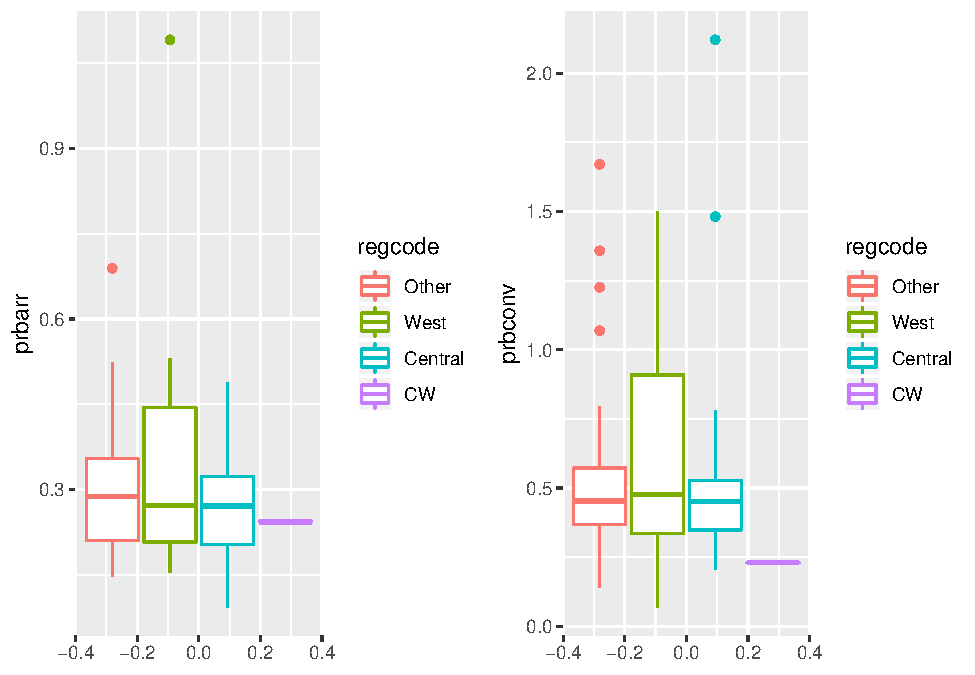
\includegraphics{Bagnard_Gaustad_Hartman_Leung_Lab_3_files/figure-latex/unnamed-chunk-22-1.pdf}

\begin{Shaded}
\begin{Highlighting}[]
\KeywordTok{grid.arrange}\NormalTok{(q3, q4, }\DataTypeTok{ncol=}\DecValTok{2}\NormalTok{)}
\end{Highlighting}
\end{Shaded}

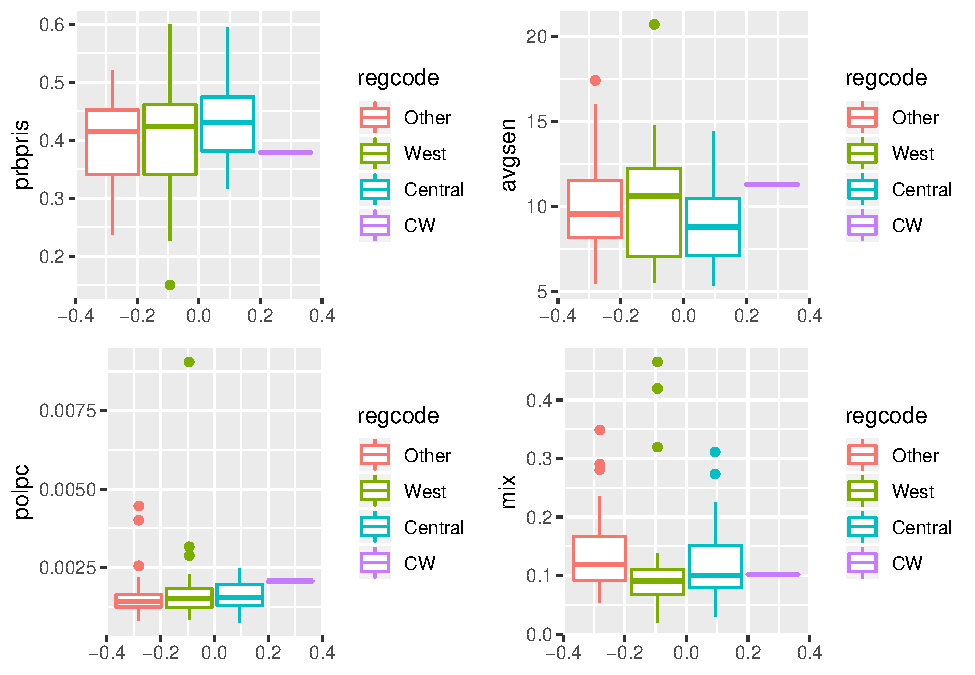
\includegraphics{Bagnard_Gaustad_Hartman_Leung_Lab_3_files/figure-latex/unnamed-chunk-22-2.pdf}

\begin{Shaded}
\begin{Highlighting}[]
\KeywordTok{grid.arrange}\NormalTok{(q5, q6, }\DataTypeTok{ncol=}\DecValTok{2}\NormalTok{)}
\end{Highlighting}
\end{Shaded}

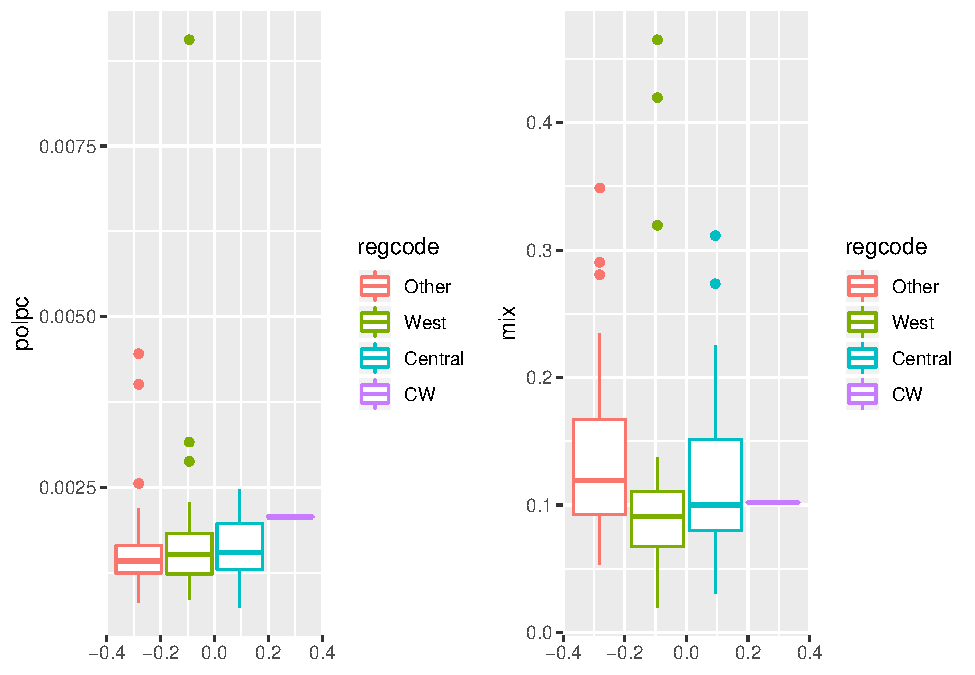
\includegraphics{Bagnard_Gaustad_Hartman_Leung_Lab_3_files/figure-latex/unnamed-chunk-22-3.pdf}

The criminal justice and law enforcement variables show evidence of
outliers, notably, pbarr and polpc appear to have extreme data points.

Upon further inspection, the extreme outlier value for polpc is .009.
Based on records describing the US population on police officers per
capita, the highest police per capita on record for United States
counties is .007 in Atlantic City, NJ.
\url{https://www.governing.com/gov-data/safety-justice/police-officers-per-capita-rates-employment-for-city-departments.html}
This datapoint is an error and we will impute it's replacement.

\begin{Shaded}
\begin{Highlighting}[]
\NormalTok{dfCrime}\OperatorTok{$}\NormalTok{polpc[}\KeywordTok{which}\NormalTok{(dfCrime}\OperatorTok{$}\NormalTok{county}\OperatorTok{==}\DecValTok{115}\NormalTok{)]<-}\OtherTok{NA} \CommentTok{# set the value to NA so it will be imputed}
\end{Highlighting}
\end{Shaded}

\begin{Shaded}
\begin{Highlighting}[]
\NormalTok{impute_arg <-}\StringTok{ }\KeywordTok{aregImpute}\NormalTok{(}\OperatorTok{~}\StringTok{ }\NormalTok{crmrte }\OperatorTok{+}\StringTok{  }\NormalTok{urban }\OperatorTok{+}\StringTok{ }\NormalTok{central }\OperatorTok{+}\StringTok{ }\NormalTok{west }\OperatorTok{+}\StringTok{ }\NormalTok{other }\OperatorTok{+}
\StringTok{                         }\NormalTok{prbarr }\OperatorTok{+}\StringTok{ }\NormalTok{prbconv }\OperatorTok{+}\StringTok{ }\NormalTok{prbpris }\OperatorTok{+}\StringTok{ }\NormalTok{avgsen }\OperatorTok{+}\StringTok{ }\NormalTok{polpc }\OperatorTok{+}\StringTok{ }
\StringTok{                         }\NormalTok{density }\OperatorTok{+}\StringTok{ }\NormalTok{taxpc }\OperatorTok{+}\StringTok{ }\NormalTok{pctmin80 }\OperatorTok{+}\StringTok{ }\NormalTok{wcon }\OperatorTok{+}\StringTok{ }\NormalTok{wtuc }\OperatorTok{+}
\StringTok{                         }\NormalTok{wtrd }\OperatorTok{+}\StringTok{ }\NormalTok{wfir }\OperatorTok{+}\StringTok{ }\NormalTok{wser }\OperatorTok{+}\StringTok{ }\NormalTok{wmfg }\OperatorTok{+}\StringTok{ }\NormalTok{wfed }\OperatorTok{+}\StringTok{ }\NormalTok{wsta }\OperatorTok{+}\StringTok{ }\NormalTok{wloc }\OperatorTok{+}
\StringTok{                         }\NormalTok{mix }\OperatorTok{+}\StringTok{ }\NormalTok{pctymle, }\DataTypeTok{data =}\NormalTok{ dfCrime, }\DataTypeTok{match=}\StringTok{"weighted"}\NormalTok{,}
                         \DataTypeTok{nk=}\DecValTok{3}\NormalTok{, }\DataTypeTok{B=}\DecValTok{10}\NormalTok{, }\DataTypeTok{n.impute =} \DecValTok{100}\NormalTok{)}
\end{Highlighting}
\end{Shaded}

\begin{Shaded}
\begin{Highlighting}[]
\KeywordTok{paste}\NormalTok{(}\StringTok{"R-squares for Predicting Non-Missing Values for Each Variable"}\NormalTok{)}
\end{Highlighting}
\end{Shaded}

\begin{verbatim}
[1] "R-squares for Predicting Non-Missing Values for Each Variable"
\end{verbatim}

\begin{Shaded}
\begin{Highlighting}[]
\NormalTok{impute_arg}\OperatorTok{$}\NormalTok{rsq}
\end{Highlighting}
\end{Shaded}

\begin{verbatim}
    polpc 
0.8595967 
\end{verbatim}

\begin{Shaded}
\begin{Highlighting}[]
\KeywordTok{paste}\NormalTok{(}\StringTok{"Predicted values"}\NormalTok{)}
\end{Highlighting}
\end{Shaded}

\begin{verbatim}
[1] "Predicted values"
\end{verbatim}

\begin{Shaded}
\begin{Highlighting}[]
\KeywordTok{mean}\NormalTok{(impute_arg}\OperatorTok{$}\NormalTok{imputed}\OperatorTok{$}\NormalTok{polpc)}
\end{Highlighting}
\end{Shaded}

\begin{verbatim}
[1] 0.002624843
\end{verbatim}

We will reassign this value using the mean from the trials.

\begin{Shaded}
\begin{Highlighting}[]
\NormalTok{dfCrime}\OperatorTok{$}\NormalTok{polpc[}\KeywordTok{which}\NormalTok{(dfCrime}\OperatorTok{$}\NormalTok{county}\OperatorTok{==}\DecValTok{115}\NormalTok{)]<-}\KeywordTok{mean}\NormalTok{(impute_arg}\OperatorTok{$}\NormalTok{imputed}\OperatorTok{$}\NormalTok{polpc)}
\end{Highlighting}
\end{Shaded}

Our analysis into the demographic data is next.

\begin{Shaded}
\begin{Highlighting}[]
\CommentTok{#plot of demographic information for counties Outside and Inside the metro areas}
\CommentTok{# population density, percent minority, percent young male}

\KeywordTok{ggplot}\NormalTok{(}\DataTypeTok{data =}\NormalTok{ dfCrime, }\KeywordTok{aes}\NormalTok{(}\DataTypeTok{y =}\NormalTok{ density, }\DataTypeTok{color =}\NormalTok{ regcode)) }\OperatorTok{+}\StringTok{ }
\StringTok{      }\KeywordTok{geom_boxplot}\NormalTok{() }\OperatorTok{+}\StringTok{ }\KeywordTok{facet_wrap}\NormalTok{(}\OperatorTok{~}\StringTok{ }\NormalTok{metro)}
\end{Highlighting}
\end{Shaded}

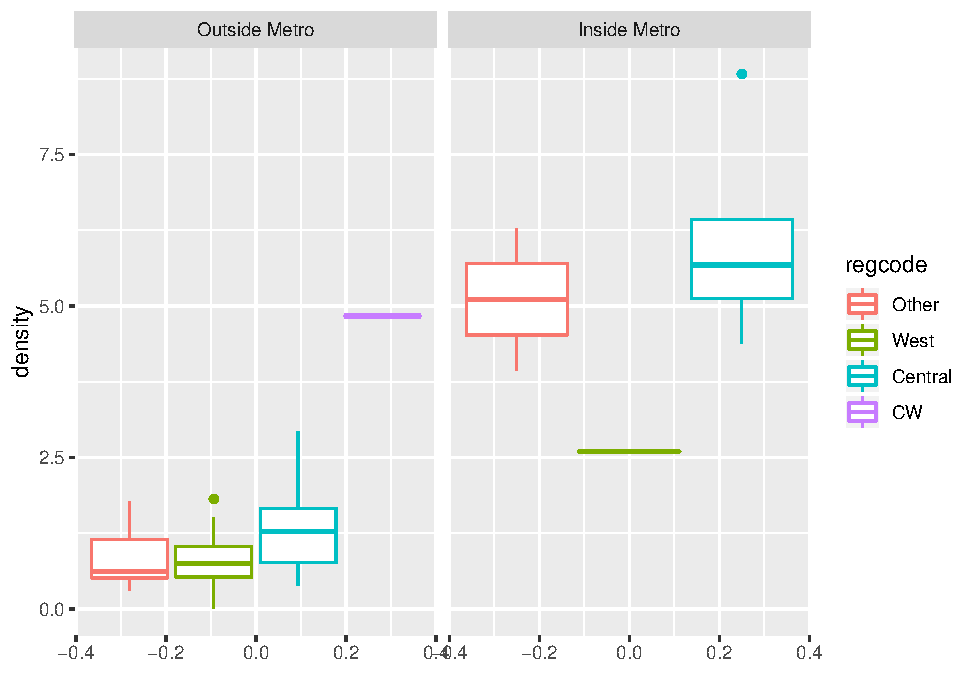
\includegraphics{Bagnard_Gaustad_Hartman_Leung_Lab_3_files/figure-latex/unnamed-chunk-27-1.pdf}

\begin{Shaded}
\begin{Highlighting}[]
\KeywordTok{ggplot}\NormalTok{(}\DataTypeTok{data =}\NormalTok{ dfCrime, }\KeywordTok{aes}\NormalTok{(}\DataTypeTok{y =}\NormalTok{ pctmin80, }\DataTypeTok{color =}\NormalTok{ regcode)) }\OperatorTok{+}\StringTok{ }
\StringTok{      }\KeywordTok{geom_boxplot}\NormalTok{() }\OperatorTok{+}\StringTok{ }\KeywordTok{facet_wrap}\NormalTok{(}\OperatorTok{~}\StringTok{ }\NormalTok{metro)}
\end{Highlighting}
\end{Shaded}

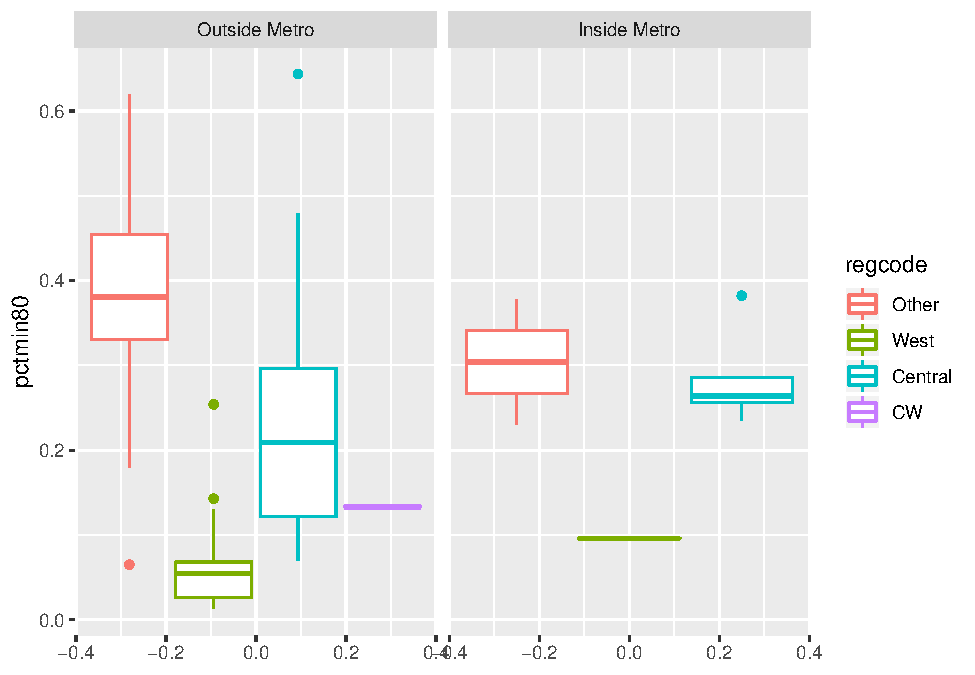
\includegraphics{Bagnard_Gaustad_Hartman_Leung_Lab_3_files/figure-latex/unnamed-chunk-27-2.pdf}

\begin{Shaded}
\begin{Highlighting}[]
\KeywordTok{ggplot}\NormalTok{(}\DataTypeTok{data =}\NormalTok{ dfCrime, }\KeywordTok{aes}\NormalTok{(}\DataTypeTok{y =}\NormalTok{ pctymle, }\DataTypeTok{color =}\NormalTok{ regcode)) }\OperatorTok{+}\StringTok{ }
\StringTok{      }\KeywordTok{geom_boxplot}\NormalTok{() }\OperatorTok{+}\StringTok{ }\KeywordTok{facet_wrap}\NormalTok{(}\OperatorTok{~}\StringTok{ }\NormalTok{metro)}
\end{Highlighting}
\end{Shaded}

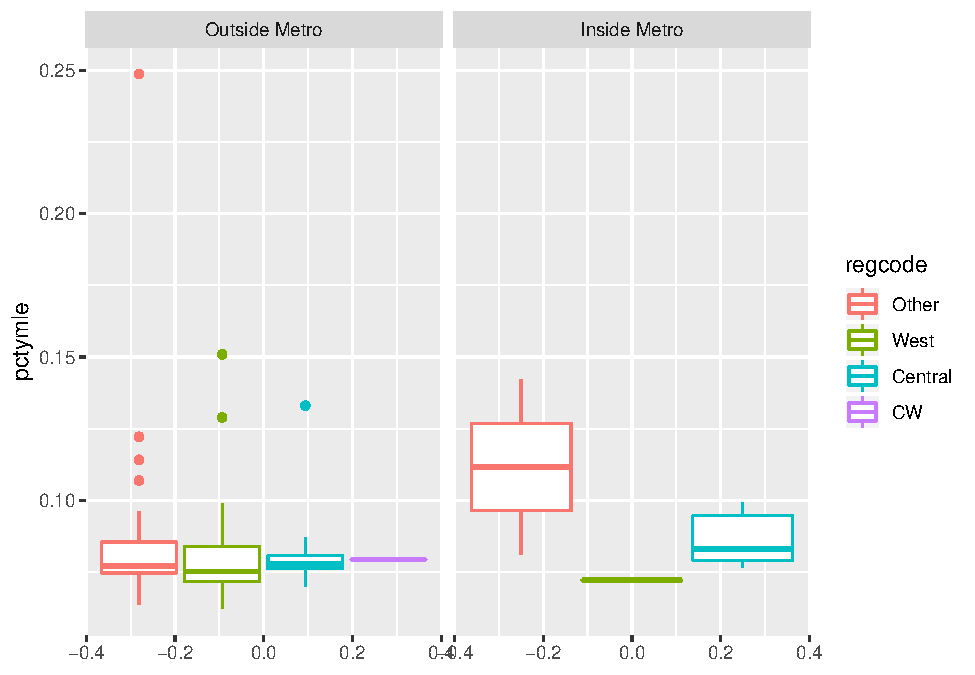
\includegraphics{Bagnard_Gaustad_Hartman_Leung_Lab_3_files/figure-latex/unnamed-chunk-27-3.pdf}

Notably more outliers are observed in demographic information. Here,
pctymle in one county outside of a metro area is nearly 25\%. That seems
quite high in normal statistical measures of the population. However,
this can be explained as being county with a large college town
population. Specifically, Appalachian State University in Watauga County
(\url{https://en.wikipedia.org/wiki/Watauga_County,_North_Carolina}),
where the presense of the university notably affects the overall age
distribution and median age. This is further confirmed in county
estimate records here:
\url{https://www.osbm.nc.gov/demog/county-estimates}.

Finally, we can see our CW encoded county and where it appears in
population density. It is clearly not an outside metro county. In
addition to being improperly coded for both western and central regions
it appears to be miscoded for its metro characteristics as well.

We will address the metro variable, and examine whether the region
should be `west', `central' or `other' instead of both central and west

\begin{Shaded}
\begin{Highlighting}[]
\NormalTok{dfCrime }\OperatorTok
\CommentTok{#filter(west ==1 & central ==1) %>%}
\KeywordTok{filter}\NormalTok{(density }\OperatorTok{>}\StringTok{ }\FloatTok{2.5}\NormalTok{) }\OperatorTok
\KeywordTok{select}\NormalTok{(county, west, central, other, urban, region, regcode, metro)}
\end{Highlighting}
\end{Shaded}

\begin{verbatim}
   county west central other urban region regcode         metro
1      21    1       0     0     1      1    West  Inside Metro
2      25    0       1     0     0      2 Central Outside Metro
3      35    0       1     0     0      2 Central Outside Metro
4      51    0       0     1     1      0   Other  Inside Metro
5      63    0       1     0     1      2 Central  Inside Metro
6      67    0       1     0     1      2 Central  Inside Metro
7      71    1       1     0     0      3      CW Outside Metro
8      81    0       1     0     1      2 Central  Inside Metro
9     119    0       1     0     1      2 Central  Inside Metro
10    129    0       0     1     1      0   Other  Inside Metro
11    183    0       1     0     1      2 Central  Inside Metro
\end{verbatim}

\begin{Shaded}
\begin{Highlighting}[]
\NormalTok{dfCrime}\OperatorTok{$}\NormalTok{west[}\KeywordTok{which}\NormalTok{(dfCrime}\OperatorTok{$}\NormalTok{county}\OperatorTok{==}\DecValTok{71}\NormalTok{)]<-}\OtherTok{NA}
\NormalTok{dfCrime}\OperatorTok{$}\NormalTok{central[}\KeywordTok{which}\NormalTok{(dfCrime}\OperatorTok{$}\NormalTok{county}\OperatorTok{==}\DecValTok{71}\NormalTok{)]<-}\OtherTok{NA}
\NormalTok{dfCrime}\OperatorTok{$}\NormalTok{other[}\KeywordTok{which}\NormalTok{(dfCrime}\OperatorTok{$}\NormalTok{county}\OperatorTok{==}\DecValTok{71}\NormalTok{)]<-}\OtherTok{NA}
\NormalTok{dfCrime}\OperatorTok{$}\NormalTok{urban[}\KeywordTok{which}\NormalTok{(dfCrime}\OperatorTok{$}\NormalTok{county}\OperatorTok{==}\DecValTok{71}\NormalTok{)]<-}\OtherTok{NA}
\end{Highlighting}
\end{Shaded}

\begin{Shaded}
\begin{Highlighting}[]
\NormalTok{impute_arg <-}\StringTok{ }\KeywordTok{aregImpute}\NormalTok{(}\OperatorTok{~}\StringTok{ }\NormalTok{crmrte }\OperatorTok{+}\StringTok{  }\NormalTok{urban }\OperatorTok{+}\StringTok{ }\NormalTok{central }\OperatorTok{+}\StringTok{ }\NormalTok{west }\OperatorTok{+}
\StringTok{                         }\NormalTok{prbarr }\OperatorTok{+}\StringTok{ }\NormalTok{prbconv }\OperatorTok{+}\StringTok{ }\NormalTok{prbpris }\OperatorTok{+}\StringTok{ }\NormalTok{avgsen }\OperatorTok{+}\StringTok{ }\NormalTok{polpc }\OperatorTok{+}\StringTok{ }
\StringTok{                         }\NormalTok{density }\OperatorTok{+}\StringTok{ }\NormalTok{taxpc }\OperatorTok{+}\StringTok{ }\NormalTok{pctmin80 }\OperatorTok{+}\StringTok{ }\NormalTok{wcon }\OperatorTok{+}\StringTok{ }\NormalTok{wtuc }\OperatorTok{+}
\StringTok{                         }\NormalTok{wtrd }\OperatorTok{+}\StringTok{ }\NormalTok{wfir }\OperatorTok{+}\StringTok{ }\NormalTok{wser }\OperatorTok{+}\StringTok{ }\NormalTok{wmfg }\OperatorTok{+}\StringTok{ }\NormalTok{wfed }\OperatorTok{+}\StringTok{ }\NormalTok{wsta }\OperatorTok{+}\StringTok{ }\NormalTok{wloc }\OperatorTok{+}
\StringTok{                         }\NormalTok{mix }\OperatorTok{+}\StringTok{ }\NormalTok{pctymle, }\DataTypeTok{data =}\NormalTok{ dfCrime, }\DataTypeTok{match=}\StringTok{"weighted"}\NormalTok{,}
                         \DataTypeTok{nk=}\DecValTok{3}\NormalTok{, }\DataTypeTok{B=}\DecValTok{10}\NormalTok{, }\DataTypeTok{n.impute =} \DecValTok{100}\NormalTok{)}
\end{Highlighting}
\end{Shaded}

\begin{Shaded}
\begin{Highlighting}[]
\KeywordTok{paste}\NormalTok{(}\StringTok{"R-squares for Predicting Non-Missing Values for Each Variable"}\NormalTok{)}
\end{Highlighting}
\end{Shaded}

\begin{verbatim}
[1] "R-squares for Predicting Non-Missing Values for Each Variable"
\end{verbatim}

\begin{Shaded}
\begin{Highlighting}[]
\NormalTok{impute_arg}\OperatorTok{$}\NormalTok{rsq}
\end{Highlighting}
\end{Shaded}

\begin{verbatim}
    urban   central      west 
0.9605375 0.8871089 0.9825171 
\end{verbatim}

\begin{Shaded}
\begin{Highlighting}[]
\KeywordTok{paste}\NormalTok{(}\StringTok{"Predicted values"}\NormalTok{)}
\end{Highlighting}
\end{Shaded}

\begin{verbatim}
[1] "Predicted values"
\end{verbatim}

\begin{Shaded}
\begin{Highlighting}[]
\KeywordTok{Mode}\NormalTok{(impute_arg}\OperatorTok{$}\NormalTok{imputed}\OperatorTok{$}\NormalTok{urban)}
\end{Highlighting}
\end{Shaded}

\begin{verbatim}
[1] 1
\end{verbatim}

\begin{Shaded}
\begin{Highlighting}[]
\KeywordTok{Mode}\NormalTok{(impute_arg}\OperatorTok{$}\NormalTok{imputed}\OperatorTok{$}\NormalTok{central)}
\end{Highlighting}
\end{Shaded}

\begin{verbatim}
[1] 1
\end{verbatim}

\begin{Shaded}
\begin{Highlighting}[]
\KeywordTok{Mode}\NormalTok{(impute_arg}\OperatorTok{$}\NormalTok{imputed}\OperatorTok{$}\NormalTok{west)}
\end{Highlighting}
\end{Shaded}

\begin{verbatim}
[1] 0
\end{verbatim}

The results confirm the county is urban. It is also highly probable that
county 71 is not west and most likely associated with central. After
correcting our data for urban and west, let's compare `central' with
`other' to be certain we have the right region.

\begin{Shaded}
\begin{Highlighting}[]
\NormalTok{dfCrime}\OperatorTok{$}\NormalTok{urban[}\KeywordTok{which}\NormalTok{(dfCrime}\OperatorTok{$}\NormalTok{county}\OperatorTok{==}\DecValTok{71}\NormalTok{)]<-}\KeywordTok{Mode}\NormalTok{(impute_arg}\OperatorTok{$}\NormalTok{imputed}\OperatorTok{$}\NormalTok{urban)}
\NormalTok{dfCrime}\OperatorTok{$}\NormalTok{nonurban[}\KeywordTok{which}\NormalTok{(dfCrime}\OperatorTok{$}\NormalTok{county}\OperatorTok{==}\DecValTok{71}\NormalTok{)]<-}\DecValTok{1}\OperatorTok{-}\KeywordTok{Mode}\NormalTok{(impute_arg}\OperatorTok{$}\NormalTok{imputed}\OperatorTok{$}\NormalTok{urban)}
\NormalTok{dfCrime}\OperatorTok{$}\NormalTok{west[}\KeywordTok{which}\NormalTok{(dfCrime}\OperatorTok{$}\NormalTok{county}\OperatorTok{==}\DecValTok{71}\NormalTok{)]<-}\KeywordTok{Mode}\NormalTok{(impute_arg}\OperatorTok{$}\NormalTok{imputed}\OperatorTok{$}\NormalTok{west)}
\NormalTok{dfCrime}\OperatorTok{$}\NormalTok{metro[}\KeywordTok{which}\NormalTok{(dfCrime}\OperatorTok{$}\NormalTok{county}\OperatorTok{==}\DecValTok{71}\NormalTok{)]<-}\StringTok{'Inside Metro'}
\end{Highlighting}
\end{Shaded}

\begin{Shaded}
\begin{Highlighting}[]
\NormalTok{impute_arg <-}\StringTok{ }\KeywordTok{aregImpute}\NormalTok{(}\OperatorTok{~}\StringTok{ }\NormalTok{crmrte }\OperatorTok{+}\StringTok{ }\NormalTok{central }\OperatorTok{+}\StringTok{ }\NormalTok{other }\OperatorTok{+}
\StringTok{                         }\NormalTok{prbarr }\OperatorTok{+}\StringTok{ }\NormalTok{prbconv }\OperatorTok{+}\StringTok{ }\NormalTok{prbpris }\OperatorTok{+}\StringTok{ }\NormalTok{avgsen }\OperatorTok{+}\StringTok{ }\NormalTok{polpc }\OperatorTok{+}\StringTok{ }
\StringTok{                         }\NormalTok{density }\OperatorTok{+}\StringTok{ }\NormalTok{taxpc }\OperatorTok{+}\StringTok{ }\NormalTok{pctmin80 }\OperatorTok{+}\StringTok{ }\NormalTok{wcon }\OperatorTok{+}\StringTok{ }\NormalTok{wtuc }\OperatorTok{+}
\StringTok{                         }\NormalTok{wtrd }\OperatorTok{+}\StringTok{ }\NormalTok{wfir }\OperatorTok{+}\StringTok{ }\NormalTok{wser }\OperatorTok{+}\StringTok{ }\NormalTok{wmfg }\OperatorTok{+}\StringTok{ }\NormalTok{wfed }\OperatorTok{+}\StringTok{ }\NormalTok{wsta }\OperatorTok{+}\StringTok{ }\NormalTok{wloc }\OperatorTok{+}
\StringTok{                         }\NormalTok{mix }\OperatorTok{+}\StringTok{ }\NormalTok{pctymle, }\DataTypeTok{data =}\NormalTok{ dfCrime, }\DataTypeTok{match=}\StringTok{"weighted"}\NormalTok{,}
                         \DataTypeTok{nk=}\DecValTok{3}\NormalTok{, }\DataTypeTok{B=}\DecValTok{10}\NormalTok{, }\DataTypeTok{n.impute =} \DecValTok{100}\NormalTok{)}
\end{Highlighting}
\end{Shaded}

\begin{Shaded}
\begin{Highlighting}[]
\KeywordTok{paste}\NormalTok{(}\StringTok{"R-squares for Predicting Non-Missing Values for Each Variable"}\NormalTok{)}
\end{Highlighting}
\end{Shaded}

\begin{verbatim}
[1] "R-squares for Predicting Non-Missing Values for Each Variable"
\end{verbatim}

\begin{Shaded}
\begin{Highlighting}[]
\NormalTok{impute_arg}\OperatorTok{$}\NormalTok{rsq}
\end{Highlighting}
\end{Shaded}

\begin{verbatim}
  central     other 
0.9131930 0.9235304 
\end{verbatim}

\begin{Shaded}
\begin{Highlighting}[]
\KeywordTok{paste}\NormalTok{(}\StringTok{"Predicted values"}\NormalTok{)}
\end{Highlighting}
\end{Shaded}

\begin{verbatim}
[1] "Predicted values"
\end{verbatim}

\begin{Shaded}
\begin{Highlighting}[]
\KeywordTok{Mode}\NormalTok{(impute_arg}\OperatorTok{$}\NormalTok{imputed}\OperatorTok{$}\NormalTok{other)}
\end{Highlighting}
\end{Shaded}

\begin{verbatim}
[1] 0
\end{verbatim}

We show with high degree of certainty that the county is not `other'.
The case for central is high. Since the county is not western and not
other it is central by process of elimination, and the Hmisc algorithm
bolsters that suggestion. We'll assign our new values.

\begin{Shaded}
\begin{Highlighting}[]
\NormalTok{dfCrime}\OperatorTok{$}\NormalTok{other[}\KeywordTok{which}\NormalTok{(dfCrime}\OperatorTok{$}\NormalTok{county}\OperatorTok{==}\DecValTok{71}\NormalTok{)]<-}\KeywordTok{Mode}\NormalTok{(impute_arg}\OperatorTok{$}\NormalTok{imputed}\OperatorTok{$}\NormalTok{other)}
\NormalTok{dfCrime}\OperatorTok{$}\NormalTok{central[}\KeywordTok{which}\NormalTok{(dfCrime}\OperatorTok{$}\NormalTok{county}\OperatorTok{==}\DecValTok{71}\NormalTok{)]<-}\DecValTok{1}\OperatorTok{-}\KeywordTok{Mode}\NormalTok{(impute_arg}\OperatorTok{$}\NormalTok{imputed}\OperatorTok{$}\NormalTok{other)}
\NormalTok{dfCrime}\OperatorTok{$}\NormalTok{region[}\KeywordTok{which}\NormalTok{(dfCrime}\OperatorTok{$}\NormalTok{county}\OperatorTok{==}\DecValTok{71}\NormalTok{)]<-}\StringTok{ }\DecValTok{2} \CommentTok{#Central}
\NormalTok{dfCrime}\OperatorTok{$}\NormalTok{regcode[}\KeywordTok{which}\NormalTok{(dfCrime}\OperatorTok{$}\NormalTok{county}\OperatorTok{==}\DecValTok{71}\NormalTok{)]<-}\StringTok{ 'Central'}
\end{Highlighting}
\end{Shaded}

We also wish to examine the density variable in more detail by looking
at its distribution.

\begin{Shaded}
\begin{Highlighting}[]
\KeywordTok{options}\NormalTok{(}\DataTypeTok{repr.plot.width=}\DecValTok{8}\NormalTok{, }\DataTypeTok{repr.plot.height=}\DecValTok{4}\NormalTok{)}
\KeywordTok{ggplot}\NormalTok{(}\DataTypeTok{data =}\NormalTok{ dfCrime, }\KeywordTok{aes}\NormalTok{(}\DataTypeTok{x =}\NormalTok{ density)) }\OperatorTok{+}\StringTok{ }
\StringTok{      }\KeywordTok{geom_histogram}\NormalTok{(}\DataTypeTok{bins=}\DecValTok{90}\NormalTok{)}
\end{Highlighting}
\end{Shaded}

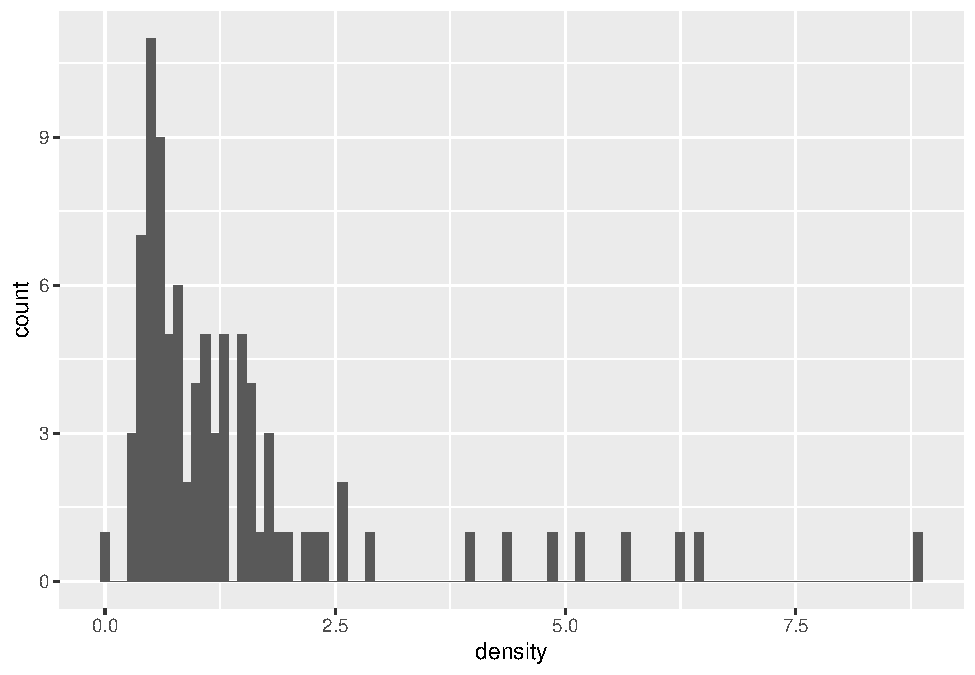
\includegraphics{Bagnard_Gaustad_Hartman_Leung_Lab_3_files/figure-latex/unnamed-chunk-37-1.pdf}

We note that one of the counties has an extremely low density. Near
zero.

\begin{Shaded}
\begin{Highlighting}[]
\NormalTok{dfCrime }\OperatorTok
\KeywordTok{filter}\NormalTok{(density }\OperatorTok{<}\StringTok{ }\FloatTok{0.01}\NormalTok{)}
\end{Highlighting}
\end{Shaded}

\begin{verbatim}
  county year    crmrte   prbarr  prbconv prbpris avgsen      polpc
1    173   87 0.0139937 0.530435 0.327869    0.15   6.64 0.00316379
      density    taxpc west central urban pctmin80    wcon     wtuc
1 2.03422e-05 37.72702    1       0     0 0.253914 231.696 213.6752
      wtrd    wfir     wser   wmfg   wfed   wsta   wloc       mix
1 175.1604 267.094 204.3792 193.01 334.44 414.68 304.32 0.4197531
     pctymle region regcode other nonurban         metro
1 0.07462687      1    West     0        1 Outside Metro
\end{verbatim}

In review of the North Carolina county density data from 1985, the
smallest population density in any county in North Carolina is 0.0952.
\url{http://ncosbm.s3.amazonaws.com/s3fs-public/demog/dens7095.xls}

This makes the density of 0.0000203422 (ie. average of
\textasciitilde{}2.0 people per 10,000 square miles) for county 173
statistically impossible. It is miscoded.

\begin{Shaded}
\begin{Highlighting}[]
\NormalTok{dfCrime}\OperatorTok{$}\NormalTok{density[}\KeywordTok{which}\NormalTok{(dfCrime}\OperatorTok{$}\NormalTok{county}\OperatorTok{==}\DecValTok{173}\NormalTok{)]<-}\StringTok{ }\OtherTok{NA}
\end{Highlighting}
\end{Shaded}

\begin{Shaded}
\begin{Highlighting}[]
\CommentTok{#dfSubset <-  we will use the non-urban western counties}
\NormalTok{impute_arg <-}\StringTok{ }\KeywordTok{aregImpute}\NormalTok{(}\OperatorTok{~}\StringTok{ }\NormalTok{crmrte }\OperatorTok{+}
\StringTok{                         }\NormalTok{prbarr }\OperatorTok{+}\StringTok{ }\NormalTok{prbconv }\OperatorTok{+}\StringTok{ }\NormalTok{prbpris }\OperatorTok{+}\StringTok{ }\NormalTok{avgsen }\OperatorTok{+}\StringTok{ }\NormalTok{polpc }\OperatorTok{+}\StringTok{ }
\StringTok{                         }\NormalTok{density }\OperatorTok{+}\StringTok{ }\NormalTok{taxpc }\OperatorTok{+}\StringTok{ }\NormalTok{pctmin80 }\OperatorTok{+}\StringTok{ }\NormalTok{wcon }\OperatorTok{+}\StringTok{ }\NormalTok{wtuc }\OperatorTok{+}
\StringTok{                         }\NormalTok{wtrd }\OperatorTok{+}\StringTok{ }\NormalTok{wfir }\OperatorTok{+}\StringTok{ }\NormalTok{wser }\OperatorTok{+}\StringTok{ }\NormalTok{wmfg }\OperatorTok{+}\StringTok{ }\NormalTok{wfed }\OperatorTok{+}\StringTok{ }\NormalTok{wsta }\OperatorTok{+}\StringTok{ }\NormalTok{wloc }\OperatorTok{+}
\StringTok{                         }\NormalTok{mix }\OperatorTok{+}\StringTok{ }\NormalTok{pctymle, }\DataTypeTok{data =}\NormalTok{ dfCrime }\OperatorTok\StringTok{ }\KeywordTok{filter}\NormalTok{(urban}\OperatorTok{==}\DecValTok{0} \OperatorTok{&}\StringTok{ }\NormalTok{west }\OperatorTok{==}\DecValTok{1}\NormalTok{),}
                         \DataTypeTok{match=}\StringTok{"weighted"}\NormalTok{,  }\DataTypeTok{nk=}\DecValTok{3}\NormalTok{, }\DataTypeTok{B=}\DecValTok{10}\NormalTok{, }\DataTypeTok{n.impute =} \DecValTok{30}\NormalTok{)}
\end{Highlighting}
\end{Shaded}

\begin{Shaded}
\begin{Highlighting}[]
\KeywordTok{paste}\NormalTok{(}\StringTok{"R-squares for Predicting Non-Missing Values for Each Variable"}\NormalTok{)}
\end{Highlighting}
\end{Shaded}

\begin{verbatim}
[1] "R-squares for Predicting Non-Missing Values for Each Variable"
\end{verbatim}

\begin{Shaded}
\begin{Highlighting}[]
\NormalTok{impute_arg}\OperatorTok{$}\NormalTok{rsq}
\end{Highlighting}
\end{Shaded}

\begin{verbatim}
density 
      1 
\end{verbatim}

\begin{Shaded}
\begin{Highlighting}[]
\KeywordTok{paste}\NormalTok{(}\StringTok{"Predicted values"}\NormalTok{)}
\end{Highlighting}
\end{Shaded}

\begin{verbatim}
[1] "Predicted values"
\end{verbatim}

\begin{Shaded}
\begin{Highlighting}[]
\KeywordTok{mean}\NormalTok{(impute_arg}\OperatorTok{$}\NormalTok{imputed}\OperatorTok{$}\NormalTok{density)}
\end{Highlighting}
\end{Shaded}

\begin{verbatim}
[1] 0.5588219
\end{verbatim}

We will reassign this value using the mean from the trials.

\begin{Shaded}
\begin{Highlighting}[]
\NormalTok{dfCrime}\OperatorTok{$}\NormalTok{density[}\KeywordTok{which}\NormalTok{(dfCrime}\OperatorTok{$}\NormalTok{county}\OperatorTok{==}\DecValTok{173}\NormalTok{)]<-}\KeywordTok{mean}\NormalTok{(impute_arg}\OperatorTok{$}\NormalTok{imputed}\OperatorTok{$}\NormalTok{density)}
\end{Highlighting}
\end{Shaded}

With our variables transformed, we now turn to discussion on
collinearity and multicollinearity in our data set. To facilitate the
discussion we'll draw reference to a network plot.

\begin{Shaded}
\begin{Highlighting}[]
\KeywordTok{options}\NormalTok{(}\DataTypeTok{repr.plot.width=}\DecValTok{6}\NormalTok{, }\DataTypeTok{repr.plot.height=}\DecValTok{6}\NormalTok{)}
\NormalTok{myData<-dfCrime}
\NormalTok{myData<-myData[, }\KeywordTok{c}\NormalTok{(}\StringTok{"crmrte"}\NormalTok{, }\StringTok{"west"}\NormalTok{, }\StringTok{"central"}\NormalTok{, }\StringTok{"other"}\NormalTok{, }\StringTok{"urban"}\NormalTok{, }\StringTok{"prbarr"}\NormalTok{, }\StringTok{"prbconv"}\NormalTok{, }\StringTok{"prbpris"}\NormalTok{, }\StringTok{"avgsen"}\NormalTok{, }\StringTok{"polpc"}\NormalTok{, }\StringTok{"taxpc"}\NormalTok{,}
           \StringTok{"pctmin80"}\NormalTok{, }\StringTok{"wcon"}\NormalTok{, }\StringTok{"wtuc"}\NormalTok{, }\StringTok{"wtrd"}\NormalTok{, }\StringTok{"wfir"}\NormalTok{, }\StringTok{"wser"}\NormalTok{, }\StringTok{"wmfg"}\NormalTok{, }\StringTok{"wfed"}\NormalTok{, }\StringTok{"wsta"}\NormalTok{, }\StringTok{"wloc"}\NormalTok{,}
           \StringTok{"mix"}\NormalTok{, }\StringTok{"pctymle"}\NormalTok{, }\StringTok{"density"}\NormalTok{)]}
\NormalTok{plot<-myData }\OperatorTok\StringTok{ }\KeywordTok{correlate}\NormalTok{() }\OperatorTok\StringTok{ }\KeywordTok{network_plot}\NormalTok{(}\DataTypeTok{min_cor=}\NormalTok{.}\DecValTok{2}\NormalTok{)}
\end{Highlighting}
\end{Shaded}

\begin{verbatim}

Correlation method: 'pearson'
Missing treated using: 'pairwise.complete.obs'
\end{verbatim}

\begin{Shaded}
\begin{Highlighting}[]
\KeywordTok{grid.arrange}\NormalTok{(}\KeywordTok{arrangeGrob}\NormalTok{(plot, }\DataTypeTok{bottom =} \StringTok{'Correlations Among Variables'}\NormalTok{), }
             \DataTypeTok{top =} \StringTok{"Network plot for Correlation Study"}\NormalTok{, }\DataTypeTok{ncol=}\DecValTok{1}\NormalTok{)}
\end{Highlighting}
\end{Shaded}

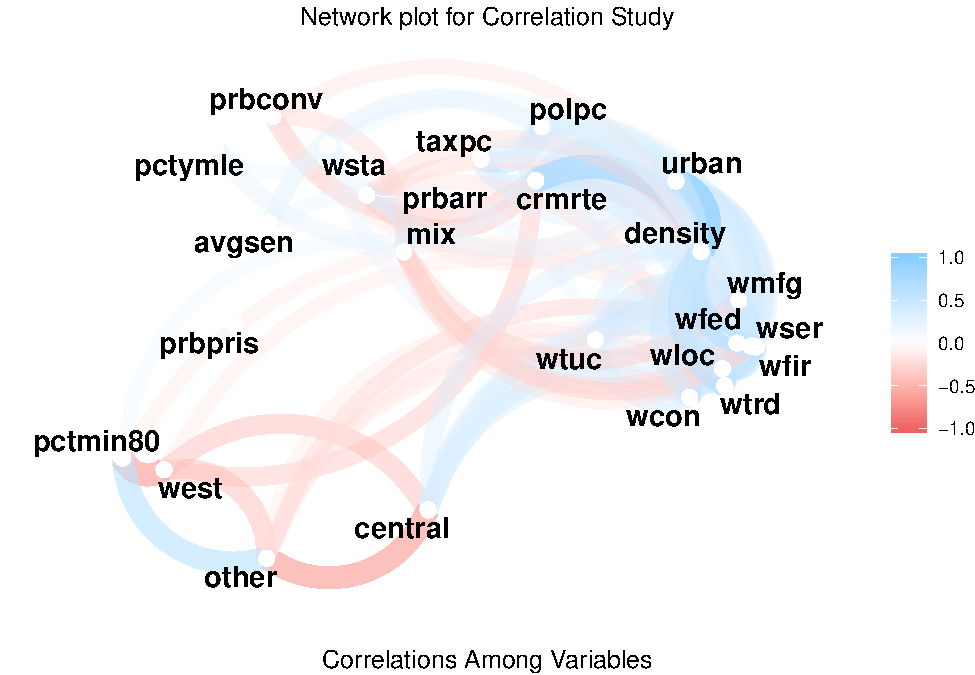
\includegraphics{Bagnard_Gaustad_Hartman_Leung_Lab_3_files/figure-latex/unnamed-chunk-43-1.pdf}
First, we note the general proximity of variables with one another.
Variables that are clustered together represent the overall magnitude of
their correlations. In fact, the cluster of the wage variables are an
indication of very tight correlation. Only state wages fall outside this
group. The telecom and utlity wage variable, while still near the
cluster, show a little relationship.We also see the wage variables are
positively correlated with our crime outcome variable. Density also
positively correlates with wage and the crime rate variable. Urban
correlates with wage, but suprisingly the correlation between crime and
urban is not as high.

Next, we notice the Law enforcement and Judicial variables are clustered
and have a negative correlation with our outcome variable on crime. We
also see they tend to be negatively correlated among one another. For
example, probability of conviction is slightly negatively corrrelated
with the probability of arrest, and both are negatively correlated with
our outcome variable. We also see that police per capita and tax per
capita are positively correlated with another. This makes sense as the
more revenues collected the higher the ability to pay for law
enforcement and protection. Both are also positively correlated with our
outcome variable on crime. We also notice that percent young male has a
positive correlation with crime rate. A possible explanation for this is
that more crimes are committed by younger men as a whole. We also note
that the state wage variable is in nearby proximity.

The mix variable is an odd one. It is possitively correlated with
probability of arrests, negatively correlated with probability of
convictions, and negatively correlated with service and manufacturing
wages. It also has a slight positive correlation with the state wage
variable and seems to be clustered with it.

Last, we turn to our region variables and notice the high negative
correlation of the minority variable with the western region dummy
variable. We also notice a high positive corrlation of minorities with
the `other' (coastal) dummy variable. The pctmin80 variable also
correlates positively with crime rate, although the two are not
clustered. We especially note that west is negatively correlated with
crime rate. There appears to be a lessor propensity for crime in this
region, or perhaps a lack of suffient means to detect it. For a futher
examination of correlation plots for each of the regions please see the
network diagrams in the appendix.

\hypertarget{additional-variables-to-operationalize}{%
\subsection{Additional Variables to
Operationalize}\label{additional-variables-to-operationalize}}

As a final point of discussion we will identify variables we wish to
operationalize for use in our models. We will include a variable that
expresses the economic condition of the county and a variable that
expresses criminal justice effectiveness.

The first variable on the economic condition will include the sum of all
average weekly wages from the 1980 census information. Since we do not
know how many were employed at that wage we use this summary the best
available proxy. Additionally, we will scale this wage variable by 9 to
highlight indication of industry diversity within a county.

\begin{Shaded}
\begin{Highlighting}[]
\NormalTok{dfCrime}\OperatorTok{$}\NormalTok{scaledWages<-(dfCrime}\OperatorTok{$}\NormalTok{wcon }\OperatorTok{+}\StringTok{ }\NormalTok{dfCrime}\OperatorTok{$}\NormalTok{wtuc }\OperatorTok{+}\StringTok{ }\NormalTok{dfCrime}\OperatorTok{$}\NormalTok{wtrd }\OperatorTok{+}\StringTok{ }\NormalTok{dfCrime}\OperatorTok{$}\NormalTok{wfir }\OperatorTok{+}
\StringTok{    }\NormalTok{dfCrime}\OperatorTok{$}\NormalTok{wser }\OperatorTok{+}\StringTok{ }\NormalTok{dfCrime}\OperatorTok{$}\NormalTok{wmfg }\OperatorTok{+}\StringTok{ }\NormalTok{dfCrime}\OperatorTok{$}\NormalTok{wfed }\OperatorTok{+}\StringTok{ }\NormalTok{dfCrime}\OperatorTok{$}\NormalTok{wsta }\OperatorTok{+}\StringTok{ }\NormalTok{dfCrime}\OperatorTok{$}\NormalTok{wloc) }\OperatorTok{/}\StringTok{ }\DecValTok{9}
\end{Highlighting}
\end{Shaded}

As a second variable, we are interested in understanding the
effectiveness of the criminal justice system as a crime deterrent. Our
proxy will be the number of convictions per incident.

This is operationalized by taking the probability of arrests, pbrarr
(which is defined as arrests per incident) and multiplying by the
probability of convictions, pbrconv (which is defined as convictions per
arrest). The new variable is defined below.

\begin{Shaded}
\begin{Highlighting}[]
\NormalTok{dfCrime}\OperatorTok{$}\NormalTok{crimJustEff<-dfCrime}\OperatorTok{$}\NormalTok{prbarr }\OperatorTok{*}\StringTok{ }\NormalTok{dfCrime}\OperatorTok{$}\NormalTok{prbconv}
\end{Highlighting}
\end{Shaded}

We will also create a logarithmic transformation of this variable based
on our histogram analysis from before.

\begin{Shaded}
\begin{Highlighting}[]
\NormalTok{dfCrime}\OperatorTok{$}\NormalTok{logcrimJustEff<-}\KeywordTok{log}\NormalTok{(dfCrime}\OperatorTok{$}\NormalTok{crimJustEff)}
\end{Highlighting}
\end{Shaded}

\hypertarget{summary-and-results}{%
\subsection{Summary and Results}\label{summary-and-results}}

Our outcome variable is the \emph{crime rate} (``crmrte''), which is
defined as the crimes committed per person in a specific county during
1987. The crime rate of the 90 counties in our sample dataset range
between 0.0055 - 0.0990, with a mean of 0.0335.

From the boxplot below, most of the counties have a crime rate between
0.0055 and 0.0700, with 5 outliers having a crime rate \textgreater{}
0.0700.

\begin{Shaded}
\begin{Highlighting}[]
\NormalTok{p<-}\KeywordTok{ggplot}\NormalTok{(}\DataTypeTok{data =}\NormalTok{ dfCrime, }\KeywordTok{aes}\NormalTok{(}\DataTypeTok{y =}\NormalTok{ crmrte, }\DataTypeTok{color =}\NormalTok{ regcode)) }\OperatorTok{+}\StringTok{ }
\StringTok{     }\KeywordTok{geom_boxplot}\NormalTok{() }\OperatorTok{+}\StringTok{ }\KeywordTok{facet_wrap}\NormalTok{(}\OperatorTok{~}\StringTok{ }\NormalTok{regcode)}
\NormalTok{p2<-}\KeywordTok{ggplot}\NormalTok{(}\DataTypeTok{data =}\NormalTok{ dfCrime, }\KeywordTok{aes}\NormalTok{(}\DataTypeTok{y =}\NormalTok{ crmrte)) }\OperatorTok{+}
\StringTok{     }\KeywordTok{geom_boxplot}\NormalTok{()}

\KeywordTok{grid.arrange}\NormalTok{(p, p2, }\DataTypeTok{ncol=}\DecValTok{2}\NormalTok{)}
\end{Highlighting}
\end{Shaded}

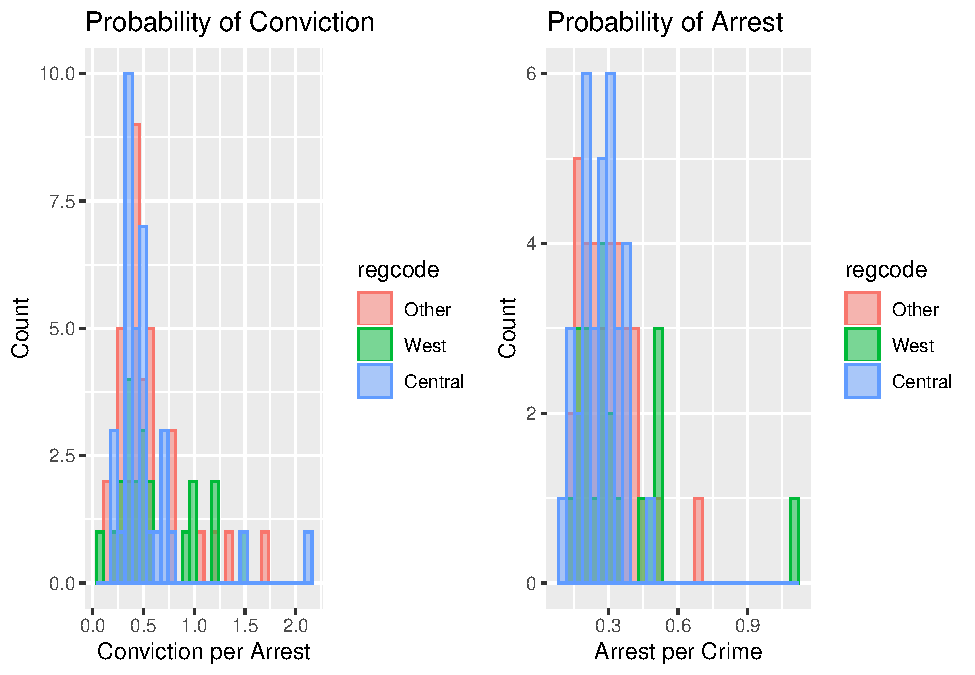
\includegraphics{Bagnard_Gaustad_Hartman_Leung_Lab_3_files/figure-latex/unnamed-chunk-47-1.pdf}

\begin{Shaded}
\begin{Highlighting}[]
\KeywordTok{options}\NormalTok{(}\DataTypeTok{repr.plot.width=}\DecValTok{3}\NormalTok{, }\DataTypeTok{repr.plot.height=}\DecValTok{4}\NormalTok{)}
\KeywordTok{ggplot}\NormalTok{(}\DataTypeTok{data =}\NormalTok{ dfCrime, }\KeywordTok{aes}\NormalTok{(}\DataTypeTok{y =}\NormalTok{ crmrte)) }\OperatorTok{+}\StringTok{ }
\StringTok{      }\KeywordTok{geom_boxplot}\NormalTok{()}
\end{Highlighting}
\end{Shaded}

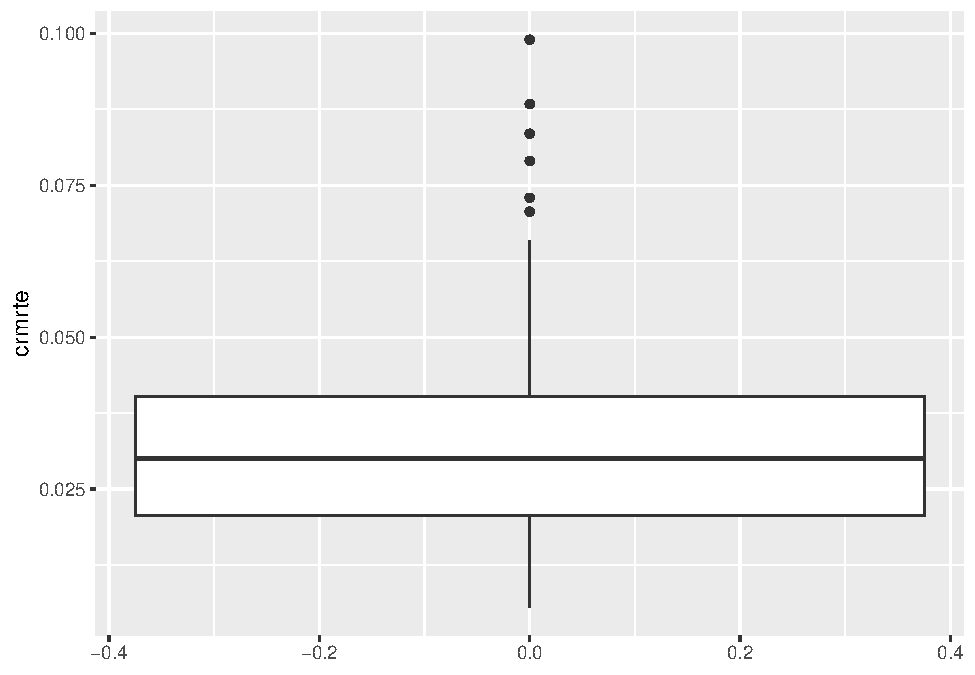
\includegraphics{Bagnard_Gaustad_Hartman_Leung_Lab_3_files/figure-latex/unnamed-chunk-48-1.pdf}

While mix (the type of crime committed) is also potentially an outcome
variable, our research focuses on providing policy recommendations to
reduce crime in general and not a specific type of crime. Mix is also
not a linear outcome and hence difficult to measure.

We propose 3 multiple linear regression models

\begin{itemize}
\item
  First Model: Has only the explanatory variables of key interest and no
  other covariates.
\item
  Second Model: Includes the explanatory variables and covariates that
  increase the accuracy of our results without substantial bias.
\item
  Third Model: An expansion of the second model with most covariates,
  designed to demonstrate the robustness of our results to model
  specification.
\end{itemize}

As we proceed with each model, we verify the CLM assumptions of OLS are
addressed below:

\begin{itemize}
\item
  \textbf{MLR1} Linear in parameters: The models have had its data
  transformed as described above to allow a linear fit of the model.
\item
  \textbf{MLR2} Random Sampling: The data is collected from a data set
  with rolled up data for each county. It is not randomly sampled by
  area or population.
\item
  \textbf{MLR3} to be discussed on a model by model basis.
\item
  \textbf{MLR4} to be discussed on a model by model basis.
\item
  \textbf{MLR5'} to be discussed on a model by model basis.
\item
  \textbf{MLR6'} to be discussed on a model by model basis.
\end{itemize}

By satisfying these assumptions, we can expect our coefficients will be
approaching the true parameter values in probability.

\hypertarget{model-analysis}{%
\section{Model Analysis}\label{model-analysis}}

\hypertarget{model-1}{%
\subsection{Model 1}\label{model-1}}

\hypertarget{introduction-1}{%
\subsubsection{Introduction}\label{introduction-1}}

Our base hypothesis is that county level crime can be fundamentally
explained by three factors: the geographical region of the county, the
effectiveness of the criminal justice system, and economic conditions in
the county.

\begin{itemize}
\tightlist
\item
  \textbf{Criminal Justice Effectiveness}\\
  Criminal Justice Effectiveness is an abstract concept that is
  operationalized by comparing the number of crimes to convictions. To
  track crimes, they must be reported to police, who can then make
  arrests. Then, the legal system provides judgement in the form of
  convictions and sentencing. Besides removing some criminals from
  society, criminal justice can serve as deterrent, as the probability
  of getting caught, convicted, sentenced could discourage some would be
  criminals from committing crimes.
\end{itemize}

We operationalize criminal justice effectiveness as (probability of
Convictions * Crimes committed). We define this as: prbconv * prbarr =
conv/arrest * arrest/crime = convictions/crime. Without more granular
data, this provides a single parsimonious metric that helps understand
how well the law enforcement and criminal justice system works.

\begin{itemize}
\item
  \textbf{Region}\\
  Region is easily identified as possible factor for predicting crime as
  seen from our initial EDA in the Introduction. It would be expected
  that cultural, econocomic, government, geographic, and demographic
  profiles among other important variables would vary across the
  regions. Without the ability to measure and operationalize these
  variables, region offers a solid standin.
\item
  \textbf{Economic Conditions} Finally, we theorize that the third major
  cause of crime are economic conditions. We would expect that as
  someone's economic success and opportunity increases their propensity
  to commit crime is lowered. And similarly when there are worse
  economic conditions, crime would increase due to lack of means, lack
  of occupation or boredom. This also means that individuals have less
  to look forward to and are willing to risk their freedom or endanger
  themselves.
\end{itemize}

We operationalize economic conditions by looking at wages. For this
base, parsimonious model, we define this as the unweighted average
weekly pay from each sector provided in the data set. We think this is
best proxy from our data because it answers all of the above (higher
wages leads to better means and better opportunities). From our EDA we
also confirm that in general these sums are not skewed by having 1
really high paying sector in each county as we see a strong relationship
between average quartile across all job types and unweighted sector
average wage. This can be seen in the chart below.

\hypertarget{model-1-eda}{%
\subsubsection{Model 1 EDA}\label{model-1-eda}}

\textbf{Data Transformations: Criminal Justice Effectiveness} First we
look at the components of the Criminal Justice Effectiveness:
Probability of arrest and Probability of conviction.

\begin{Shaded}
\begin{Highlighting}[]
\NormalTok{p1 <-}\StringTok{ }\KeywordTok{ggplot}\NormalTok{(dfCrime, }\KeywordTok{aes}\NormalTok{(}\DataTypeTok{x =}\NormalTok{ prbarr, }\DataTypeTok{color=}\NormalTok{regcode, }\DataTypeTok{fill =}\NormalTok{ regcode)) }\OperatorTok{+}\StringTok{ }
\StringTok{  }\KeywordTok{geom_histogram}\NormalTok{(}\DataTypeTok{position=}\StringTok{"identity"}\NormalTok{, }\DataTypeTok{alpha=}\FloatTok{0.5}\NormalTok{, }\DataTypeTok{bins=}\DecValTok{30}\NormalTok{) }\OperatorTok{+}
\StringTok{  }\KeywordTok{labs}\NormalTok{(}\DataTypeTok{title=}\StringTok{"Probability of Arrest"}\NormalTok{, }\DataTypeTok{x=}\StringTok{"Arrest per Crime"}\NormalTok{, }\DataTypeTok{y=}\StringTok{"Count"}\NormalTok{)}
\NormalTok{p2 <-}\StringTok{ }\KeywordTok{ggplot}\NormalTok{(dfCrime, }\KeywordTok{aes}\NormalTok{(}\DataTypeTok{x =}\NormalTok{ prbconv, }\DataTypeTok{color=}\NormalTok{regcode, }\DataTypeTok{fill =}\NormalTok{ regcode)) }\OperatorTok{+}\StringTok{ }
\StringTok{  }\KeywordTok{geom_histogram}\NormalTok{(}\DataTypeTok{position=}\StringTok{"identity"}\NormalTok{, }\DataTypeTok{alpha=}\FloatTok{0.5}\NormalTok{, }\DataTypeTok{bins=}\DecValTok{30}\NormalTok{) }\OperatorTok{+}
\StringTok{  }\KeywordTok{labs}\NormalTok{(}\DataTypeTok{title=}\StringTok{"Probability of Conviction"}\NormalTok{, }\DataTypeTok{x=}\StringTok{"Conviction per Arrest"}\NormalTok{, }\DataTypeTok{y=}\StringTok{"Count"}\NormalTok{)}
\KeywordTok{grid.arrange}\NormalTok{(p2, p1, }\DataTypeTok{ncol=}\DecValTok{2}\NormalTok{)}
\end{Highlighting}
\end{Shaded}

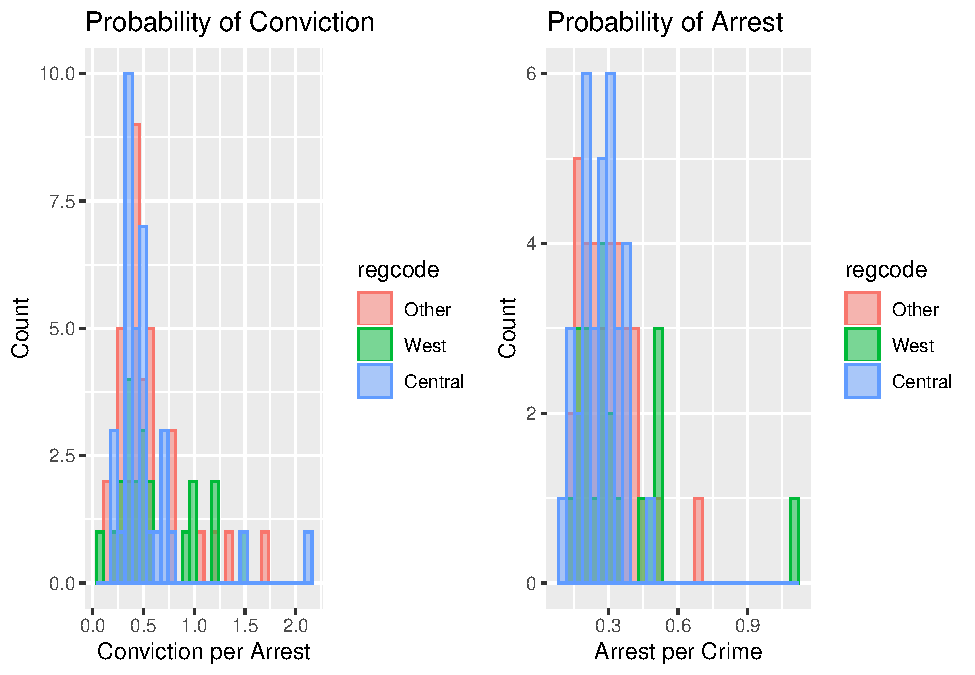
\includegraphics{Bagnard_Gaustad_Hartman_Leung_Lab_3_files/figure-latex/unnamed-chunk-49-1.pdf}

The distribution of both probability of conviction and probability of
arrest are skewed right. It could be argued that both of these variables
should be bound between 0 and 1. However, these ``probabilities'' are
proxied by ratios. It is in fact possible (and perhaps common) that
defendents are charged with multiple crimes and convicted, but were only
arrested once. For this reason we will not consider outliers in this
variable.

For ``probability'' of arrest, it could be possible there are multiple
arrests for a single crime. However, the single data point that is
greater than one, is \textgreater{}5 standard deviations away from the
distribution. Since this value falls so far out of distribution, it will
have high leverage on our model and will be preemptively imputed as the
data supplied is likely in error and is not representative of the bulk
of North Carolina counties.

\begin{Shaded}
\begin{Highlighting}[]
\CommentTok{# how many standard deviations away the outlier lies}
\NormalTok{(dfCrime[}\DecValTok{51}\NormalTok{,]}\OperatorTok{$}\NormalTok{prbarr }\OperatorTok{-}\StringTok{ }\KeywordTok{mean}\NormalTok{(dfCrime}\OperatorTok{$}\NormalTok{prbarr))}\OperatorTok{/}\KeywordTok{sd}\NormalTok{(dfCrime}\OperatorTok{$}\NormalTok{prbarr) }\CommentTok{# standard deviations away from the mean.}
\end{Highlighting}
\end{Shaded}

\begin{verbatim}
[1] 5.779438
\end{verbatim}

We will use the imputation method to replace the large prbarr value and
remove the outlier effect, while also retaining the rest of the
variables in the county.

\begin{Shaded}
\begin{Highlighting}[]
\NormalTok{dfCrime[dfCrime}\OperatorTok{$}\NormalTok{crimJustEff }\OperatorTok{>}\StringTok{ }\DecValTok{1}\NormalTok{,] }\CommentTok{# find outlier}
\end{Highlighting}
\end{Shaded}

\begin{verbatim}
   county year    crmrte  prbarr prbconv prbpris avgsen       polpc
51    115   87 0.0055332 1.09091     1.5     0.5   20.7 0.002624843
     density   taxpc west central urban  pctmin80     wcon     wtuc
51 0.3858093 28.1931    1       0     0 0.0128365 204.2206 503.2351
       wtrd     wfir     wser   wmfg  wfed   wsta   wloc mix    pctymle
51 217.4908 342.4658 245.2061 448.42 442.2 340.39 386.12 0.1 0.07253495
   region regcode other nonurban         metro scaledWages crimJustEff
51      1    West     0        1 Outside Metro    347.7498    1.636365
   logcrimJustEff
51      0.4924773
\end{verbatim}

We will use the imputation method to remove the outlier effect in this
record while retaining the remaining observations from the county.

\begin{Shaded}
\begin{Highlighting}[]
\NormalTok{dfCrime}\OperatorTok{$}\NormalTok{prbarr[}\KeywordTok{which}\NormalTok{(dfCrime}\OperatorTok{$}\NormalTok{county}\OperatorTok{==}\DecValTok{115}\NormalTok{)]<-}\OtherTok{NA} \CommentTok{# set the value to NA so it will be imputed}
\end{Highlighting}
\end{Shaded}

\begin{Shaded}
\begin{Highlighting}[]
\NormalTok{impute_arg <-}\StringTok{ }\KeywordTok{aregImpute}\NormalTok{(}\OperatorTok{~}\StringTok{ }\NormalTok{crmrte }\OperatorTok{+}\StringTok{  }\NormalTok{urban }\OperatorTok{+}\StringTok{ }\NormalTok{central }\OperatorTok{+}\StringTok{ }\NormalTok{west }\OperatorTok{+}\StringTok{ }\NormalTok{other }\OperatorTok{+}
\StringTok{                         }\NormalTok{prbarr }\OperatorTok{+}\StringTok{ }\NormalTok{prbconv }\OperatorTok{+}\StringTok{ }\NormalTok{prbpris }\OperatorTok{+}\StringTok{ }\NormalTok{avgsen }\OperatorTok{+}\StringTok{ }\NormalTok{polpc }\OperatorTok{+}\StringTok{ }
\StringTok{                         }\NormalTok{density }\OperatorTok{+}\StringTok{ }\NormalTok{taxpc }\OperatorTok{+}\StringTok{ }\NormalTok{pctmin80 }\OperatorTok{+}\StringTok{ }\NormalTok{wcon }\OperatorTok{+}\StringTok{ }\NormalTok{wtuc }\OperatorTok{+}
\StringTok{                         }\NormalTok{wtrd }\OperatorTok{+}\StringTok{ }\NormalTok{wfir }\OperatorTok{+}\StringTok{ }\NormalTok{wser }\OperatorTok{+}\StringTok{ }\NormalTok{wmfg }\OperatorTok{+}\StringTok{ }\NormalTok{wfed }\OperatorTok{+}\StringTok{ }\NormalTok{wsta }\OperatorTok{+}\StringTok{ }\NormalTok{wloc }\OperatorTok{+}
\StringTok{                         }\NormalTok{mix }\OperatorTok{+}\StringTok{ }\NormalTok{pctymle, }\DataTypeTok{data =}\NormalTok{ dfCrime, }\DataTypeTok{match=}\StringTok{"weighted"}\NormalTok{,}
                         \DataTypeTok{nk=}\DecValTok{3}\NormalTok{, }\DataTypeTok{B=}\DecValTok{10}\NormalTok{, }\DataTypeTok{n.impute =} \DecValTok{100}\NormalTok{)}
\end{Highlighting}
\end{Shaded}

\begin{Shaded}
\begin{Highlighting}[]
\KeywordTok{paste}\NormalTok{(}\StringTok{"R-squares for Predicting Non-Missing Values for Each Variable"}\NormalTok{)}
\end{Highlighting}
\end{Shaded}

\begin{verbatim}
[1] "R-squares for Predicting Non-Missing Values for Each Variable"
\end{verbatim}

\begin{Shaded}
\begin{Highlighting}[]
\NormalTok{impute_arg}\OperatorTok{$}\NormalTok{rsq}
\end{Highlighting}
\end{Shaded}

\begin{verbatim}
   prbarr 
0.9309518 
\end{verbatim}

\begin{Shaded}
\begin{Highlighting}[]
\KeywordTok{paste}\NormalTok{(}\StringTok{"Predicted values"}\NormalTok{)}
\end{Highlighting}
\end{Shaded}

\begin{verbatim}
[1] "Predicted values"
\end{verbatim}

\begin{Shaded}
\begin{Highlighting}[]
\KeywordTok{mean}\NormalTok{(impute_arg}\OperatorTok{$}\NormalTok{imputed}\OperatorTok{$}\NormalTok{prbarr)}
\end{Highlighting}
\end{Shaded}

\begin{verbatim}
[1] 0.3633065
\end{verbatim}

We will reassign this value using the mean from the trials.

\begin{Shaded}
\begin{Highlighting}[]
\NormalTok{dfCrime}\OperatorTok{$}\NormalTok{prbarr[}\KeywordTok{which}\NormalTok{(dfCrime}\OperatorTok{$}\NormalTok{county}\OperatorTok{==}\DecValTok{115}\NormalTok{)]<-}\KeywordTok{mean}\NormalTok{(impute_arg}\OperatorTok{$}\NormalTok{imputed}\OperatorTok{$}\NormalTok{prbarr)}
\end{Highlighting}
\end{Shaded}

With the outlier imputed. The Criminal Justice Effectiveness can be
constructed as described above. And a histogram can show how log
transformation improves normality. Also, by log transforming we can
understand the resulting coefficient as a percent change in the ratio of
Criminal Justice Effectiveness (convictions/crime).

\begin{Shaded}
\begin{Highlighting}[]
\NormalTok{dfCrime}\OperatorTok{$}\NormalTok{crimJustEff<-dfCrime}\OperatorTok{$}\NormalTok{prbarr }\OperatorTok{*}\StringTok{ }\NormalTok{dfCrime}\OperatorTok{$}\NormalTok{prbconv}
\NormalTok{dfCrime}\OperatorTok{$}\NormalTok{logcrimJustEff<-}\KeywordTok{log}\NormalTok{(dfCrime}\OperatorTok{$}\NormalTok{crimJustEff)}
\NormalTok{dfCrime}\OperatorTok{$}\NormalTok{logcrmrte <-}\StringTok{ }\KeywordTok{log}\NormalTok{(dfCrime}\OperatorTok{$}\NormalTok{crmrte)}
\KeywordTok{options}\NormalTok{(}\DataTypeTok{repr.plot.width=}\DecValTok{4}\NormalTok{, }\DataTypeTok{repr.plot.height=}\DecValTok{4}\NormalTok{)}
\NormalTok{p1 <-}\StringTok{ }\KeywordTok{ggplot}\NormalTok{(dfCrime, }\KeywordTok{aes}\NormalTok{(}\DataTypeTok{x =}\NormalTok{ crimJustEff, }\DataTypeTok{color=}\NormalTok{regcode, }\DataTypeTok{fill =}\NormalTok{ regcode)) }\OperatorTok{+}\StringTok{ }
\StringTok{  }\KeywordTok{geom_histogram}\NormalTok{(}\DataTypeTok{position=}\StringTok{"identity"}\NormalTok{, }\DataTypeTok{alpha=}\FloatTok{0.5}\NormalTok{, }\DataTypeTok{bins=}\DecValTok{30}\NormalTok{) }\OperatorTok{+}
\StringTok{  }\KeywordTok{labs}\NormalTok{(}\DataTypeTok{title=}\StringTok{"Criminal Justice Effectiveness"}\NormalTok{, }\DataTypeTok{x=}\StringTok{"Convictions per Crime"}\NormalTok{, }\DataTypeTok{y=}\StringTok{"Count"}\NormalTok{)}
\NormalTok{p2 <-}\StringTok{ }\KeywordTok{ggplot}\NormalTok{(dfCrime, }\KeywordTok{aes}\NormalTok{(}\DataTypeTok{x =}\NormalTok{ logcrimJustEff, }\DataTypeTok{color=}\NormalTok{regcode, }\DataTypeTok{fill =}\NormalTok{ regcode)) }\OperatorTok{+}\StringTok{ }
\StringTok{  }\KeywordTok{geom_histogram}\NormalTok{(}\DataTypeTok{position=}\StringTok{"identity"}\NormalTok{, }\DataTypeTok{alpha=}\FloatTok{0.5}\NormalTok{, }\DataTypeTok{bins=}\DecValTok{30}\NormalTok{) }\OperatorTok{+}
\StringTok{  }\KeywordTok{labs}\NormalTok{(}\DataTypeTok{title=}\StringTok{"log(Criminal Justice Effectiveness)"}\NormalTok{, }\DataTypeTok{x=}\StringTok{"log(Convictions per Crime)"}\NormalTok{, }\DataTypeTok{y=}\StringTok{"Count"}\NormalTok{)}
\KeywordTok{grid.arrange}\NormalTok{(p1, p2, }\DataTypeTok{ncol=}\DecValTok{2}\NormalTok{)}
\end{Highlighting}
\end{Shaded}

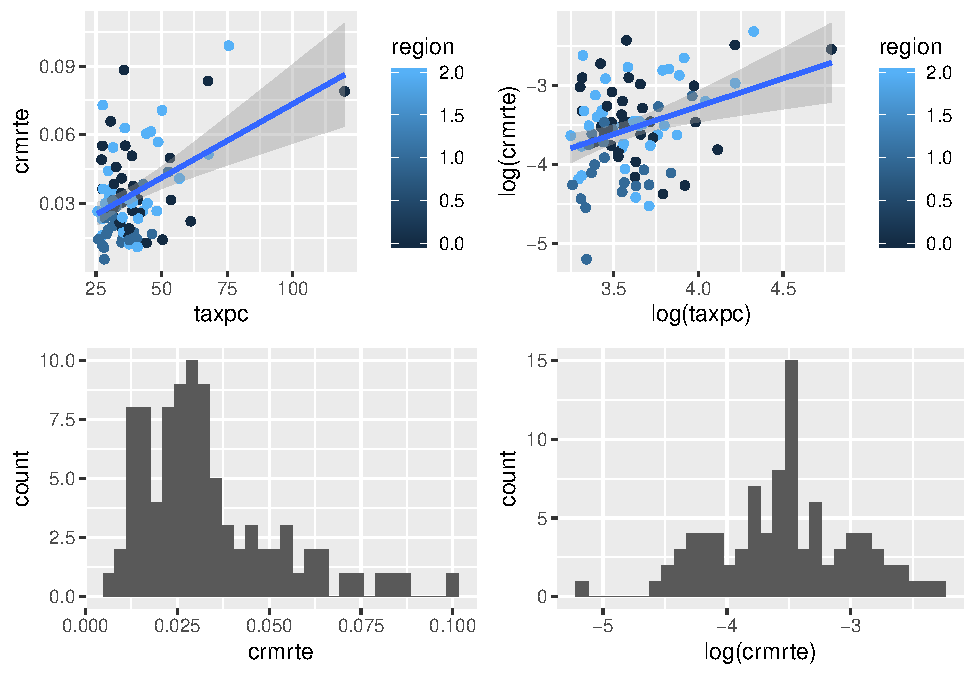
\includegraphics{Bagnard_Gaustad_Hartman_Leung_Lab_3_files/figure-latex/unnamed-chunk-56-1.pdf}

\textbf{Data Transformations: Unweighted Average of Sector Wages}

Now we turn our attention to the economic variable, unweighted average
wage of all provided sectors. The wages trend together well, so there is
limited information lost when combining them into one variable. This can
be seen by plotting quartiles of each wage against the unweighted
average and observing a relatively linear response.

\begin{Shaded}
\begin{Highlighting}[]
\CommentTok{# # Quantiles for all jobs}
\NormalTok{dfWage<-}\KeywordTok{mutate}\NormalTok{(dfCrime,}\DataTypeTok{qCon=}\KeywordTok{ntile}\NormalTok{(dfCrime}\OperatorTok{$}\NormalTok{wcon,}\DecValTok{4}\NormalTok{))}
\NormalTok{dfWage<-}\KeywordTok{mutate}\NormalTok{(dfWage,}\DataTypeTok{qTuc=}\KeywordTok{ntile}\NormalTok{(dfCrime}\OperatorTok{$}\NormalTok{wtuc,}\DecValTok{4}\NormalTok{))}
\NormalTok{dfWage<-}\KeywordTok{mutate}\NormalTok{(dfWage,}\DataTypeTok{qTrd=}\KeywordTok{ntile}\NormalTok{(dfCrime}\OperatorTok{$}\NormalTok{wtrd,}\DecValTok{4}\NormalTok{))}
\NormalTok{dfWage<-}\KeywordTok{mutate}\NormalTok{(dfWage,}\DataTypeTok{qFir=}\KeywordTok{ntile}\NormalTok{(dfCrime}\OperatorTok{$}\NormalTok{wfir,}\DecValTok{4}\NormalTok{))}
\NormalTok{dfWage<-}\KeywordTok{mutate}\NormalTok{(dfWage,}\DataTypeTok{qSer=}\KeywordTok{ntile}\NormalTok{(dfCrime}\OperatorTok{$}\NormalTok{wser,}\DecValTok{4}\NormalTok{))}
\NormalTok{dfWage<-}\KeywordTok{mutate}\NormalTok{(dfWage,}\DataTypeTok{qMfg=}\KeywordTok{ntile}\NormalTok{(dfCrime}\OperatorTok{$}\NormalTok{wmfg,}\DecValTok{4}\NormalTok{))}
\NormalTok{dfWage<-}\KeywordTok{mutate}\NormalTok{(dfWage,}\DataTypeTok{qFed=}\KeywordTok{ntile}\NormalTok{(dfCrime}\OperatorTok{$}\NormalTok{wfed,}\DecValTok{4}\NormalTok{))}
\NormalTok{dfWage<-}\KeywordTok{mutate}\NormalTok{(dfWage,}\DataTypeTok{qSta=}\KeywordTok{ntile}\NormalTok{(dfCrime}\OperatorTok{$}\NormalTok{wsta,}\DecValTok{4}\NormalTok{))}
\NormalTok{dfWage<-}\KeywordTok{mutate}\NormalTok{(dfWage,}\DataTypeTok{qLoc=}\KeywordTok{ntile}\NormalTok{(dfCrime}\OperatorTok{$}\NormalTok{wloc,}\DecValTok{4}\NormalTok{))}
\CommentTok{## Average quantile}
\NormalTok{dfWage}\OperatorTok{$}\NormalTok{qAvg=}\StringTok{ }\NormalTok{(dfWage}\OperatorTok{$}\NormalTok{qCon}\OperatorTok{+}\NormalTok{dfWage}\OperatorTok{$}\NormalTok{qTuc}\OperatorTok{+}\NormalTok{dfWage}\OperatorTok{$}\NormalTok{qTrd}\OperatorTok{+}\NormalTok{dfWage}\OperatorTok{$}\NormalTok{qFir}\OperatorTok{+}\NormalTok{dfWage}\OperatorTok{$}\NormalTok{qSer}\OperatorTok{+}\NormalTok{dfWage}\OperatorTok{$}\NormalTok{qMfg}\OperatorTok{+}
\StringTok{                }\NormalTok{dfWage}\OperatorTok{$}\NormalTok{qFed}\OperatorTok{+}\NormalTok{dfWage}\OperatorTok{$}\NormalTok{qSta}\OperatorTok{+}\NormalTok{dfWage}\OperatorTok{$}\NormalTok{qLoc)}\OperatorTok{/}\DecValTok{9}

\CommentTok{#plot(dfCrime$scaledWages,dfWage$qAvg)}
\CommentTok{#ggplot( aes(x = dfCrime$scaledWages, y = dfWage$qAvg)) + }
\CommentTok{#      geom_point()+}
\CommentTok{#  geom_smooth(method = "lm")}
\end{Highlighting}
\end{Shaded}

We will again modify this variable with a log transformation for better
interpretation. This allows us to interpret percent changes in wage
which is more consistent across a range of wages. The result is a
relatively normal distribution as seen in the below histogram. There
exists a small ``second mode'' for a few of the central region counties.

\begin{Shaded}
\begin{Highlighting}[]
\NormalTok{dfCrime}\OperatorTok{$}\NormalTok{logScaledWages <-}\StringTok{ }\KeywordTok{log}\NormalTok{(dfCrime}\OperatorTok{$}\NormalTok{scaledWages)}
\NormalTok{p1 <-}\StringTok{ }\KeywordTok{ggplot}\NormalTok{(dfCrime, }\KeywordTok{aes}\NormalTok{(}\DataTypeTok{x =}\NormalTok{ logScaledWages, }\DataTypeTok{color=}\NormalTok{regcode, }\DataTypeTok{fill =}\NormalTok{ regcode)) }\OperatorTok{+}\StringTok{ }
\StringTok{  }\KeywordTok{geom_histogram}\NormalTok{(}\DataTypeTok{position=}\StringTok{"identity"}\NormalTok{, }\DataTypeTok{alpha=}\FloatTok{0.5}\NormalTok{, }\DataTypeTok{bins=}\DecValTok{30}\NormalTok{) }\OperatorTok{+}
\StringTok{  }\KeywordTok{labs}\NormalTok{(}\DataTypeTok{title=}\StringTok{"log(Scaled Wages)"}\NormalTok{, }\DataTypeTok{x=}\StringTok{"log(Scaled Wages)"}\NormalTok{, }\DataTypeTok{y=}\StringTok{"Count"}\NormalTok{)}
\NormalTok{p1}
\end{Highlighting}
\end{Shaded}

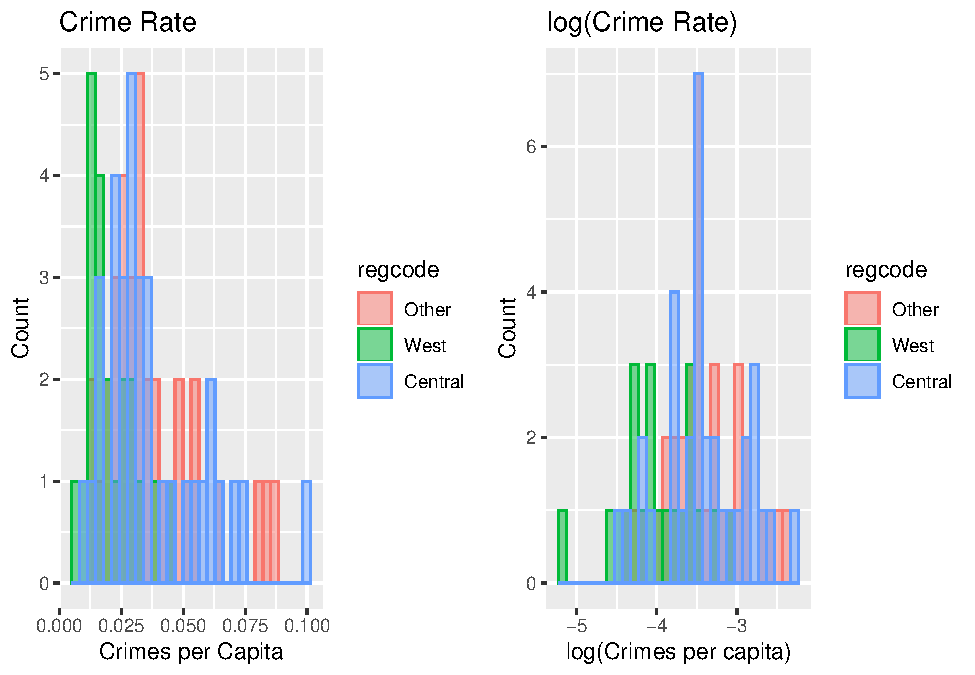
\includegraphics{Bagnard_Gaustad_Hartman_Leung_Lab_3_files/figure-latex/unnamed-chunk-58-1.pdf}
Interestingly, when viewing the wage data plotted against crime rate
(below). We see that there is a positive correlation between wages and
crime. We will see if this holds when taking into account the Criminal
Justice Effectiveness in model 1 and discuss some possible causes.

\begin{Shaded}
\begin{Highlighting}[]
\NormalTok{q9<-}\KeywordTok{ggplot}\NormalTok{(}\DataTypeTok{data =}\NormalTok{ dfCrime, }\KeywordTok{aes}\NormalTok{(}\DataTypeTok{x =}\NormalTok{ logScaledWages, }\DataTypeTok{y =}\NormalTok{ logcrmrte, }\DataTypeTok{color =}\NormalTok{ regcode)) }\OperatorTok{+}\StringTok{ }
\StringTok{      }\KeywordTok{geom_point}\NormalTok{()}\OperatorTok{+}
\StringTok{  }\KeywordTok{geom_smooth}\NormalTok{(}\DataTypeTok{method =} \StringTok{"lm"}\NormalTok{)}
\KeywordTok{options}\NormalTok{(}\DataTypeTok{repr.plot.width=}\DecValTok{8}\NormalTok{, }\DataTypeTok{repr.plot.height=}\DecValTok{16}\NormalTok{)}
\NormalTok{q9}
\end{Highlighting}
\end{Shaded}

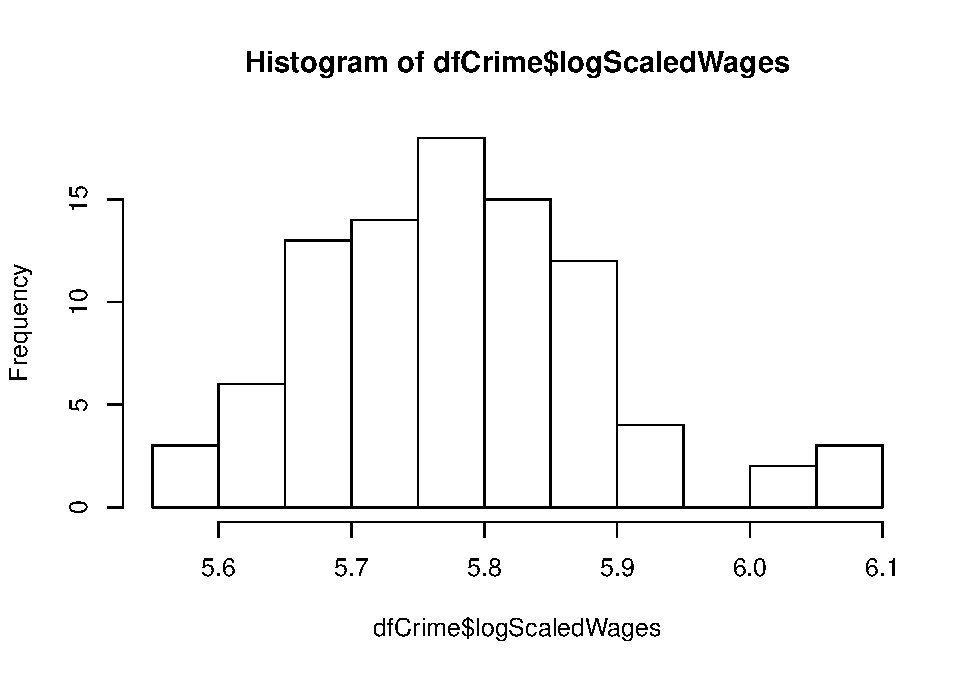
\includegraphics{Bagnard_Gaustad_Hartman_Leung_Lab_3_files/figure-latex/unnamed-chunk-59-1.pdf}

\textbf{Data Transformations: Unweighted Average of Sector Wages}
Finally, regions will be used as explained in the EDA section. No
transformations are necessary.

\hypertarget{model-1-linear-model}{%
\subsubsection{Model 1 Linear Model}\label{model-1-linear-model}}

\[ log(Crime Rate) = B_0 + B_1log(Unweighted Average Wage) + B_2log(Criminal Justice Effectiveness) + B_3Region\]

\begin{Shaded}
\begin{Highlighting}[]
\CommentTok{#dfCrime$unweighted_avg_wage <- dfCrime$scaledWages/9}
\NormalTok{mod1 <-}\StringTok{ }\KeywordTok{lm}\NormalTok{(logcrmrte }\OperatorTok{~}\StringTok{ }\NormalTok{logScaledWages }\OperatorTok{+}\StringTok{ }\NormalTok{logcrimJustEff }\OperatorTok{+}\StringTok{ }\NormalTok{regcode, }\DataTypeTok{data=}\NormalTok{dfCrime)}
\NormalTok{mod1 }\CommentTok{# Coefficients}
\end{Highlighting}
\end{Shaded}

\begin{verbatim}

Call:
lm(formula = logcrmrte ~ logScaledWages + logcrimJustEff + regcode, 
    data = dfCrime)

Coefficients:
   (Intercept)  logScaledWages  logcrimJustEff     regcodeWest  
      -15.8551          1.9981         -0.4795         -0.5896  
regcodeCentral  
       -0.2428  
\end{verbatim}

\begin{Shaded}
\begin{Highlighting}[]
\KeywordTok{summary}\NormalTok{(mod1)}\OperatorTok{$}\NormalTok{adj.r.square }\CommentTok{# Adjusted R^2 value.}
\end{Highlighting}
\end{Shaded}

\begin{verbatim}
[1] 0.6360262
\end{verbatim}

\textbf{Cook's Distance (Leverage/Influence) Analysis} None of the
points approach a cook's distance of concern. Some of the higher
leveraged points do trend towards larger negative residuals. This
suggests that our model might not be capturing a phenomenon at more
extreme values of the regressors. For an initial model there is nothing
of major concern.

\begin{Shaded}
\begin{Highlighting}[]
\KeywordTok{plot}\NormalTok{(mod1, }\DataTypeTok{which=}\DecValTok{5}\NormalTok{) }\CommentTok{# Variance Inflation Factor}
\end{Highlighting}
\end{Shaded}

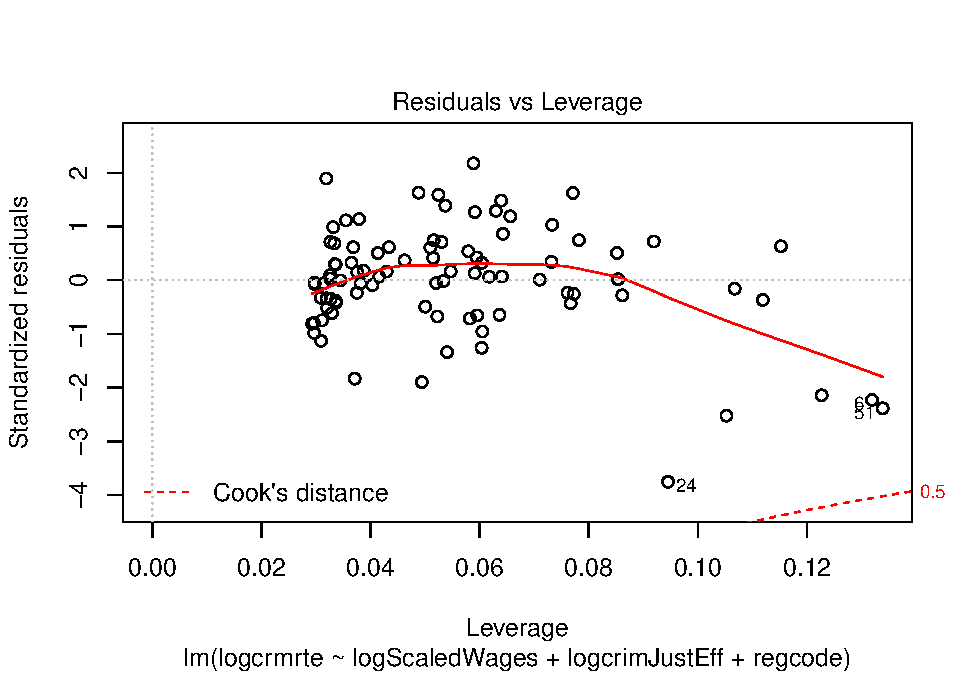
\includegraphics{Bagnard_Gaustad_Hartman_Leung_Lab_3_files/figure-latex/unnamed-chunk-61-1.pdf}

\textbf{Model 1 CLM Assumptions:} * \textbf{MLR1} Linear in parameters:
The model has had its data transformed as described above to allow a
linear fit of the model.

\begin{itemize}
\item
  \textbf{MLR2} Random Sampling: The data is collected from a data set
  with rolled up data for each county. We cannot comment on the
  randomness of the samples, though nearly all counties are represented
  in North Carolina.
\item
  \textbf{MLR3} No perfect multicollinearity: None of the variables
  chosen for the model are constant or perfectly collinear as the
  economy and criminal justice effectiveness are independent. Our low
  VIF value shows very little colinearity, as would be expected from the
  diverse and limited variables included in teh model. .
\end{itemize}

\begin{Shaded}
\begin{Highlighting}[]
\KeywordTok{vif}\NormalTok{(mod1) }\CommentTok{# Variance Inflation Factor}
\end{Highlighting}
\end{Shaded}

\begin{verbatim}
                   GVIF Df GVIF^(1/(2*Df))
logScaledWages 1.205229  1        1.097829
logcrimJustEff 1.048026  1        1.023731
regcode        1.171824  2        1.040436
\end{verbatim}

\begin{itemize}
\item
  \textbf{MLR4'} The expectation of u is 0. This is difficult to prove
  in a data set like this one. It is possible that there are serious
  bias issues in the way crimes are reported and wages. However, if one
  agrees that the data has integrity and that the basic model presented
  for predicting crime rate is acceptable, then exogeneity can be
  accepted.
\item
  \textbf{MLR4} The zero conditional mean assumption is well supported
  when viewing the Residuals vs fitted plot. The spline fit is nearly
  flat and centered very close to zero.
\end{itemize}

\begin{Shaded}
\begin{Highlighting}[]
\KeywordTok{plot}\NormalTok{(mod1, }\DataTypeTok{which=}\DecValTok{1}\NormalTok{)}
\end{Highlighting}
\end{Shaded}

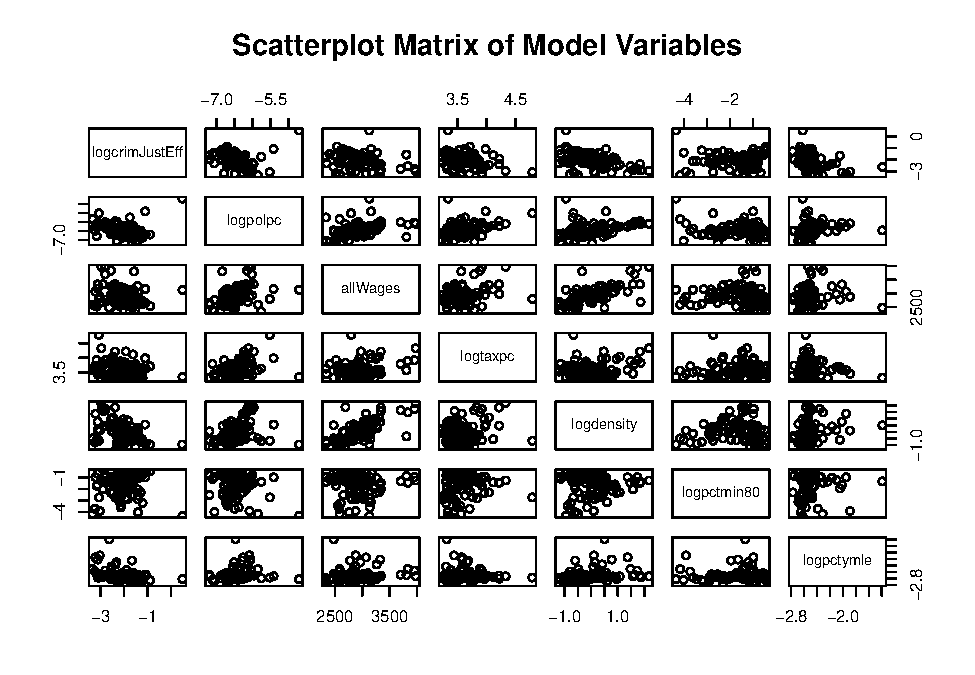
\includegraphics{Bagnard_Gaustad_Hartman_Leung_Lab_3_files/figure-latex/unnamed-chunk-63-1.pdf}

\begin{itemize}
\tightlist
\item
  \textbf{MLR5} There does appear to be heteroskedacity in the `lips'
  appearance of the Residuals vs fitted plot. A Breusch-Pagan test shows
  that there is not heteroskedacity. However, in an effort to limit
  criticism, we will proceed with heteroskedastic robust errors.
\end{itemize}

\begin{Shaded}
\begin{Highlighting}[]
\KeywordTok{bptest}\NormalTok{(mod1)}
\end{Highlighting}
\end{Shaded}

\begin{verbatim}
## 
##  studentized Breusch-Pagan test
## 
## data:  mod1
## BP = 5.232, df = 4, p-value = 0.2643
\end{verbatim}

\begin{Shaded}
\begin{Highlighting}[]
\KeywordTok{coeftest}\NormalTok{(mod1, }\DataTypeTok{vcov=}\NormalTok{vcovHC) }\CommentTok{#coefficients with heteroskedastic consistent standard errors}
\end{Highlighting}
\end{Shaded}

\begin{verbatim}
## 
## t test of coefficients:
## 
##                  Estimate Std. Error t value  Pr(>|t|)    
## (Intercept)    -15.855071   2.660365 -5.9597 5.566e-08 ***
## logScaledWages   1.998057   0.486688  4.1054 9.234e-05 ***
## logcrimJustEff  -0.479533   0.104102 -4.6064 1.427e-05 ***
## regcodeWest     -0.589578   0.101447 -5.8117 1.051e-07 ***
## regcodeCentral  -0.242821   0.081159 -2.9919  0.003628 ** 
## ---
## Signif. codes:  0 '***' 0.001 '**' 0.01 '*' 0.05 '.' 0.1 ' ' 1
\end{verbatim}

\begin{itemize}
\tightlist
\item
  \textbf{MLR6} The final assumption of linear regression is that the
  errors are normally distributed. This appears to hold for the bulk of
  the residuals however there is skewness on the tails. This
  non-normality is also reflected in the significant return on the
  shapiro test. The model should not be used when predicting crime rate
  for counties with values or combinations of the regressors.
\end{itemize}

\begin{Shaded}
\begin{Highlighting}[]
\KeywordTok{shapiro.test}\NormalTok{(mod1}\OperatorTok{$}\NormalTok{residuals) }\CommentTok{# test for normality}
\end{Highlighting}
\end{Shaded}

\begin{verbatim}

    Shapiro-Wilk normality test

data:  mod1$residuals
W = 0.96036, p-value = 0.007719
\end{verbatim}

\begin{Shaded}
\begin{Highlighting}[]
\KeywordTok{plot}\NormalTok{(mod1, }\DataTypeTok{which=}\DecValTok{2}\NormalTok{) }\CommentTok{# QQ plot for residuals}
\end{Highlighting}
\end{Shaded}

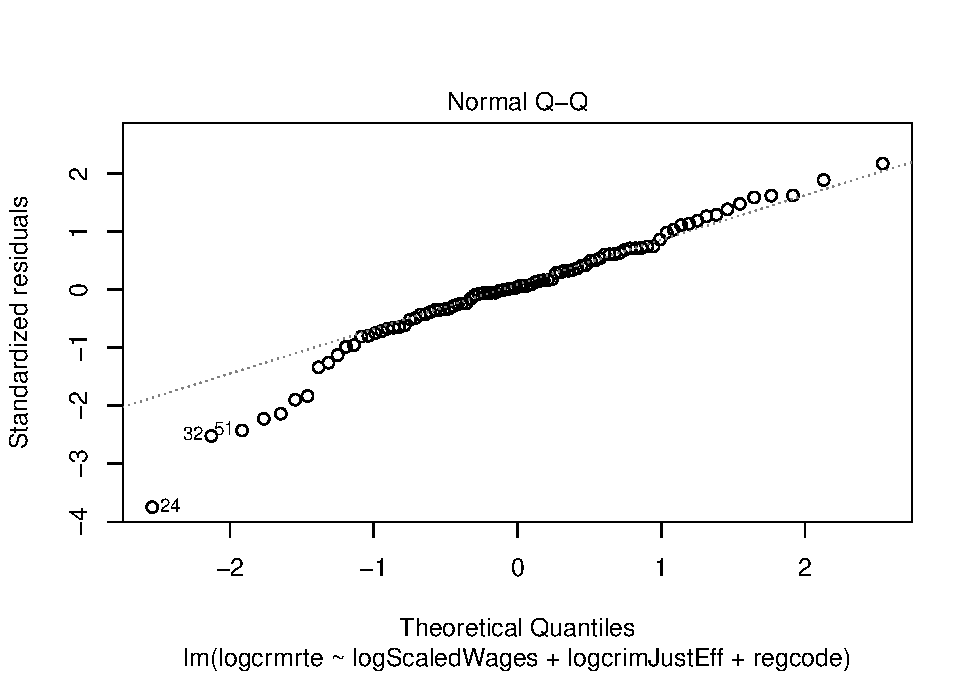
\includegraphics{Bagnard_Gaustad_Hartman_Leung_Lab_3_files/figure-latex/unnamed-chunk-65-1.pdf}

\hypertarget{model-1-interpretation}{%
\subsection{Model 1 Interpretation}\label{model-1-interpretation}}

The model 1 gives estimates and standard errors that are heteroskedastic
consistent. The coefficient of the log of unweighted average wage is
calculated to be \textasciitilde{}2. This means that an increase of 1\%
in wages is correlated with an increase of 2\% in crime rate. Generally
an individuals increased wages are not associated with increased crime.
This suggests that wages are correlated with a stronger omitted variable
that affects crime. One aspect that may be missed is the economic
inequality in the county. Averages are easily affected by extreme
values. It is possible that there are very high earners that can
influence a sector's average value, but don't represent the bulk of
workers. Further, there is no understanding of the weighting for each
sector. For example, one sector, like telecom, may have high wages in a
county but not have very many workers; further demonstrating inequality.
This detail is missed when each sector is rolled up into a single
average and then averaged with all other sector averages. However, the
significant result of wage on crime suggests that we are capturing some
cause of crime that is correlated to wages. We will continue to monitor
how wage changes as a predictor when introducing more regressors in
subsequent models.

Criminal justice effectiveness (convictions/crime) is given a
coefficient of \textasciitilde{}-0.5 which suggests that an increase of
1\% increase in convictions per crime will decrease crime by nearly
.5\%. This suggests that we have found a relatively strong correlation
and constructed a good operationalization of a county's criminal justice
effect on crime rate in a county. This variable will be monitored as we
add more regressors.

Region dummy variables of West and Central are both significant. This
suggests that regionally, there are differences that are not captured by
the Wages and Criminal Justice Effectiveness variable that affect crime.
While the West and Central regions both have lower crime than the
Coastal/Other region, the West is much more pronounced with a value of
\textasciitilde{}-0.6. This suggests that when correcting for
differences in Criminal Justice Effectiveness and Wages, the west will
still have crime rate lower by about 0.6\%.

Overall, the model shows a moderately good fit, with an adjusted R
square of 0.63. This can be interpreted as: the model explains 63\% of
the variation in crime. In the next model we will try to improve our
operationalization of economics and criminal justice by investigating
police per capita and tax revenue per capita.

\hypertarget{model-2}{%
\subsection{Model 2}\label{model-2}}

\hypertarget{introduction-2}{%
\subsubsection{Introduction}\label{introduction-2}}

In this model, we introduce the additional covariates of tax per capita
(taxpc) and police per capita (polpc) to increase the accuracy of our
regression. We are including these additional variables to our second
model, as they add accuracy to the explanatory variables used in our
first model:

--- why we are removing regcode as a direct variable

\begin{enumerate}
\def\labelenumi{\arabic{enumi}.}
\item
  The \textbf{Police Per Capita} in a county can be influential on the
  Criminal Justice Effectiveness. With more police in a given area, one
  would think that crime rates would decrease, however our correlation
  plot below tells a different story. Including this variable in our
  analysis will give us more insight into the variables used in model 1.
\item
  The \textbf{Tax Per Capita} can have a direct impact on the Police Per
  Capita. A higher tax per capita, means that the county has more tax
  dollars to spend on public services like the police force (ie.
  increasing the number of police in the county).
\end{enumerate}

\[logcrmrte = \beta_0 + \beta_1logScaledWages + \beta_2logcrimJustEff + \beta_3logpolpc * regcode + \beta_4logtaxpc + u\]

\hypertarget{model-2-eda-and-data-transformations}{%
\subsubsection{Model 2 EDA and Data
Transformations}\label{model-2-eda-and-data-transformations}}

Before we create our model, we will analyze each of the additional
variables to see if transformations are needed.

To start, we will look at the polpc variable:

\begin{Shaded}
\begin{Highlighting}[]
\NormalTok{p1 <-}\StringTok{ }\KeywordTok{ggplot}\NormalTok{(dfCrime, }\KeywordTok{aes}\NormalTok{(}\DataTypeTok{x =}\NormalTok{ polpc, }\DataTypeTok{color=}\NormalTok{regcode, }\DataTypeTok{fill =}\NormalTok{ regcode)) }\OperatorTok{+}\StringTok{ }
\StringTok{  }\KeywordTok{geom_histogram}\NormalTok{(}\DataTypeTok{position=}\StringTok{"identity"}\NormalTok{, }\DataTypeTok{alpha=}\FloatTok{0.5}\NormalTok{, }\DataTypeTok{bins=}\DecValTok{30}\NormalTok{) }\OperatorTok{+}
\StringTok{  }\KeywordTok{labs}\NormalTok{(}\DataTypeTok{title=}\StringTok{"Police per Capita"}\NormalTok{, }\DataTypeTok{x=}\StringTok{"Police per Capita"}\NormalTok{, }\DataTypeTok{y=}\StringTok{"Count"}\NormalTok{)}
\NormalTok{p2 <-}\StringTok{ }\KeywordTok{ggplot}\NormalTok{(dfCrime, }\KeywordTok{aes}\NormalTok{(}\DataTypeTok{x =} \KeywordTok{log}\NormalTok{(polpc), }\DataTypeTok{color=}\NormalTok{regcode, }\DataTypeTok{fill =}\NormalTok{ regcode)) }\OperatorTok{+}\StringTok{ }
\StringTok{  }\KeywordTok{geom_histogram}\NormalTok{(}\DataTypeTok{position=}\StringTok{"identity"}\NormalTok{, }\DataTypeTok{alpha=}\FloatTok{0.5}\NormalTok{, }\DataTypeTok{bins=}\DecValTok{30}\NormalTok{) }\OperatorTok{+}
\StringTok{  }\KeywordTok{labs}\NormalTok{(}\DataTypeTok{title=}\StringTok{"Log Transformed Police per Capita"}\NormalTok{, }\DataTypeTok{x=}\StringTok{"Log(Police per Capita)"}\NormalTok{, }\DataTypeTok{y=}\StringTok{"Count"}\NormalTok{)}
\KeywordTok{grid.arrange}\NormalTok{(p1, p2, }\DataTypeTok{ncol=}\DecValTok{2}\NormalTok{)}
\end{Highlighting}
\end{Shaded}

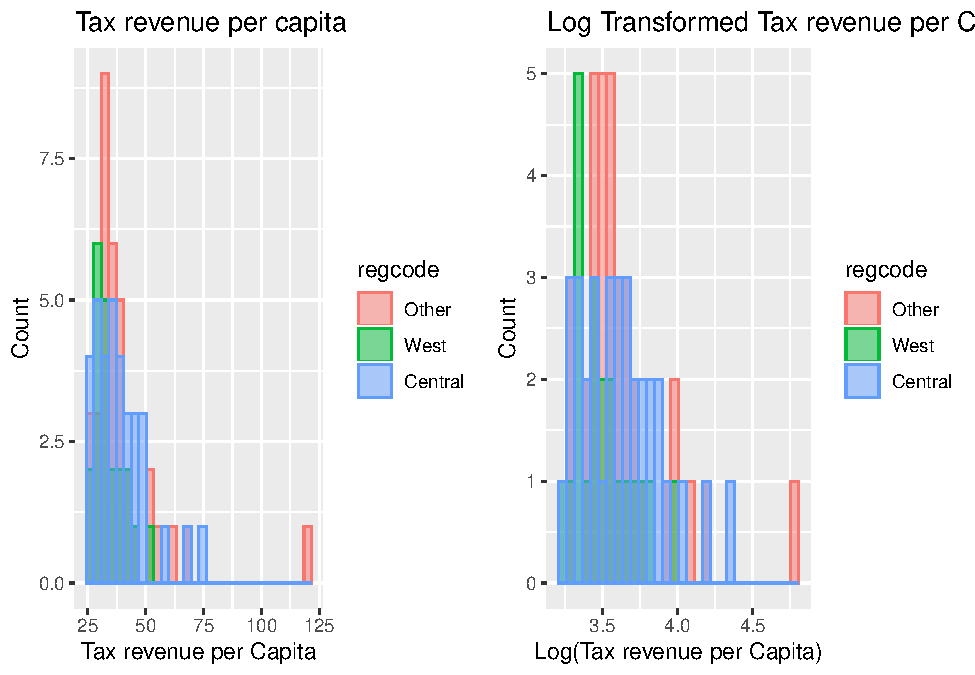
\includegraphics{Bagnard_Gaustad_Hartman_Leung_Lab_3_files/figure-latex/unnamed-chunk-66-1.pdf}

As we can see from the histograms above, taking the natural log of polpc
brings its distribution closer to normal. As a result, we will use the
log(polpc) in our analysis.

\begin{Shaded}
\begin{Highlighting}[]
\CommentTok{# creating the logpolpc variable}
\NormalTok{dfCrime}\OperatorTok{$}\NormalTok{logpolpc <-}\StringTok{ }\KeywordTok{log}\NormalTok{(dfCrime}\OperatorTok{$}\NormalTok{polpc)}
\end{Highlighting}
\end{Shaded}

Next, we will take a look at our taxpc variable to see if a
trasformation is warranted:

\begin{Shaded}
\begin{Highlighting}[]
\NormalTok{p1 <-}\StringTok{ }\KeywordTok{ggplot}\NormalTok{(dfCrime, }\KeywordTok{aes}\NormalTok{(}\DataTypeTok{x =}\NormalTok{ taxpc, }\DataTypeTok{color=}\NormalTok{regcode, }\DataTypeTok{fill =}\NormalTok{ regcode)) }\OperatorTok{+}\StringTok{ }
\StringTok{  }\KeywordTok{geom_histogram}\NormalTok{(}\DataTypeTok{position=}\StringTok{"identity"}\NormalTok{, }\DataTypeTok{alpha=}\FloatTok{0.5}\NormalTok{, }\DataTypeTok{bins=}\DecValTok{30}\NormalTok{) }\OperatorTok{+}
\StringTok{  }\KeywordTok{labs}\NormalTok{(}\DataTypeTok{title=}\StringTok{"Tax revenue per capita"}\NormalTok{, }\DataTypeTok{x=}\StringTok{"Tax revenue per Capita"}\NormalTok{, }\DataTypeTok{y=}\StringTok{"Count"}\NormalTok{)}
\NormalTok{p2 <-}\StringTok{ }\KeywordTok{ggplot}\NormalTok{(dfCrime, }\KeywordTok{aes}\NormalTok{(}\DataTypeTok{x =} \KeywordTok{log}\NormalTok{(taxpc), }\DataTypeTok{color=}\NormalTok{regcode, }\DataTypeTok{fill =}\NormalTok{ regcode)) }\OperatorTok{+}\StringTok{ }
\StringTok{  }\KeywordTok{geom_histogram}\NormalTok{(}\DataTypeTok{position=}\StringTok{"identity"}\NormalTok{, }\DataTypeTok{alpha=}\FloatTok{0.5}\NormalTok{, }\DataTypeTok{bins=}\DecValTok{30}\NormalTok{) }\OperatorTok{+}
\StringTok{  }\KeywordTok{labs}\NormalTok{(}\DataTypeTok{title=}\StringTok{"Log Transformed Tax revenue per Capita"}\NormalTok{, }\DataTypeTok{x=}\StringTok{"Log(Tax revenue per Capita)"}\NormalTok{, }\DataTypeTok{y=}\StringTok{"Count"}\NormalTok{)}
\KeywordTok{grid.arrange}\NormalTok{(p1, p2, }\DataTypeTok{ncol=}\DecValTok{2}\NormalTok{)}
\end{Highlighting}
\end{Shaded}

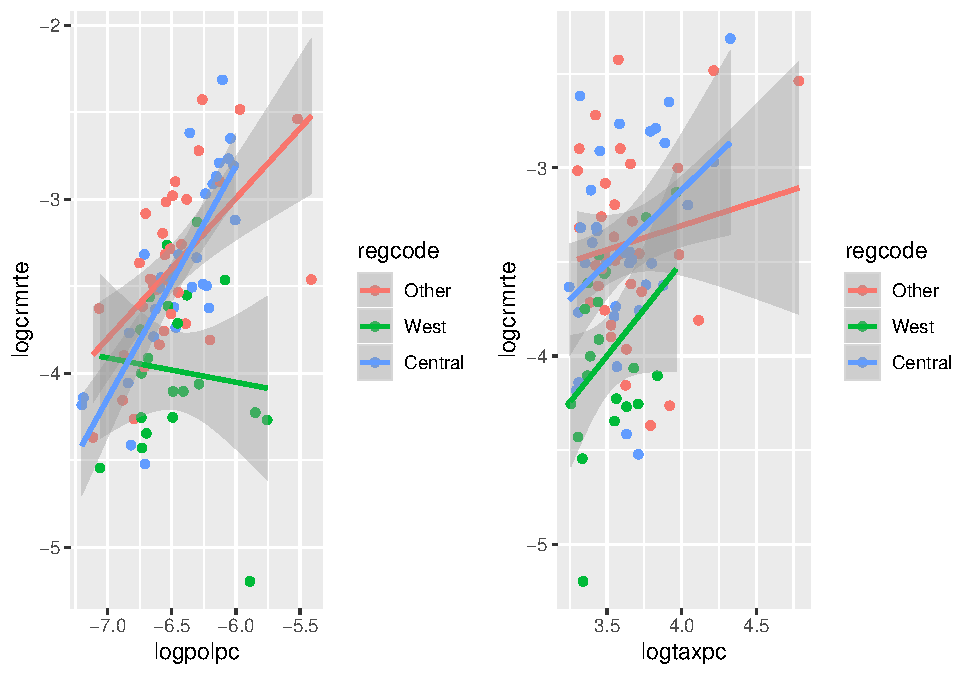
\includegraphics{Bagnard_Gaustad_Hartman_Leung_Lab_3_files/figure-latex/unnamed-chunk-68-1.pdf}
The histogram of taxpc, depicts each region as having an approximately
normal distribution with each cenetred on a different mean. When we take
the natural log of taxpc, we can see in the histogram, above, that each
region has a more normal distribution. In addition, taking the natural
log of taxpc reduces the extremity of the outlier seen in histogram of
taxpc. As a result, we will use the log(taxpc) in our analysis.

\begin{Shaded}
\begin{Highlighting}[]
\NormalTok{dfCrime}\OperatorTok{$}\NormalTok{logtaxpc <-}\StringTok{ }\KeywordTok{log}\NormalTok{(dfCrime}\OperatorTok{$}\NormalTok{taxpc)}
\end{Highlighting}
\end{Shaded}

Now that we have transformed the two variables we are adding to model
two, we will take a look at how logtaxpc and logpolpc relate to
logcrmrate and if these trends vary between each regcode.

-- SHOULD WE MENTION WHY WE ARE LOOKING AT THIS BY REGCODE --

\begin{Shaded}
\begin{Highlighting}[]
\NormalTok{logpolpc_plot<-}\KeywordTok{ggplot}\NormalTok{(}\DataTypeTok{data =}\NormalTok{ dfCrime, }\KeywordTok{aes}\NormalTok{(}\DataTypeTok{x =}\NormalTok{ logpolpc, }\DataTypeTok{y =}\NormalTok{ logcrmrte, }\DataTypeTok{color =}\NormalTok{ regcode)) }\OperatorTok{+}\StringTok{ }
\StringTok{      }\KeywordTok{geom_point}\NormalTok{()}\OperatorTok{+}
\StringTok{  }\KeywordTok{geom_smooth}\NormalTok{(}\DataTypeTok{method =} \StringTok{"lm"}\NormalTok{)}
\NormalTok{logtaxpc_plot<-}\KeywordTok{ggplot}\NormalTok{(}\DataTypeTok{data =}\NormalTok{ dfCrime, }\KeywordTok{aes}\NormalTok{(}\DataTypeTok{x =}\NormalTok{ logtaxpc, }\DataTypeTok{y =}\NormalTok{ logcrmrte, }\DataTypeTok{color =}\NormalTok{ regcode)) }\OperatorTok{+}\StringTok{ }
\StringTok{      }\KeywordTok{geom_point}\NormalTok{()}\OperatorTok{+}
\StringTok{  }\KeywordTok{geom_smooth}\NormalTok{(}\DataTypeTok{method =} \StringTok{"lm"}\NormalTok{)}

\KeywordTok{options}\NormalTok{(}\DataTypeTok{repr.plot.width=}\DecValTok{8}\NormalTok{, }\DataTypeTok{repr.plot.height=}\DecValTok{16}\NormalTok{)}
\KeywordTok{grid.arrange}\NormalTok{(logpolpc_plot,logtaxpc_plot, }\DataTypeTok{ncol=}\DecValTok{2}\NormalTok{)}
\end{Highlighting}
\end{Shaded}

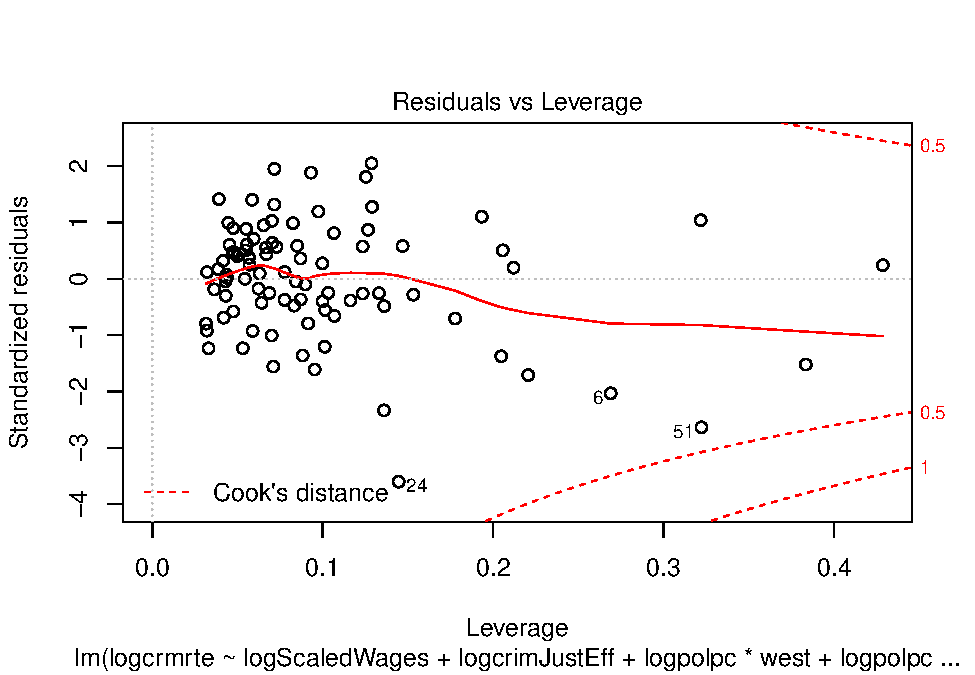
\includegraphics{Bagnard_Gaustad_Hartman_Leung_Lab_3_files/figure-latex/unnamed-chunk-70-1.pdf}

Right away, we can see clear difference between each regions' logpolpc
regression on logcrmerte.``Other'' and ``Central'' regions have
positively slopped regression lines, while ``West'' has a negatively
slopped regression line. This suggests that we should investigate the
interactions between logpolpc and region (regcode) in our model.

logtaxpc to logcrmrte, on the other hand, does not demonstrate this
regression slope variation between each regions. As result, we will not
look into the interactions between logtaxpc and region in our model.

-- DELETE -- NOTES: -regionally we see a difference in the polpc
regression on crime rate - this suggests that we should investigate the
interaction between polpc and region. --\textgreater{} law enforcement
style could be different in the regions which.\\
- we do not need to look at taxpc and region as the slopes do not vary
greatly across regions. -----

\hypertarget{model-2-linear-model}{%
\subsubsection{Model 2 Linear Model}\label{model-2-linear-model}}

\[logcrmrte = \beta_0 + \beta_1logScaledWages + \beta_2logcrimJustEff + \beta_3logpolpc * regcode + \beta_4logtaxpc + u\]

\begin{Shaded}
\begin{Highlighting}[]
\NormalTok{model2 <-}\StringTok{ }\KeywordTok{lm}\NormalTok{(logcrmrte }\OperatorTok{~}\StringTok{ }\NormalTok{logScaledWages }\OperatorTok{+}\StringTok{ }\NormalTok{logcrimJustEff }\OperatorTok{+}\StringTok{ }\NormalTok{logpolpc}\OperatorTok{*}\NormalTok{regcode }\OperatorTok{+}\StringTok{ }\NormalTok{logtaxpc, }\DataTypeTok{data =}\NormalTok{ dfCrime)}
\NormalTok{model2}
\end{Highlighting}
\end{Shaded}

\begin{verbatim}

Call:
lm(formula = logcrmrte ~ logScaledWages + logcrimJustEff + logpolpc * 
    regcode + logtaxpc, data = dfCrime)

Coefficients:
            (Intercept)           logScaledWages           logcrimJustEff  
                -6.9290                   1.1983                  -0.4233  
               logpolpc              regcodeWest           regcodeCentral  
                 0.5627                  -5.8101                   0.9987  
               logtaxpc     logpolpc:regcodeWest  logpolpc:regcodeCentral  
                -0.1537                  -0.8029                   0.1853  
\end{verbatim}

\begin{Shaded}
\begin{Highlighting}[]
\KeywordTok{summary}\NormalTok{(model2)}\OperatorTok{$}\NormalTok{adj.r.square}
\end{Highlighting}
\end{Shaded}

\begin{verbatim}
[1] 0.7016715
\end{verbatim}

From the Residuals vs Leverage graph, below, we can see that our model
does not contain any outliers with have significant influence (ie. there
are no points with a Cook's distance of 0.5 or greater).

\begin{Shaded}
\begin{Highlighting}[]
\KeywordTok{plot}\NormalTok{(model2, }\DataTypeTok{which=}\DecValTok{5}\NormalTok{) }
\end{Highlighting}
\end{Shaded}

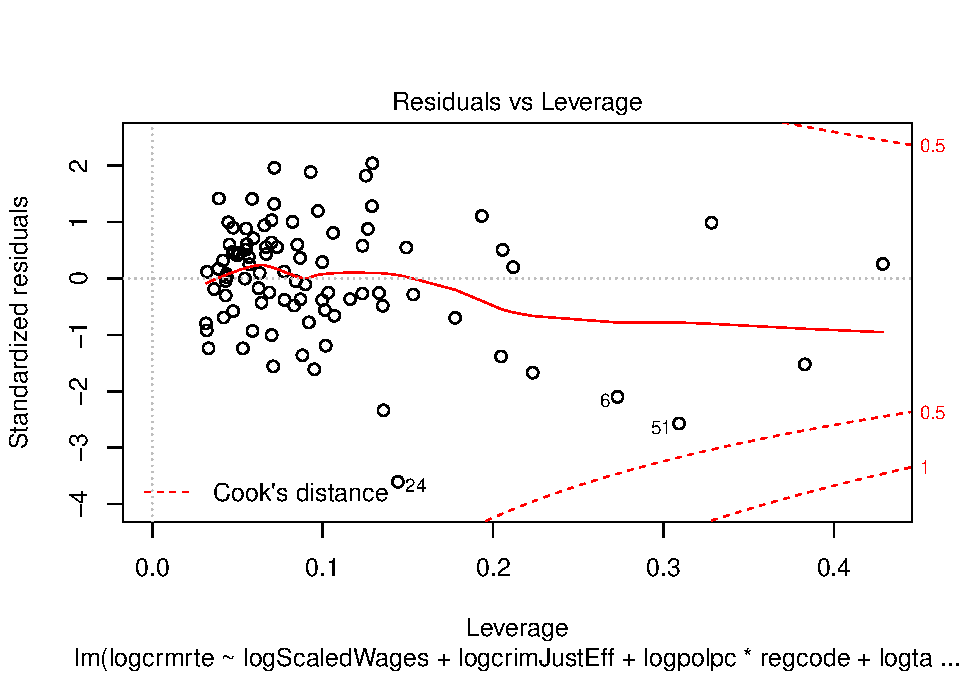
\includegraphics{Bagnard_Gaustad_Hartman_Leung_Lab_3_files/figure-latex/unnamed-chunk-72-1.pdf}

\textbf{Model 2 CLM Assumptions:}

\begin{itemize}
\item
  \textbf{MLR1} Discussed above.
\item
  \textbf{MLR2} Discussed above.
\item
  \textbf{MLR3: Non-perfect Collinearity} We will use the VIF function
  to provide evidence that our variables in model2 are not perfectly
  multicollinear. As we can see from the VIF results, below, all of the
  variables' values are less than five, which allows us to conclude
  model2 is free from multicollinearity.
\end{itemize}

\begin{Shaded}
\begin{Highlighting}[]
\KeywordTok{vif}\NormalTok{(model2)}
\end{Highlighting}
\end{Shaded}

\begin{verbatim}
##                          GVIF Df GVIF^(1/(2*Df))
## logScaledWages   1.581951e+00  1        1.257756
## logcrimJustEff   1.204326e+00  1        1.097418
## logpolpc         3.186691e+00  1        1.785130
## regcode          1.921406e+05  2       20.936535
## logtaxpc         1.435072e+00  1        1.197945
## logpolpc:regcode 1.893355e+05  2       20.859699
\end{verbatim}

\begin{itemize}
\tightlist
\item
  \textbf{MLR4: Zero Conditional Mean} The residual vs.~fitted chart,
  below, gives us evidence that we meet the zero conditional mean
  assumption as the majority of the residual means lie close to zero.
  The exceptions to this trend, lie on the left and right sides of the
  chart where there are fewer data points (evidence for
  heteroscedasticity - see MLR5, below).
\end{itemize}

\begin{Shaded}
\begin{Highlighting}[]
\KeywordTok{plot}\NormalTok{(model2, }\DataTypeTok{which=}\DecValTok{1}\NormalTok{)}
\end{Highlighting}
\end{Shaded}

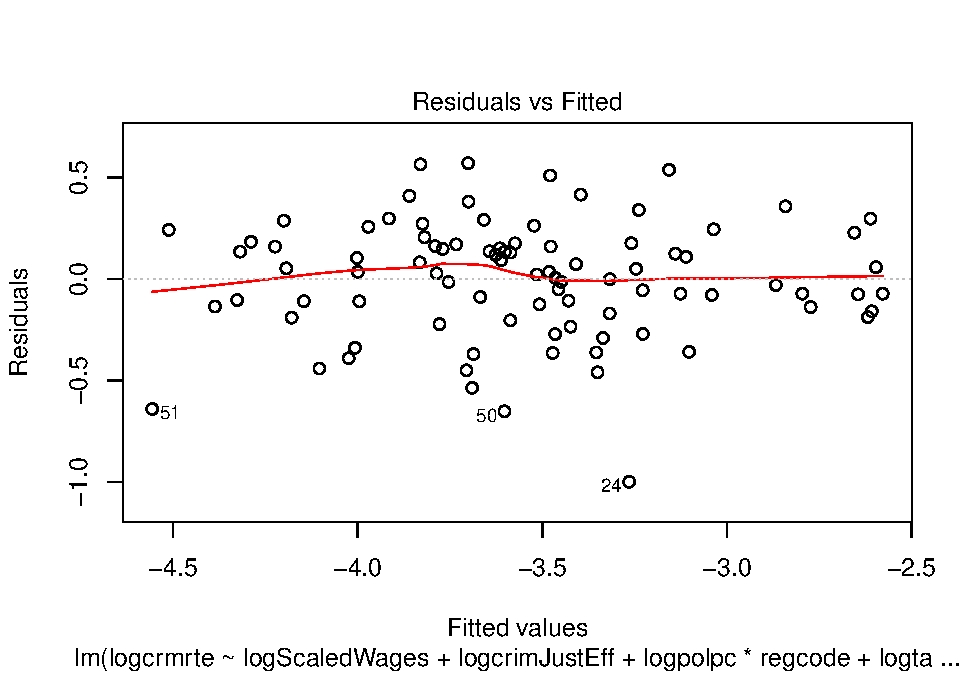
\includegraphics{Bagnard_Gaustad_Hartman_Leung_Lab_3_files/figure-latex/unnamed-chunk-74-1.pdf}

\begin{itemize}
\tightlist
\item
  \textbf{MLR5: Homoscedasticity} The above Residuals vs Fitted graph
  provides evidence of heteroscedasticity as right side of the chart
  have fewer datepoints. To provide further evidence of
  heteroscedasticity, we will use the White-Huber test with the vcovHC
  method to generate coefficients that are robust to heteroscedasticity
\end{itemize}

\begin{Shaded}
\begin{Highlighting}[]
\KeywordTok{coeftest}\NormalTok{(model2, }\DataTypeTok{vcov=}\NormalTok{vcovHC)}
\end{Highlighting}
\end{Shaded}

\begin{verbatim}

t test of coefficients:

                        Estimate Std. Error t value  Pr(>|t|)    
(Intercept)             -6.92901    3.59156 -1.9292 0.0572019 .  
logScaledWages           1.19829    0.47104  2.5439 0.0128622 *  
logcrimJustEff          -0.42334    0.10629 -3.9829 0.0001479 ***
logpolpc                 0.56271    0.25285  2.2255 0.0288270 *  
regcodeWest             -5.81007    2.91439 -1.9936 0.0495635 *  
regcodeCentral           0.99869    1.43754  0.6947 0.4892159    
logtaxpc                -0.15372    0.18966 -0.8105 0.4200320    
logpolpc:regcodeWest    -0.80290    0.44556 -1.8020 0.0752643 .  
logpolpc:regcodeCentral  0.18529    0.22006  0.8420 0.4022610    
---
Signif. codes:  0 '***' 0.001 '**' 0.01 '*' 0.05 '.' 0.1 ' ' 1
\end{verbatim}

As we can see from the coeftest results above, the interactions between
logpolpc and regcode west and central are not statistically significant
(at least by themselves).

However, they may be jointly significant. We will run a f-test to see if
this might be the case:

\begin{Shaded}
\begin{Highlighting}[]
\KeywordTok{linearHypothesis}\NormalTok{(model2, }\KeywordTok{c}\NormalTok{(}\StringTok{"logpolpc:regcodeWest=0"}\NormalTok{, }\StringTok{"logpolpc:regcodeCentral"}\NormalTok{), }\DataTypeTok{vcov=}\NormalTok{vcovHC)}
\end{Highlighting}
\end{Shaded}

\begin{verbatim}
## Linear hypothesis test
## 
## Hypothesis:
## logpolpc:regcodeWest = 0
## logpolpc:regcodeCentral = 0
## 
## Model 1: restricted model
## Model 2: logcrmrte ~ logScaledWages + logcrimJustEff + logpolpc * regcode + 
##     logtaxpc
## 
## Note: Coefficient covariance matrix supplied.
## 
##   Res.Df Df      F Pr(>F)  
## 1     83                   
## 2     81  2 3.0147 0.0546 .
## ---
## Signif. codes:  0 '***' 0.001 '**' 0.01 '*' 0.05 '.' 0.1 ' ' 1
\end{verbatim}

We can see frome the f-test, above, that the interactions between
logpolpc and regcodes west and central are not statistically significant
to the model.

-- DELETE --- NOTES: INTERACTIONS BETWETEEN POLPC AND REGCODE WEST AND
CENTRAL ARE NOT BY THEMSELVES SIGNIFICANT. LETS F TEST TO SEE IF THEY
ARE JOINTLY SIGNIFICANT\ldots{}and they are barely not significant. The
dummy variable for central is not significant which suggests that
central and other are very similar while west is different. ---

\begin{itemize}
\tightlist
\item
  \textbf{MLR6: Normal Distribution of Errors} The Normal Q-Q plot,
  below, provides evidence that our residuals follow a normal
  distribution. While there are some data points on the left and right
  side of the graph that stray from the diagonal line, since our data
  set has over 30 datapoints, per the CLT, we can assume residuals have
  a normal distribution.
\end{itemize}

\begin{Shaded}
\begin{Highlighting}[]
\KeywordTok{plot}\NormalTok{(model2, }\DataTypeTok{which=}\DecValTok{2}\NormalTok{)}
\end{Highlighting}
\end{Shaded}

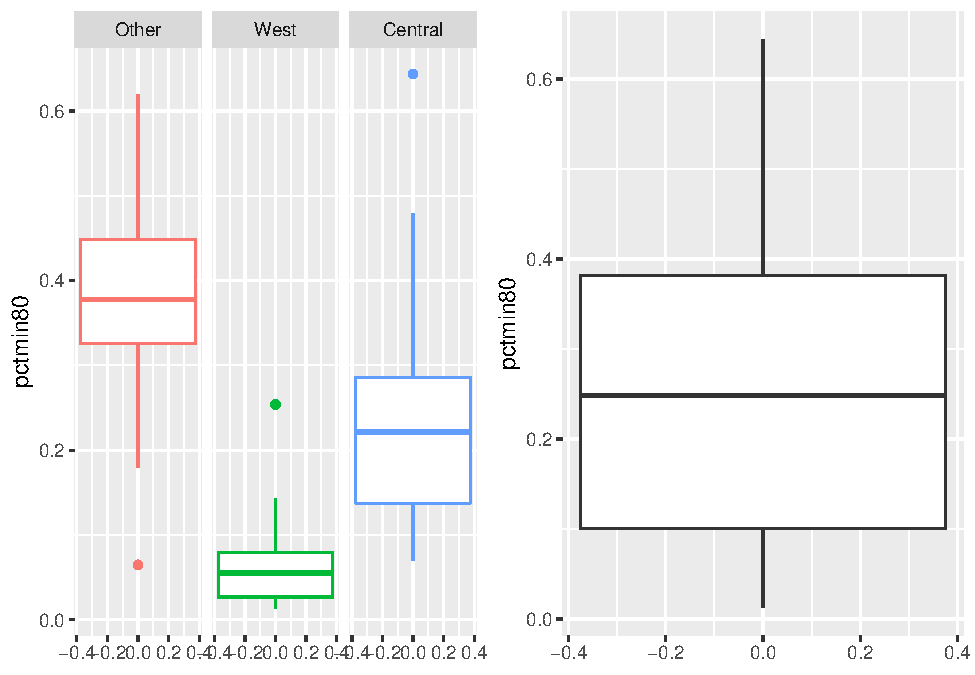
\includegraphics{Bagnard_Gaustad_Hartman_Leung_Lab_3_files/figure-latex/unnamed-chunk-77-1.pdf}

\begin{Shaded}
\begin{Highlighting}[]
\CommentTok{# hist(model2$residuals)}
\CommentTok{#shapiro.test(model2$residuals)}
\CommentTok{#null hypothesis: residuals drawn from population with a normal distribution. }
\CommentTok{#small p-value tells you if you can reject the null hypothesis. }
\CommentTok{#this test depends on sample size, it does not take very much deviation from normality for}
\CommentTok{#us to get a statistically significant result}
\end{Highlighting}
\end{Shaded}

\begin{Shaded}
\begin{Highlighting}[]
\KeywordTok{summary}\NormalTok{(model2)}
\end{Highlighting}
\end{Shaded}

\begin{verbatim}
## 
## Call:
## lm(formula = logcrmrte ~ logScaledWages + logcrimJustEff + logpolpc * 
##     regcode + logtaxpc, data = dfCrime)
## 
## Residuals:
##     Min      1Q  Median      3Q     Max 
## -0.9994 -0.1536  0.0318  0.1749  0.5711 
## 
## Coefficients:
##                         Estimate Std. Error t value Pr(>|t|)    
## (Intercept)             -6.92901    2.82987  -2.449  0.01650 *  
## logScaledWages           1.19829    0.37049   3.234  0.00177 ** 
## logcrimJustEff          -0.42334    0.06035  -7.015  6.3e-10 ***
## logpolpc                 0.56271    0.17235   3.265  0.00161 ** 
## regcodeWest             -5.81007    1.72493  -3.368  0.00116 ** 
## regcodeCentral           0.99869    1.47399   0.678  0.49999    
## logtaxpc                -0.15372    0.14361  -1.070  0.28763    
## logpolpc:regcodeWest    -0.80290    0.26596  -3.019  0.00339 ** 
## logpolpc:regcodeCentral  0.18529    0.22707   0.816  0.41688    
## ---
## Signif. codes:  0 '***' 0.001 '**' 0.01 '*' 0.05 '.' 0.1 ' ' 1
## 
## Residual standard error: 0.2997 on 81 degrees of freedom
## Multiple R-squared:  0.7285, Adjusted R-squared:  0.7017 
## F-statistic: 27.17 on 8 and 81 DF,  p-value: < 2.2e-16
\end{verbatim}

The Adjusted R-squared variable penalizes for additional variables,
which means there is a chance that this value will decrease if the added
variables do not contribute to the model. By comparing the Adjusted
R-squared value between our first and second models, we see that
logtaxpc and the interaction between logpolpc and regcode help describe
logcrmrte.

Our second model has an Adjusted R-squared value of 0.6989, which means
69.89\% of the variation in the natural log of the crime rate is
explained by the explanatory variables used in this model. This is a
slight increase compared to our first model, that has an Adjusted
R-squared value of 0.6345.

In addition, the F-statistic is 26.83 with a statistically significant
p-value of \textless{} 2.2e-16. As a result, we reject the null
hypothesis that none of the independent variables help to describe
logcrmrte.

Coefficient Analysis (assuming ceterus paribus): - logcrimJustEff:
-0.1607. This suggests that for a 1\% increase in criminal justice
efficiency, there is a 0.1607\% decrease in crime rate. - logpolpc:
0.3701. This suggests that for a 1\% increase in police per capita,
there is a 0.3701\% increase in crime rate. - scaledWages: 0.00006692.
This suggests that for a 1\% increase in total average weekly wage,
there is a 0.0067\% increase in crime rate. - taxpc: -0.001632. This
suggests that for a 1\% increase in tax per capita, there is a 0.1632\%
decrease in crime rate. - density: 0.06259. This suggests that for a 1\%
increase in density, there is a 6.259\% increase in crime rate.

\hypertarget{conclusion-are-the-conclusions-they-draw-based-on-this-evaluation-appropriate-did-the-team-interpret-the-results-in-terms-of-their-research-question}{%
\subsubsection{Conclusion : Are the conclusions they draw based on this
evaluation appropriate? Did the team interpret the results in terms of
their research
question?}\label{conclusion-are-the-conclusions-they-draw-based-on-this-evaluation-appropriate-did-the-team-interpret-the-results-in-terms-of-their-research-question}}

Compared to model 1, the adjusted \(R^2\) of model 2 is only marginally
higher. This suggests that we should continue our analysis by focusing
on the join significance of the variables added in model 2.

\hypertarget{model-3}{%
\subsection{Model 3}\label{model-3}}

\hypertarget{discussion-of-variables}{%
\subsubsection{Discussion of Variables}\label{discussion-of-variables}}

From Model 2, we noted that the addition of the transformed variable
logpolpc had statistical significance and helped improve the fit of the
model, as measured by adjusted R-squared, to 70\%. To increase our
understanding at the linkages between police presence, economic
conditions, criminal justice effectiveness and region, we propose to
also analyse the areas of demographics which could have an effect on
both of our key explanatory variables.

\textbf{Minorities} One key component of demographics is the race of the
county inhabitants and how they are perceived and treated by others,
especially for minorities in the population. For example, systemic
racism could have an important effect on: * Criminal Justice
Effectiveness: If police, lawyers and judges are racially biased, this
could lead to more arrests and more convictions regardless of the
strength of the legal case and the evidence. As a result, we hypothesize
the crime rate would increase. * Economic Opportunity: Racism could
prohibit members of the minority from having access to education, jobs
and higher wages. Racism could also limit access to healthcare and
social programmes which has a negative effect on economic opportunity.

However, since we cannot directly measure racism, we have to
operationalize this covariate by examining its effect in the real world.
We propose to use the variable pctmin80, which represents the percentage
of minorities in the population of the county. This is also a continous
parameter and so given a higher the percentage of minorities, we should
expect to see a greater effect.

From the summary and boxplot below, we can see that the percentage of
minorities ranges from 0.0154 - 0.6435, with a mean of 0.2621. We note
that there are no major outliers. In addition, different regions and
counties can have different demographics. We can see from the boxplots
below that counties in the West have a significantly lower percentage of
minorities than the other two regions.

We will apply the natural log to the variable pctmin80 to 1) make it
easier for us to interpret the coefficient in our linear model and 2) to
better expose the linear relationship in the model.

\begin{Shaded}
\begin{Highlighting}[]
\KeywordTok{summary}\NormalTok{(dfCrime}\OperatorTok{$}\NormalTok{pctmin80)}
\end{Highlighting}
\end{Shaded}

\begin{verbatim}
   Min. 1st Qu.  Median    Mean 3rd Qu.    Max. 
0.01284 0.10024 0.24852 0.25713 0.38183 0.64348 
\end{verbatim}

\begin{Shaded}
\begin{Highlighting}[]
\KeywordTok{options}\NormalTok{(}\DataTypeTok{repr.plot.width=}\DecValTok{8}\NormalTok{, }\DataTypeTok{repr.plot.height=}\DecValTok{4}\NormalTok{)}
\NormalTok{p<-}\KeywordTok{ggplot}\NormalTok{(}\DataTypeTok{data =}\NormalTok{ dfCrime, }\KeywordTok{aes}\NormalTok{(}\DataTypeTok{y =}\NormalTok{ pctmin80, }\DataTypeTok{color =}\NormalTok{ regcode)) }\OperatorTok{+}\StringTok{ }
\StringTok{     }\KeywordTok{geom_boxplot}\NormalTok{(}\DataTypeTok{show.legend=}\OtherTok{FALSE}\NormalTok{) }\OperatorTok{+}\StringTok{ }\KeywordTok{facet_wrap}\NormalTok{(}\OperatorTok{~}\StringTok{ }\NormalTok{regcode)}
\NormalTok{p2<-}\KeywordTok{ggplot}\NormalTok{(}\DataTypeTok{data =}\NormalTok{ dfCrime, }\KeywordTok{aes}\NormalTok{(}\DataTypeTok{y =}\NormalTok{ pctmin80)) }\OperatorTok{+}
\StringTok{     }\KeywordTok{geom_boxplot}\NormalTok{()}
\KeywordTok{grid.arrange}\NormalTok{(p, p2, }\DataTypeTok{ncol=}\DecValTok{2}\NormalTok{)}
\end{Highlighting}
\end{Shaded}

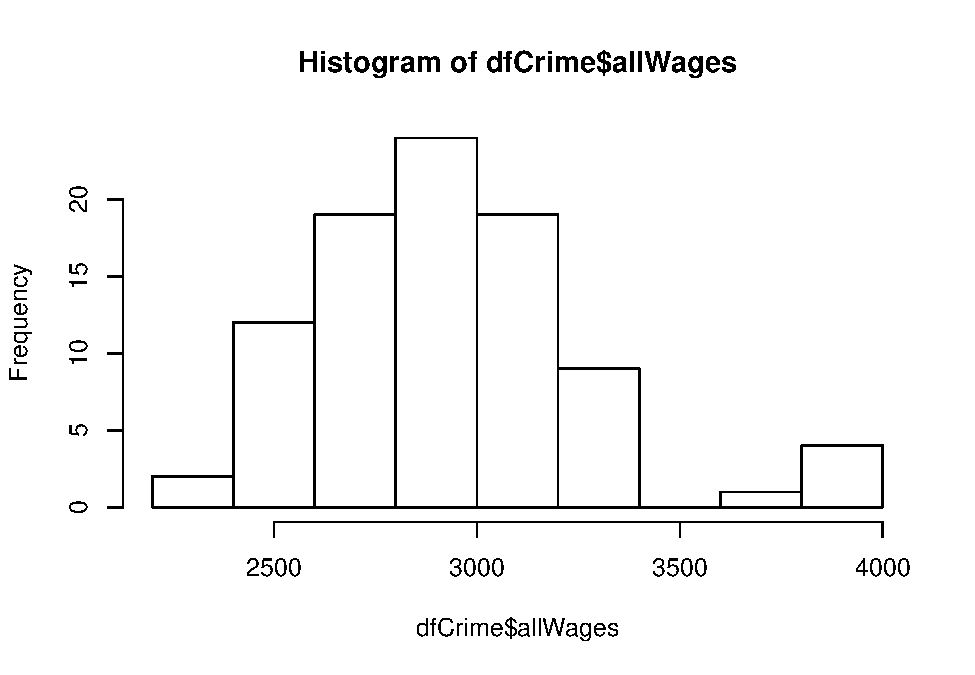
\includegraphics{Bagnard_Gaustad_Hartman_Leung_Lab_3_files/figure-latex/unnamed-chunk-79-1.pdf}

\begin{Shaded}
\begin{Highlighting}[]
\NormalTok{dfCrime}\OperatorTok{$}\NormalTok{logpctmin80 <-}\StringTok{ }\KeywordTok{log}\NormalTok{(dfCrime}\OperatorTok{$}\NormalTok{pctmin80)}
\end{Highlighting}
\end{Shaded}

\textbf{Density} Another component of demographics is the population
density, which can have impacts that may be positive or negative on the
crime rate: - \textbf{Criminal Justice Effectiveness}: With more people
in a given area, there may be more opportunities for more people to
commit crimes. However, a higher density may also result in higher
deterents such as more eyewitnesses or faster law-enforcement response
rates. - \textbf{Economic Opportunity (ie. scaledWages)}: In high
density areas, there is an increase in demand for support services such
as food, retail, utilities, etc. As a result, there is a high demand for
service jobs, which increases the economic opportunities within the
area. However, more people in a given area, there is a closer proximity
to drugs, alcohol and gang violence - all of which are inhibitors to
better economic outcomes.

From the summary and boxplot below, we can see that the density ranges
from 0.3006 - 8.8277, with a mean of 0.9792 persons per square mile. We
note that while there are some outliers to the data, this does not
appear at first glance to be an issue as some counties can contain major
cities which would naturally lead to a higher population density. As a
result, we will not make adjustments to any outliers unless we detect
datapoints having high influence in our model.

\begin{Shaded}
\begin{Highlighting}[]
\KeywordTok{summary}\NormalTok{(dfCrime}\OperatorTok{$}\NormalTok{density)}
\end{Highlighting}
\end{Shaded}

\begin{verbatim}
##    Min. 1st Qu.  Median    Mean 3rd Qu.    Max. 
##  0.3006  0.5506  0.9792  1.4419  1.5693  8.8277
\end{verbatim}

\begin{Shaded}
\begin{Highlighting}[]
\KeywordTok{options}\NormalTok{(}\DataTypeTok{repr.plot.width=}\DecValTok{8}\NormalTok{, }\DataTypeTok{repr.plot.height=}\DecValTok{4}\NormalTok{)}
\NormalTok{p<-}\KeywordTok{ggplot}\NormalTok{(}\DataTypeTok{data =}\NormalTok{ dfCrime, }\KeywordTok{aes}\NormalTok{(}\DataTypeTok{y =}\NormalTok{ density, }\DataTypeTok{color =}\NormalTok{ regcode)) }\OperatorTok{+}\StringTok{ }
\StringTok{     }\KeywordTok{geom_boxplot}\NormalTok{(}\DataTypeTok{show.legend=}\OtherTok{FALSE}\NormalTok{) }\OperatorTok{+}\StringTok{ }\KeywordTok{facet_wrap}\NormalTok{(}\OperatorTok{~}\StringTok{ }\NormalTok{regcode)}
\NormalTok{p2<-}\KeywordTok{ggplot}\NormalTok{(}\DataTypeTok{data =}\NormalTok{ dfCrime, }\KeywordTok{aes}\NormalTok{(}\DataTypeTok{y =}\NormalTok{ density)) }\OperatorTok{+}
\StringTok{     }\KeywordTok{geom_boxplot}\NormalTok{()}
\KeywordTok{grid.arrange}\NormalTok{(p, p2, }\DataTypeTok{ncol=}\DecValTok{2}\NormalTok{)}
\end{Highlighting}
\end{Shaded}

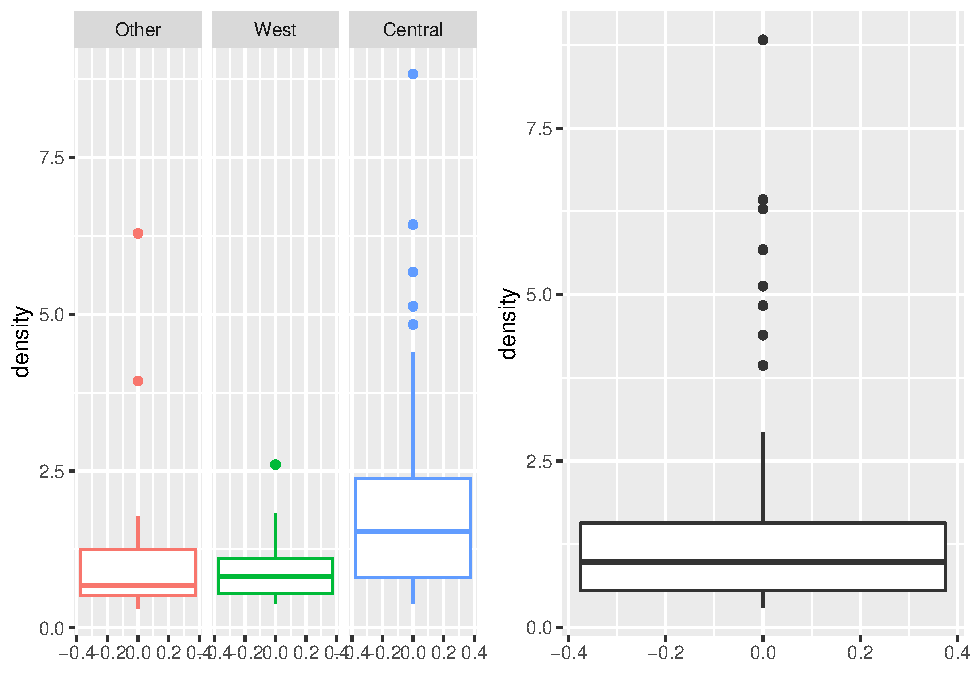
\includegraphics{Bagnard_Gaustad_Hartman_Leung_Lab_3_files/figure-latex/unnamed-chunk-80-1.pdf}

\textbf{Variables not considered} We have also chosen not to include
other variables from our dataset in our model: * Urban: We believe the
variable ``density'' better explains the same effects as ``urban'' while
also being a continous. We believe a continous variable is more
meaningful rather a binary indicator such as urban as there may be data
points that failed to meet the cutoff for being defined as urban, but
may still see the same effects as being urban and hence may distort our
analysis. * Age and Gender: While age and gender are important
demographic variables, the only variable in our dataset is pctymle which
provides the percentage of young males in the population. However, given
that this variable encompasses both male and young, we may not be able
to discern if age or gender has the larger effect (if any at all). *
Judgement: We chose not to include the varibles concerning the
probability of a prison sentence as well as the average sentence as we
believe it is unlikely that potential criminals would have good access
to this information. In addition, local county officials have limited
influence over the decisions of the judiciary system, as they are
separate branches of government.

Our equation for model 3 is as follows:
\[log(crmrate) = \beta_0 + \beta_1log(scaledWages) + \beta_2log(crimjusteff) + \beta_3regcode + \beta_4log(polpc) + \beta_5log(taxpc)+ \beta_6log(pctmin80) + \beta_7density +u\]

\hypertarget{model-3-linear-model}{%
\subsubsection{Model 3 Linear Model}\label{model-3-linear-model}}

\begin{Shaded}
\begin{Highlighting}[]
\NormalTok{model3_initial<-}\KeywordTok{lm}\NormalTok{(logcrmrte }\OperatorTok{~}\StringTok{ }\NormalTok{logScaledWages }\OperatorTok{+}\StringTok{ }\NormalTok{logcrimJustEff   }\OperatorTok{+}\StringTok{  }\NormalTok{regcode }\OperatorTok{+}\StringTok{ }\NormalTok{logpolpc }\OperatorTok{+}\StringTok{ }\NormalTok{logtaxpc }\OperatorTok{+}\StringTok{ }\NormalTok{logpctmin80 }\OperatorTok{+}\StringTok{ }\NormalTok{density, }\DataTypeTok{data =}\NormalTok{ dfCrime)}
\KeywordTok{summary}\NormalTok{(model3_initial)}
\end{Highlighting}
\end{Shaded}

\begin{verbatim}

Call:
lm(formula = logcrmrte ~ logScaledWages + logcrimJustEff + regcode + 
    logpolpc + logtaxpc + logpctmin80 + density, data = dfCrime)

Residuals:
     Min       1Q   Median       3Q      Max 
-0.89661 -0.14182  0.04774  0.12927  0.67395 

Coefficients:
               Estimate Std. Error t value Pr(>|t|)    
(Intercept)    -7.74182    2.59592  -2.982  0.00378 ** 
logScaledWages  1.07484    0.38552   2.788  0.00661 ** 
logcrimJustEff -0.41430    0.06193  -6.690 2.66e-09 ***
regcodeWest    -0.21857    0.13489  -1.620  0.10906    
regcodeCentral -0.16269    0.07999  -2.034  0.04525 *  
logpolpc        0.31614    0.11462   2.758  0.00718 ** 
logtaxpc       -0.14307    0.13531  -1.057  0.29351    
logpctmin80     0.19156    0.05428   3.529  0.00069 ***
density         0.08797    0.02952   2.980  0.00380 ** 
---
Signif. codes:  0 '***' 0.001 '**' 0.01 '*' 0.05 '.' 0.1 ' ' 1

Residual standard error: 0.2829 on 81 degrees of freedom
Multiple R-squared:  0.758, Adjusted R-squared:  0.7341 
F-statistic: 31.72 on 8 and 81 DF,  p-value: < 2.2e-16
\end{verbatim}

We note from the the summary above and the F-tests below that west and
central were not statistically significant to the model, but the
inclusion of logpctmin80 and density are significant at the 99\%
confidence level. It appears that our new variables better explain the
variation between counties rather than purely based on their geographic
location and we thus remove the latter 2 variables from our model.

\begin{Shaded}
\begin{Highlighting}[]
\KeywordTok{linearHypothesis}\NormalTok{(model3_initial,}\KeywordTok{c}\NormalTok{(}\StringTok{"regcodeWest=0"}\NormalTok{,}\StringTok{"regcodeCentral=0"}\NormalTok{), }\DataTypeTok{vcov=}\NormalTok{vcovHC)}
\end{Highlighting}
\end{Shaded}

\begin{verbatim}
## Linear hypothesis test
## 
## Hypothesis:
## regcodeWest = 0
## regcodeCentral = 0
## 
## Model 1: restricted model
## Model 2: logcrmrte ~ logScaledWages + logcrimJustEff + regcode + logpolpc + 
##     logtaxpc + logpctmin80 + density
## 
## Note: Coefficient covariance matrix supplied.
## 
##   Res.Df Df      F Pr(>F)
## 1     83                 
## 2     81  2 1.5194  0.225
\end{verbatim}

\begin{Shaded}
\begin{Highlighting}[]
\KeywordTok{vif}\NormalTok{(model3_initial)}
\end{Highlighting}
\end{Shaded}

\begin{verbatim}
##                    GVIF Df GVIF^(1/(2*Df))
## logScaledWages 1.922007  1        1.386365
## logcrimJustEff 1.423236  1        1.192995
## regcode        3.709750  2        1.387830
## logpolpc       1.581567  1        1.257604
## logtaxpc       1.429515  1        1.195623
## logpctmin80    3.013331  1        1.735895
## density        2.228385  1        1.492778
\end{verbatim}

Our revised equation for model 3 is as follows:
\[log(crmrate) = \beta_0 + \beta_1log(scaledWages) + \beta_2log(crimjusteff) + \beta_3log(polpc) + \beta_4log(taxpc)+ \beta_5log(pctmin80) + \beta_6density +u\]

\begin{Shaded}
\begin{Highlighting}[]
\NormalTok{model3<-}\KeywordTok{lm}\NormalTok{(logcrmrte }\OperatorTok{~}\StringTok{ }\NormalTok{logcrimJustEff }\OperatorTok{+}\StringTok{ }\NormalTok{logScaledWages }\OperatorTok{+}\StringTok{  }\NormalTok{logpolpc }\OperatorTok{+}\StringTok{ }
\StringTok{              }\NormalTok{logtaxpc }\OperatorTok{+}\StringTok{ }\NormalTok{logpctmin80 }\OperatorTok{+}\StringTok{ }\NormalTok{density, }\DataTypeTok{data =}\NormalTok{ dfCrime)}
\NormalTok{model3}
\end{Highlighting}
\end{Shaded}

\begin{verbatim}

Call:
lm(formula = logcrmrte ~ logcrimJustEff + logScaledWages + logpolpc + 
    logtaxpc + logpctmin80 + density, data = dfCrime)

Coefficients:
   (Intercept)  logcrimJustEff  logScaledWages        logpolpc  
      -7.28296        -0.43440         0.96188         0.31579  
      logtaxpc     logpctmin80         density  
      -0.09750         0.25695         0.07702  
\end{verbatim}

\begin{Shaded}
\begin{Highlighting}[]
\KeywordTok{summary}\NormalTok{(model3)}\OperatorTok{$}\NormalTok{adj.r.square}
\end{Highlighting}
\end{Shaded}

\begin{verbatim}
[1] 0.7258535
\end{verbatim}

From the Residuals vs Leverage plot below, we also note that there are
despite some data points have more leverage than others, no major
outliers that have significant influence on our model as measured by no
points having a Cook's distance \textgreater{} 0.5.

\begin{Shaded}
\begin{Highlighting}[]
\KeywordTok{plot}\NormalTok{(model3,}\DataTypeTok{which=}\DecValTok{5}\NormalTok{)}
\end{Highlighting}
\end{Shaded}

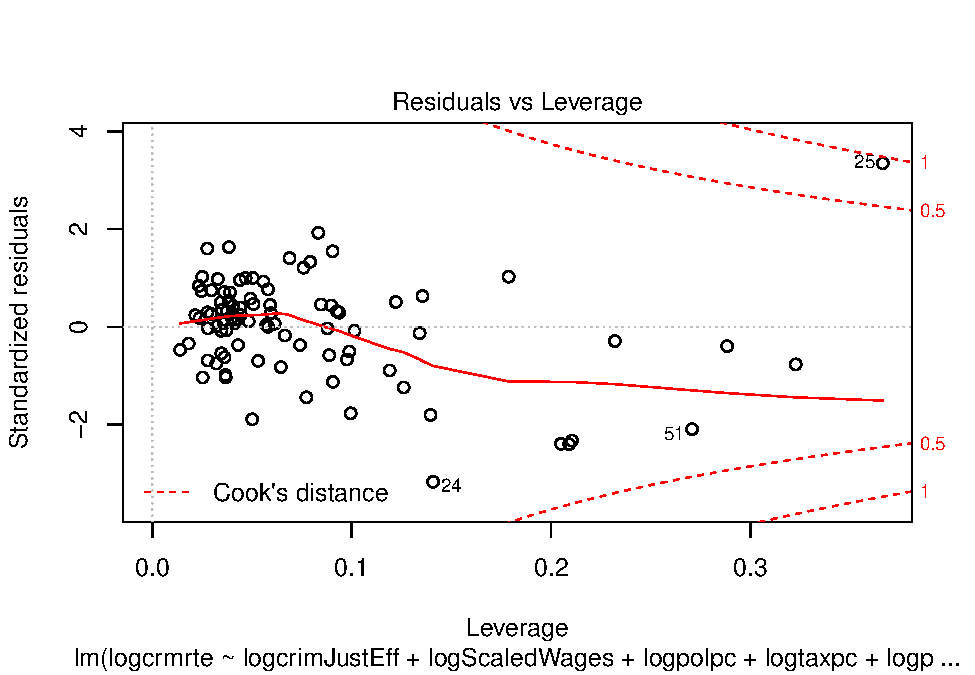
\includegraphics{Bagnard_Gaustad_Hartman_Leung_Lab_3_files/figure-latex/unnamed-chunk-84-1.pdf}

\textbf{Model 3 CLM Assumptions:}

\begin{itemize}
\item
  \textbf{MLR1 and 2}: Discussed earlier.
\item
  \textbf{MLR3} No perfect multicollinearity: We demonstrate that our
  independent variables are not perfectly multicollinear using the VIF
  function, and note that all of our variance inflation factors are less
  than 5.
\end{itemize}

\begin{Shaded}
\begin{Highlighting}[]
\KeywordTok{vif}\NormalTok{(model3)}
\end{Highlighting}
\end{Shaded}

\begin{verbatim}
## logcrimJustEff logScaledWages       logpolpc       logtaxpc    logpctmin80 
##       1.355465       1.807350       1.540045       1.387756       1.072159 
##        density 
##       2.150401
\end{verbatim}

\begin{itemize}
\tightlist
\item
  \textbf{MLR4'} Zero Conditional Mean: From the residual vs.~fitted
  chart below, we see that the mean of the residuals mostly lie along 0,
  except towards the right side of our chart where there are fewer data
  points. We can reasonably conclude that we satisfy MLR4.
\end{itemize}

\begin{Shaded}
\begin{Highlighting}[]
\KeywordTok{plot}\NormalTok{(model3, }\DataTypeTok{which =} \DecValTok{1}\NormalTok{)}
\end{Highlighting}
\end{Shaded}

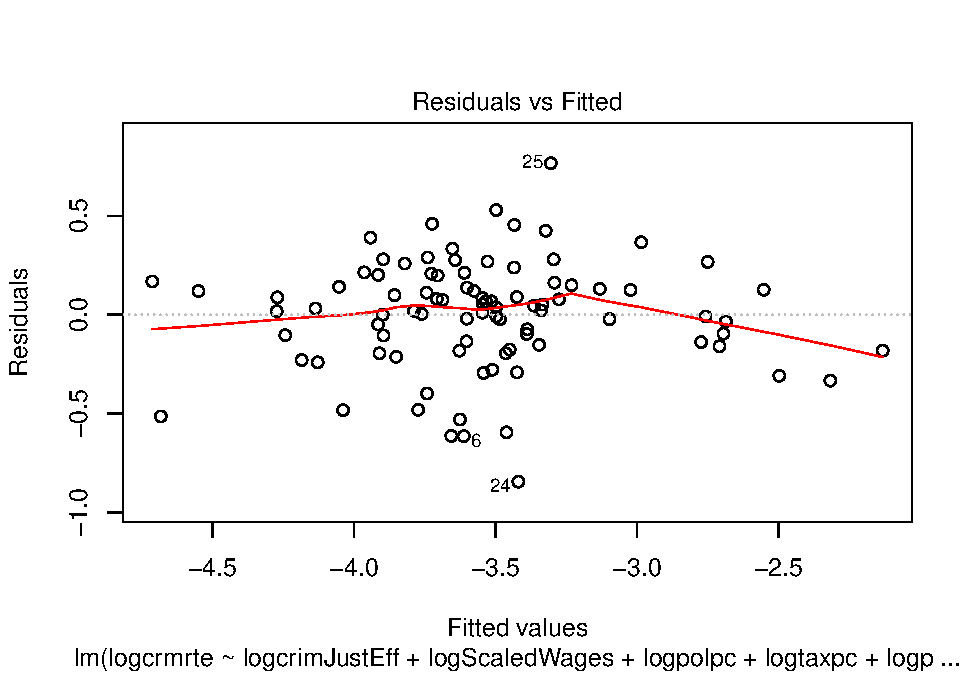
\includegraphics{Bagnard_Gaustad_Hartman_Leung_Lab_3_files/figure-latex/unnamed-chunk-86-1.pdf}

\begin{itemize}
\tightlist
\item
  \textbf{MLR5'} Spherical errors: We note from the residuals vs fitted
  chart above that we have some evidence of heteroscedasticity, since
  there are less datapoints on both the left and right of the chart. As
  a result, we use the vcovHC method to estimate a robust
  variance-covariance matrix using White and Huber's method and generate
  coefficients that are robust to heteroscedasticity. Given that the
  coefficients in our model are fairly small, we know that the robust
  coeffcients generated will be appropriate for our analysis.
\end{itemize}

\begin{Shaded}
\begin{Highlighting}[]
\KeywordTok{coeftest}\NormalTok{(model3, }\DataTypeTok{vcov=}\NormalTok{vcovHC)}
\end{Highlighting}
\end{Shaded}

\begin{verbatim}

t test of coefficients:

                Estimate Std. Error t value  Pr(>|t|)    
(Intercept)    -7.282959   4.471722 -1.6287   0.10717    
logcrimJustEff -0.434396   0.099117 -4.3827 3.407e-05 ***
logScaledWages  0.961884   0.620157  1.5510   0.12470    
logpolpc        0.315789   0.199327  1.5843   0.11693    
logtaxpc       -0.097502   0.290658 -0.3355   0.73813    
logpctmin80     0.256954   0.044956  5.7157 1.666e-07 ***
density         0.077021   0.040837  1.8861   0.06278 .  
---
Signif. codes:  0 '***' 0.001 '**' 0.01 '*' 0.05 '.' 0.1 ' ' 1
\end{verbatim}

\begin{itemize}
\tightlist
\item
  \textbf{MLR6'} Normality of errors: From the qqplot below, we see that
  the residuals in our model follow a fairly normal distribution. In
  addition, since we have a large sample size of 90 datapoints, we can
  rely on a version of the central limit theorem to assume normally
  distributed errors.
\end{itemize}

\begin{Shaded}
\begin{Highlighting}[]
\KeywordTok{plot}\NormalTok{(model3,}\DataTypeTok{which=}\DecValTok{2}\NormalTok{)}
\end{Highlighting}
\end{Shaded}

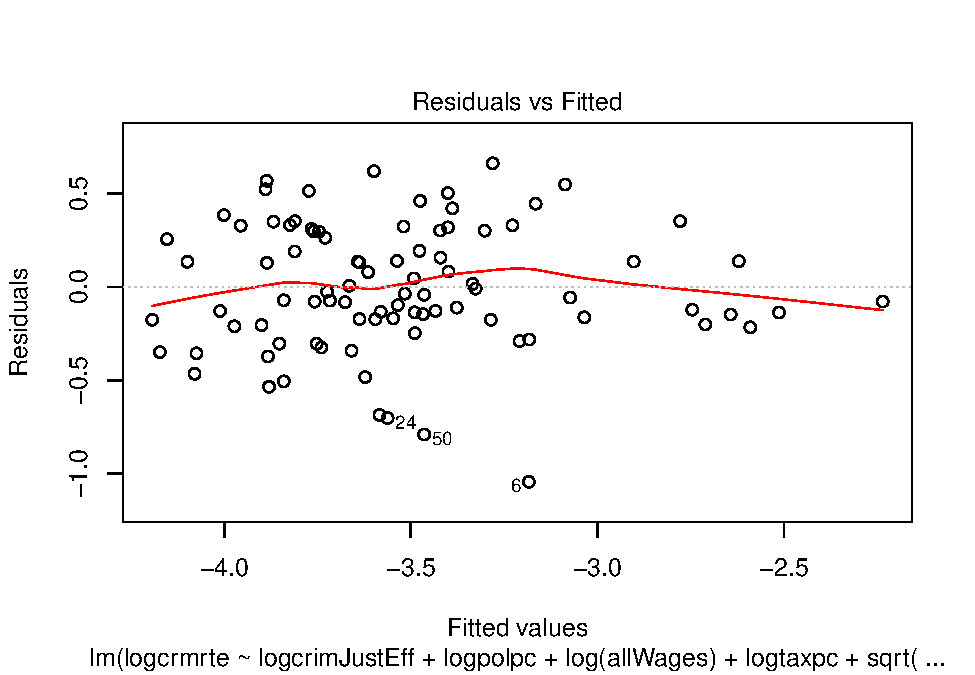
\includegraphics{Bagnard_Gaustad_Hartman_Leung_Lab_3_files/figure-latex/unnamed-chunk-88-1.pdf}

By satisfying these assumptions, we can expect that our coefficients are
approaching the true parameter values in probability.

\hypertarget{analysis}{%
\subsubsection{Analysis}\label{analysis}}

The model shows a good fit, with an adjusted R-squared of 0.72, meaning
that the model explains 72\% of the variation in crime.

After accounting for coefficients that are robust to heteroscedasticity,
we note only three them have individual statistical significance at the
95\% level or better. These are criminal justice efficiency, minority
percentages and density. However, running a F-test on the other two
variables logpolpc and logScaledWages show that jointly they are still
significant for our model.

\begin{Shaded}
\begin{Highlighting}[]
\KeywordTok{linearHypothesis}\NormalTok{(model3,}\KeywordTok{c}\NormalTok{(}\StringTok{"logpolpc=0"}\NormalTok{,}\StringTok{"logScaledWages=0"}\NormalTok{,}\StringTok{"logtaxpc=0"}\NormalTok{), }\DataTypeTok{vcov=}\NormalTok{vcovHC)}
\end{Highlighting}
\end{Shaded}

\begin{verbatim}
## Linear hypothesis test
## 
## Hypothesis:
## logpolpc = 0
## logScaledWages = 0
## logtaxpc = 0
## 
## Model 1: restricted model
## Model 2: logcrmrte ~ logcrimJustEff + logScaledWages + logpolpc + logtaxpc + 
##     logpctmin80 + density
## 
## Note: Coefficient covariance matrix supplied.
## 
##   Res.Df Df     F  Pr(>F)  
## 1     86                   
## 2     83  3 3.413 0.02118 *
## ---
## Signif. codes:  0 '***' 0.001 '**' 0.01 '*' 0.05 '.' 0.1 ' ' 1
\end{verbatim}

\textbf{Interpretation of coefficients (Assuming ceterus paribus):}

Positive coefficients: * Police presence: If we increase police per
capita by 1 percent, we expect the crime rate to increase by 0.28\%. *
scaledWages: If we increase wages by 1 percent, we expect the crime rate
to increase by 0.96\% * Density: If we increase density by 1 person per
square mile, we expect the crime rate to increase by 7.48\% * Percentage
of minorities: If the percentage of minorities increase by 1\%, we
expect the crime rate to increase by 0.25\%

Negative coefficients: * Criminal justice efficiency: If we increase the
criminal justice efficiency by 1\%, we expect the crime rate to decrease
by 0.43\%.

Of these different variables, we should pay particular attention to
density given its large practical effect and statistical significance,
which we address in our policy recommendations section below.

\hypertarget{comparison-of-regression-models}{%
\subsection{Comparison of Regression
Models}\label{comparison-of-regression-models}}

*\textbf{Can anyone figure out why logcrimJustEff is on 2 lines?}

\begin{Shaded}
\begin{Highlighting}[]
\CommentTok{#*** Function to convert coeftest results object into data frame}
\NormalTok{ctdf=}\ControlFlowTok{function}\NormalTok{(x)\{}
\NormalTok{  rt=}\KeywordTok{list}\NormalTok{()                             }\CommentTok{# generate empty results list}
  \ControlFlowTok{for}\NormalTok{(c }\ControlFlowTok{in} \DecValTok{1}\OperatorTok{:}\KeywordTok{dim}\NormalTok{(x)[}\DecValTok{2}\NormalTok{]) rt[[c]]=x[,c]   }\CommentTok{# writes column values of x to list}
\NormalTok{  rt=}\KeywordTok{as.data.frame}\NormalTok{(rt)                  }\CommentTok{# converts list to data frame object}
  \KeywordTok{names}\NormalTok{(rt)=}\KeywordTok{names}\NormalTok{(x[}\DecValTok{1}\NormalTok{,])                }\CommentTok{# assign correct column names}
\NormalTok{  rt[,}\StringTok{"sig"}\NormalTok{]=}\KeywordTok{symnum}\NormalTok{(rt}\OperatorTok{$}\StringTok{`}\DataTypeTok{Pr(>|z|)}\StringTok{`}\NormalTok{, }\DataTypeTok{corr =} \OtherTok{FALSE}\NormalTok{, }\DataTypeTok{na =} \OtherTok{FALSE}\NormalTok{,}
                    \DataTypeTok{cutpoints =} \KeywordTok{c}\NormalTok{(}\DecValTok{0}\NormalTok{, }\FloatTok{0.001}\NormalTok{, }\FloatTok{0.01}\NormalTok{, }\FloatTok{0.05}\NormalTok{, }\FloatTok{0.1}\NormalTok{, }\DecValTok{1}\NormalTok{),}
                    \DataTypeTok{symbols =} \KeywordTok{c}\NormalTok{(}\StringTok{"***"}\NormalTok{, }\StringTok{"**"}\NormalTok{, }\StringTok{"*"}\NormalTok{, }\StringTok{"."}\NormalTok{, }\StringTok{" "}\NormalTok{))}
  \KeywordTok{return}\NormalTok{(rt)}
\NormalTok{\}}
\CommentTok{# Get vectors of robust standard errors from the coeftest output}
\NormalTok{se.model1 <-}\StringTok{ }\KeywordTok{ctdf}\NormalTok{(}\KeywordTok{coeftest}\NormalTok{(mod1, }\DataTypeTok{vcov=}\NormalTok{vcovHC))[,}\StringTok{"Std. Error"}\NormalTok{]}
\NormalTok{se.model2 <-}\StringTok{ }\KeywordTok{ctdf}\NormalTok{(}\KeywordTok{coeftest}\NormalTok{(model2, }\DataTypeTok{vcov=}\NormalTok{vcovHC))[,}\StringTok{"Std. Error"}\NormalTok{]}
\CommentTok{#model23<-lm(logcrmrte ~ logcrimJustEff + logpolpc + logScaledWages + logpolpc*regcode + logtaxpc +density + logpctmin80, data = dfCrime)}
\CommentTok{#se.model23 <- ctdf(coeftest(model23, vcov=vcovHC))[,"Std. Error"]}
\NormalTok{se.model3 <-}\StringTok{ }\KeywordTok{ctdf}\NormalTok{(}\KeywordTok{coeftest}\NormalTok{(model3, }\DataTypeTok{vcov=}\NormalTok{vcovHC))[,}\StringTok{"Std. Error"}\NormalTok{]}
\CommentTok{# Pass the standard errors into stargazer}
\CommentTok{#stargazer(mod1, model2, model23, model3, type = "text", omit.stat = "f",}
\CommentTok{#          se = list(se.model1, se.model2, se.model23, se.model3),}
\CommentTok{#          star.cutoffs = c(0.05, 0.01, 0.001))}

\KeywordTok{stargazer}\NormalTok{(mod1, model2, model3, }\DataTypeTok{type =} \StringTok{"text"}\NormalTok{, }\DataTypeTok{omit.stat =} \StringTok{"f"}\NormalTok{,}
          \DataTypeTok{se =} \KeywordTok{list}\NormalTok{(se.model1, se.model2, se.model3),}
          \DataTypeTok{star.cutoffs =} \KeywordTok{c}\NormalTok{(}\FloatTok{0.05}\NormalTok{, }\FloatTok{0.01}\NormalTok{, }\FloatTok{0.001}\NormalTok{))}
\end{Highlighting}
\end{Shaded}

\begin{verbatim}

=======================================================================
                                      Dependent variable:              
                        -----------------------------------------------
                                           logcrmrte                   
                              (1)             (2)             (3)      
-----------------------------------------------------------------------
logScaledWages             1.998***         1.198*           0.962     
                            (0.487)         (0.471)         (0.620)    
                                                                       
logcrimJustEff             -0.480***       -0.423***       -0.434***   
                            (0.104)         (0.106)         (0.099)    
                                                                       
logpolpc                                    0.563*           0.316     
                                            (0.253)         (0.199)    
                                                                       
regcodeWest                -0.590***        -5.810*                    
                            (0.101)         (2.914)                    
                                                                       
regcodeCentral             -0.243**          0.999                     
                            (0.081)         (1.438)                    
                                                                       
logtaxpc                                    -0.154          -0.098     
                                            (0.190)         (0.291)    
                                                                       
logpolpc:regcodeWest                        -0.803                     
                                            (0.446)                    
                                                                       
logpolpc:regcodeCentral                      0.185                     
                                            (0.220)                    
                                                                       
logpctmin80                                                0.257***    
                                                            (0.045)    
                                                                       
density                                                      0.077     
                                                            (0.041)    
                                                                       
Constant                  -15.855***        -6.929          -7.283     
                            (2.660)         (3.592)         (4.472)    
                                                                       
-----------------------------------------------------------------------
Observations                  90              90              90       
R2                           0.652           0.728           0.744     
Adjusted R2                  0.636           0.702           0.726     
Residual Std. Error     0.331 (df = 85) 0.300 (df = 81) 0.287 (df = 83)
=======================================================================
Note:                                     *p<0.05; **p<0.01; ***p<0.001
\end{verbatim}

\begin{Shaded}
\begin{Highlighting}[]
\CommentTok{# waldtest(mod1, model2, vcov=vcovHC)}
\CommentTok{# waldtest(model2, model23, vcov=vcovHC)}
\CommentTok{# waldtest(model23, model3, vcov=vcovHC)}
\CommentTok{# }
\CommentTok{# model4<-lm(logcrmrte ~ logcrimJustEff + logpolpc + logScaledWages + logpolpc*west  +density + logpctmin80, data = dfCrime)}
\CommentTok{# coeftest(model4, vcov=vcovHC)}
\CommentTok{# summary(model4)$adj.r.square}
\CommentTok{# linearHypothesis(model4,c("logpolpc:west=0", "west=0"), vcov=vcovHC)}
\end{Highlighting}
\end{Shaded}

Comparing the 3 models, we see that our adjusted R2 value has steadily
increased from 0.456-0.732 as we introduce more covariates which
indicates that we were able to explain more variation in our model not
purely by increasing the number of indepedent variables.

At the same time, our standard errors have decreased \textbf{insert more
commentary on standard errors}.

We see that by expanding our definitions of criminal justice efficiency
and economic opportunity between model 1 and model 3 lowered the
coefficients for logcrimJustEff and scaledWages. This is most likely
because that we were able to better explain the effects with our newer
variables.

Comment on practical significance after week 12

\hypertarget{conclusion}{%
\section{Conclusion}\label{conclusion}}

\hypertarget{policy-recommendations}{%
\subsection{Policy Recommendations}\label{policy-recommendations}}

Given that across all 3 models, we show that both criminal justice
efficiency and tax revenues per capita have negative correlations to
crime rate, we propose the policy recommendations below to address these
issues. In addition, since minority percentages and density were found
to be highly significant in the model 3, we believe our recommendations
will be of particularly help to those running for political office in
counties with a high percentage of minorities or dense urban
populations.

\begin{enumerate}
\def\labelenumi{\arabic{enumi}.}
\item
  Since increasing both criminal justice and tax revenues are negatively
  correlated, we propose providing more funding for the local justice
  system.
\item
  While increasing taxes on constituents may be difficult politically
  and may cost candidates the ballot, candidates can instead try to
  attract investment to bring more jobs with higher wages so you can
  increase revenues.
\item
  Candidates can also propose to levy taxes on things that could lead to
  crimes or violence such as alcohol and weapons.
\item
  Given the significance and relatively large coefficient size of
  percentage minority, candidates should enroll local law enforcement
  into bias training.
\end{enumerate}

\hypertarget{ommitted-variables}{%
\subsection{Ommitted Variables}\label{ommitted-variables}}

\begin{longtable}[]{@{}l@{}}
\toprule
Expected correlation between omitted and included
variables\tabularnewline
\midrule
\endhead
\bottomrule
\end{longtable}

\begin{longtable}[]{@{}llll@{}}
\toprule
\begin{minipage}[b]{0.18\columnwidth}\raggedright
Omitted Variable\strut
\end{minipage} & \begin{minipage}[b]{0.19\columnwidth}\raggedright
Crime Rate (\(B_k\))\strut
\end{minipage} & \begin{minipage}[b]{0.31\columnwidth}\raggedright
Criminal Justice Effectiveness\strut
\end{minipage} & \begin{minipage}[b]{0.20\columnwidth}\raggedright
Economic Conditions\strut
\end{minipage}\tabularnewline
\midrule
\endhead
\begin{minipage}[t]{0.18\columnwidth}\raggedright
Education\strut
\end{minipage} & \begin{minipage}[t]{0.19\columnwidth}\raggedright
-\strut
\end{minipage} & \begin{minipage}[t]{0.31\columnwidth}\raggedright
unknown\strut
\end{minipage} & \begin{minipage}[t]{0.20\columnwidth}\raggedright
+\strut
\end{minipage}\tabularnewline
\begin{minipage}[t]{0.18\columnwidth}\raggedright
Social Services\strut
\end{minipage} & \begin{minipage}[t]{0.19\columnwidth}\raggedright
-\strut
\end{minipage} & \begin{minipage}[t]{0.31\columnwidth}\raggedright
unknown\strut
\end{minipage} & \begin{minipage}[t]{0.20\columnwidth}\raggedright
unknown\strut
\end{minipage}\tabularnewline
\begin{minipage}[t]{0.18\columnwidth}\raggedright
Unemployment\strut
\end{minipage} & \begin{minipage}[t]{0.19\columnwidth}\raggedright
+\strut
\end{minipage} & \begin{minipage}[t]{0.31\columnwidth}\raggedright
unknown\strut
\end{minipage} & \begin{minipage}[t]{0.20\columnwidth}\raggedright
-\strut
\end{minipage}\tabularnewline
\begin{minipage}[t]{0.18\columnwidth}\raggedright
Inequality\strut
\end{minipage} & \begin{minipage}[t]{0.19\columnwidth}\raggedright
+\strut
\end{minipage} & \begin{minipage}[t]{0.31\columnwidth}\raggedright
unknown\strut
\end{minipage} & \begin{minipage}[t]{0.20\columnwidth}\raggedright
-\strut
\end{minipage}\tabularnewline
\begin{minipage}[t]{0.18\columnwidth}\raggedright
Gang Activity\strut
\end{minipage} & \begin{minipage}[t]{0.19\columnwidth}\raggedright
+\strut
\end{minipage} & \begin{minipage}[t]{0.31\columnwidth}\raggedright
-\strut
\end{minipage} & \begin{minipage}[t]{0.20\columnwidth}\raggedright
-\strut
\end{minipage}\tabularnewline
\bottomrule
\end{longtable}

The 4 major identified ommited variables are shown above.

\begin{itemize}
\tightlist
\item
  Education is an important variable because of demographic insights it
  provides. First, adults with higher education are less likely to
  participate in Crime and are more likely to have better economic
  opportunity. Second, a strong school system is also likely correlated
  with less youth crime. Because of these expected correlations we are
  likely overestimating the economic conditions coefficient estimate.
\item
  Available Social Services could also lower crime. Citizens with strong
  social services support have more options to get help when they lack
  means for purchasing basic life needs. However this is more difficult
  to predict, as some social service projects, like homeless shelters,
  could lead to more criminal activity.
\item
  Unemployment is used as an important indicator of economic health and
  opportunity. This is would be highly correlated to economic conditions
  variables like sum of wages. This indicator variable if added to the
  model would decrease the magnitude of the sum of wage means
  coefficient estimate.\\
\item
  Economic Inequality may also increase the crime rate as it may provide
  incentives for certain types of crime such as theft, kidnapping or
  extortion by people who have less economic means on those who have
  more economic means.
\item
  Gang or Organized Crime is special case of crime that contains unique
  causes. It is expected that it would be negatively correlated with
  criminal justice effectiveness as large social pressures prevent
  witnesses from supporting prosecution. Gang crime is also negatively
  correlated with economic conditions. From these assumed correlations,
  we can say that criminal justice effectiveness and economic conditions
  are both underestimated compared to including gang activity
  operationalized variable in the model.
\end{itemize}

\hypertarget{research-recommendations}{%
\subsection{Research Recommendations}\label{research-recommendations}}

We have shown in this report 3 different models that seek to explain and
model changes in the crime rate in North Carolina in 1980. We start with
the fundamental premise that crime is caused by both criminal justice
efficiency and economic conditions, and further develop our definition
of these two key explanatory variables which each new model.

In Model 3, we were able to explain up to 73\% of the variation in our
data, and found statistical significance at the 95\% level or better for
each of our covariates. Of these, we believe that increasing the
efficiency of the criminal justice system and tax revenues were the most
important, particularly for counties with high density and minority
populations. However, our findings should be noted with caution as we
were unable to study the effect of several ommitted variables including
education, availability of social services, unemployment rates and the
presence of organized crime. Had we been able to collect data on these
variables and apply them in our model, we believe we could increase
accuracy without bias.

\hypertarget{appendix}{%
\section{Appendix}\label{appendix}}

\begin{Shaded}
\begin{Highlighting}[]
\KeywordTok{options}\NormalTok{(}\DataTypeTok{repr.plot.width=}\DecValTok{8}\NormalTok{, }\DataTypeTok{repr.plot.height=}\DecValTok{4}\NormalTok{)}
\CommentTok{#myData<-myData[, c("crmrte", "prbarr", "prbconv", "prbpris", "avgsen", "polpc", "density", "taxpc",}
\CommentTok{#           "pctmin80", "wcon", "wtuc", "wtrd", "wfir", "wser", "wmfg", "wfed", "wsta", "wloc",}
\CommentTok{#           "mix", "pctymle")]}
\NormalTok{myData<-dfCrime }\OperatorTok\StringTok{ }\KeywordTok{filter}\NormalTok{(other}\OperatorTok{==}\DecValTok{1}\NormalTok{)}
\NormalTok{myData<-myData[, }\KeywordTok{c}\NormalTok{(}\StringTok{"crmrte"}\NormalTok{, }\StringTok{"prbarr"}\NormalTok{, }\StringTok{"prbconv"}\NormalTok{, }\StringTok{"prbpris"}\NormalTok{, }\StringTok{"avgsen"}\NormalTok{, }\StringTok{"polpc"}\NormalTok{, }\StringTok{"density"}\NormalTok{, }\StringTok{"taxpc"}\NormalTok{,}
          \StringTok{"pctmin80"}\NormalTok{, }\StringTok{"wcon"}\NormalTok{, }\StringTok{"wtuc"}\NormalTok{, }\StringTok{"wtrd"}\NormalTok{, }\StringTok{"wfir"}\NormalTok{, }\StringTok{"wser"}\NormalTok{, }\StringTok{"wmfg"}\NormalTok{, }\StringTok{"wfed"}\NormalTok{, }\StringTok{"wsta"}\NormalTok{, }\StringTok{"wloc"}\NormalTok{,}
          \StringTok{"mix"}\NormalTok{, }\StringTok{"pctymle"}\NormalTok{)]}
\NormalTok{r0 <-}\StringTok{ }\NormalTok{myData }\OperatorTok\StringTok{ }\KeywordTok{correlate}\NormalTok{() }\OperatorTok\StringTok{ }\KeywordTok{network_plot}\NormalTok{(}\DataTypeTok{min_cor=}\NormalTok{.}\DecValTok{25}\NormalTok{)}
\end{Highlighting}
\end{Shaded}

\begin{verbatim}

Correlation method: 'pearson'
Missing treated using: 'pairwise.complete.obs'
\end{verbatim}

\begin{Shaded}
\begin{Highlighting}[]
\NormalTok{myData<-dfCrime }\OperatorTok\StringTok{ }\KeywordTok{filter}\NormalTok{(central}\OperatorTok{==}\DecValTok{1}\NormalTok{)}
\NormalTok{myData<-myData[, }\KeywordTok{c}\NormalTok{(}\StringTok{"crmrte"}\NormalTok{, }\StringTok{"prbarr"}\NormalTok{, }\StringTok{"prbconv"}\NormalTok{, }\StringTok{"prbpris"}\NormalTok{, }\StringTok{"avgsen"}\NormalTok{, }\StringTok{"polpc"}\NormalTok{, }\StringTok{"density"}\NormalTok{, }\StringTok{"taxpc"}\NormalTok{,}
          \StringTok{"pctmin80"}\NormalTok{, }\StringTok{"wcon"}\NormalTok{, }\StringTok{"wtuc"}\NormalTok{, }\StringTok{"wtrd"}\NormalTok{, }\StringTok{"wfir"}\NormalTok{, }\StringTok{"wser"}\NormalTok{, }\StringTok{"wmfg"}\NormalTok{, }\StringTok{"wfed"}\NormalTok{, }\StringTok{"wsta"}\NormalTok{, }\StringTok{"wloc"}\NormalTok{,}
          \StringTok{"mix"}\NormalTok{, }\StringTok{"pctymle"}\NormalTok{)]}
\NormalTok{r1 <-}\StringTok{ }\NormalTok{myData }\OperatorTok\StringTok{ }\KeywordTok{correlate}\NormalTok{() }\OperatorTok\StringTok{ }\KeywordTok{network_plot}\NormalTok{(}\DataTypeTok{min_cor=}\NormalTok{.}\DecValTok{25}\NormalTok{)}
\end{Highlighting}
\end{Shaded}

\begin{verbatim}

Correlation method: 'pearson'
Missing treated using: 'pairwise.complete.obs'
\end{verbatim}

\begin{Shaded}
\begin{Highlighting}[]
\NormalTok{myData<-dfCrime }\OperatorTok\StringTok{ }\KeywordTok{filter}\NormalTok{(west}\OperatorTok{==}\DecValTok{1}\NormalTok{)}
\NormalTok{myData<-myData[, }\KeywordTok{c}\NormalTok{(}\StringTok{"crmrte"}\NormalTok{, }\StringTok{"prbarr"}\NormalTok{, }\StringTok{"prbconv"}\NormalTok{, }\StringTok{"prbpris"}\NormalTok{, }\StringTok{"avgsen"}\NormalTok{, }\StringTok{"polpc"}\NormalTok{, }\StringTok{"density"}\NormalTok{, }\StringTok{"taxpc"}\NormalTok{,}
          \StringTok{"pctmin80"}\NormalTok{, }\StringTok{"wcon"}\NormalTok{, }\StringTok{"wtuc"}\NormalTok{, }\StringTok{"wtrd"}\NormalTok{, }\StringTok{"wfir"}\NormalTok{, }\StringTok{"wser"}\NormalTok{, }\StringTok{"wmfg"}\NormalTok{, }\StringTok{"wfed"}\NormalTok{, }\StringTok{"wsta"}\NormalTok{, }\StringTok{"wloc"}\NormalTok{,}
          \StringTok{"mix"}\NormalTok{, }\StringTok{"pctymle"}\NormalTok{)]}
\NormalTok{r2 <-}\StringTok{ }\NormalTok{myData }\OperatorTok\StringTok{ }\KeywordTok{correlate}\NormalTok{() }\OperatorTok\StringTok{ }\KeywordTok{network_plot}\NormalTok{(}\DataTypeTok{min_cor=}\NormalTok{.}\DecValTok{25}\NormalTok{)}
\end{Highlighting}
\end{Shaded}

\begin{verbatim}

Correlation method: 'pearson'
Missing treated using: 'pairwise.complete.obs'
\end{verbatim}

\begin{Shaded}
\begin{Highlighting}[]
\KeywordTok{grid.arrange}\NormalTok{(}\KeywordTok{arrangeGrob}\NormalTok{(r1, }\DataTypeTok{bottom =} \StringTok{'Central Region Correlation Plot'}\NormalTok{), }\DataTypeTok{ncol=}\DecValTok{1}\NormalTok{)}
\end{Highlighting}
\end{Shaded}

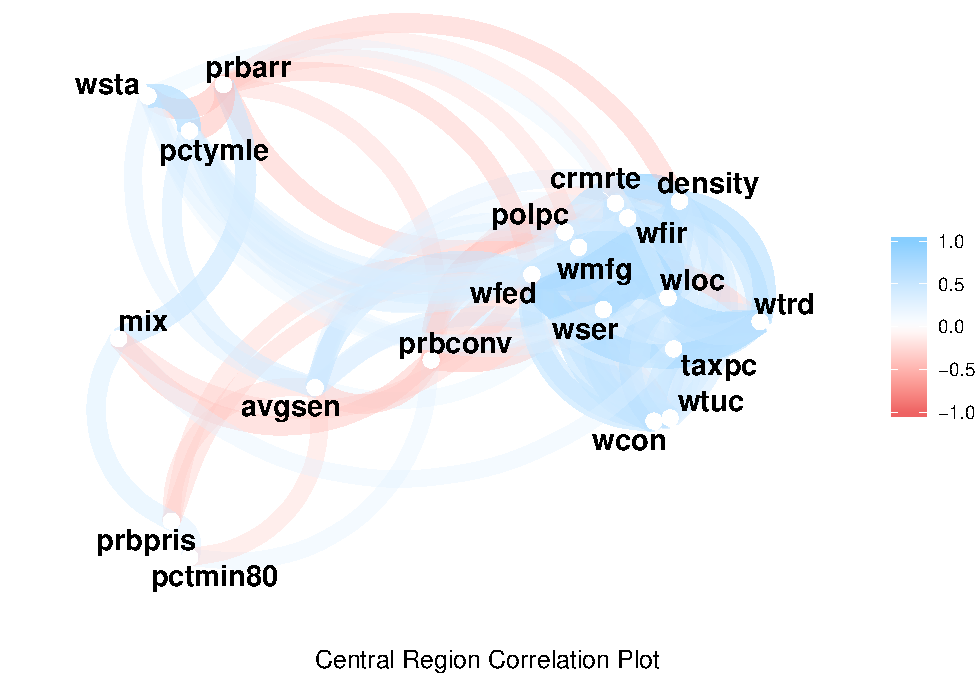
\includegraphics{Bagnard_Gaustad_Hartman_Leung_Lab_3_files/figure-latex/unnamed-chunk-91-1.pdf}

\begin{Shaded}
\begin{Highlighting}[]
\KeywordTok{grid.arrange}\NormalTok{(}\KeywordTok{arrangeGrob}\NormalTok{(r2, }\DataTypeTok{bottom =} \StringTok{'Western Region Correlation Plot'}\NormalTok{), }\DataTypeTok{ncol=}\DecValTok{1}\NormalTok{)}
\end{Highlighting}
\end{Shaded}

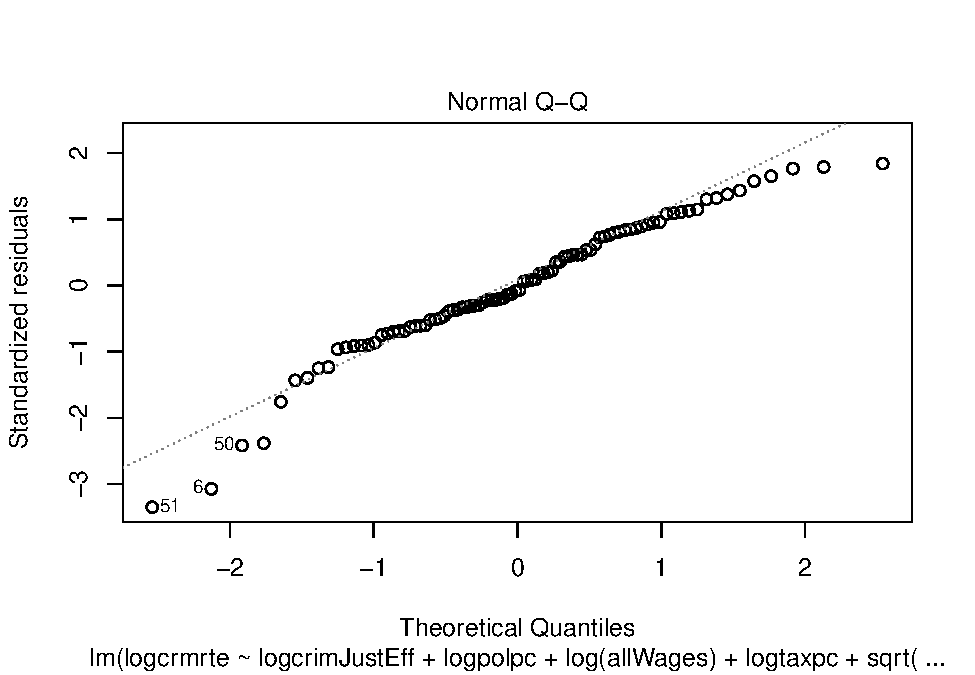
\includegraphics{Bagnard_Gaustad_Hartman_Leung_Lab_3_files/figure-latex/unnamed-chunk-91-2.pdf}

\begin{Shaded}
\begin{Highlighting}[]
\KeywordTok{grid.arrange}\NormalTok{(}\KeywordTok{arrangeGrob}\NormalTok{(r0, }\DataTypeTok{bottom =} \StringTok{'Other Region Correlation Plot'}\NormalTok{), }\DataTypeTok{ncol=}\DecValTok{1}\NormalTok{)}
\end{Highlighting}
\end{Shaded}

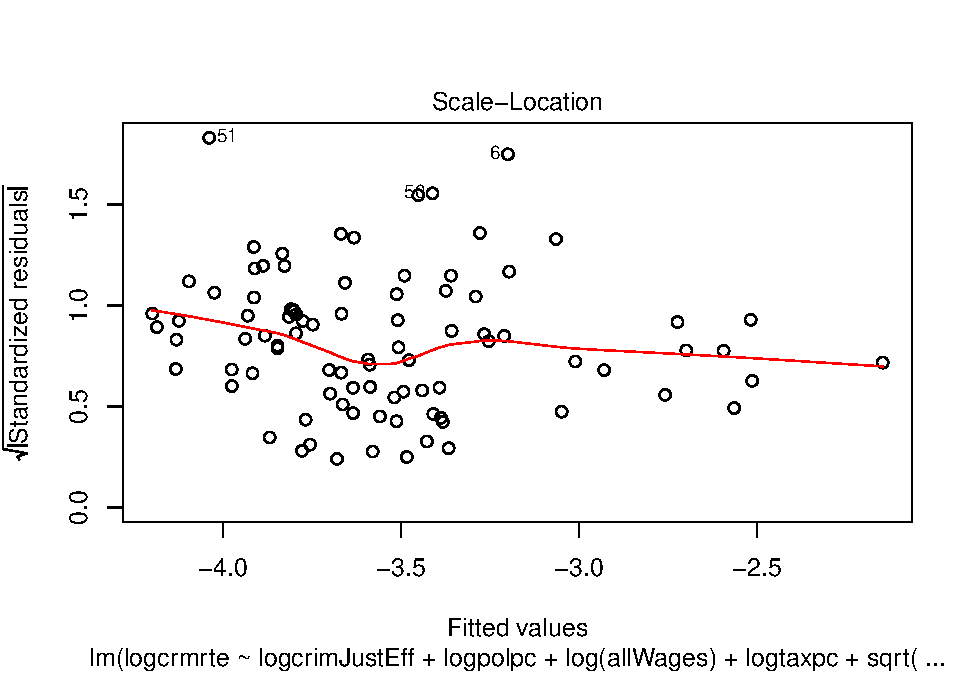
\includegraphics{Bagnard_Gaustad_Hartman_Leung_Lab_3_files/figure-latex/unnamed-chunk-91-3.pdf}

\begin{Shaded}
\begin{Highlighting}[]
\NormalTok{myData<-dfCrime }\OperatorTok\StringTok{ }\KeywordTok{filter}\NormalTok{(urban}\OperatorTok{==}\DecValTok{0}\NormalTok{)}
\NormalTok{myData<-myData[, }\KeywordTok{c}\NormalTok{(}\StringTok{"crmrte"}\NormalTok{, }\StringTok{"prbarr"}\NormalTok{, }\StringTok{"prbconv"}\NormalTok{, }\StringTok{"prbpris"}\NormalTok{, }\StringTok{"avgsen"}\NormalTok{, }\StringTok{"polpc"}\NormalTok{, }\StringTok{"density"}\NormalTok{, }\StringTok{"taxpc"}\NormalTok{,}
          \StringTok{"pctmin80"}\NormalTok{, }\StringTok{"wcon"}\NormalTok{, }\StringTok{"wtuc"}\NormalTok{, }\StringTok{"wtrd"}\NormalTok{, }\StringTok{"wfir"}\NormalTok{, }\StringTok{"wser"}\NormalTok{, }\StringTok{"wmfg"}\NormalTok{, }\StringTok{"wfed"}\NormalTok{, }\StringTok{"wsta"}\NormalTok{, }\StringTok{"wloc"}\NormalTok{,}
          \StringTok{"mix"}\NormalTok{, }\StringTok{"pctymle"}\NormalTok{)]}
\NormalTok{r0 <-}\StringTok{ }\NormalTok{myData }\OperatorTok\StringTok{ }\KeywordTok{correlate}\NormalTok{() }\OperatorTok\StringTok{ }\KeywordTok{network_plot}\NormalTok{(}\DataTypeTok{min_cor=}\NormalTok{.}\DecValTok{25}\NormalTok{)}
\end{Highlighting}
\end{Shaded}

\begin{verbatim}

Correlation method: 'pearson'
Missing treated using: 'pairwise.complete.obs'
\end{verbatim}

\begin{Shaded}
\begin{Highlighting}[]
\NormalTok{myData<-dfCrime }\OperatorTok\StringTok{ }\KeywordTok{filter}\NormalTok{(urban}\OperatorTok{==}\DecValTok{1}\NormalTok{)}
\NormalTok{myData<-myData[, }\KeywordTok{c}\NormalTok{(}\StringTok{"crmrte"}\NormalTok{, }\StringTok{"prbarr"}\NormalTok{, }\StringTok{"prbconv"}\NormalTok{, }\StringTok{"prbpris"}\NormalTok{, }\StringTok{"avgsen"}\NormalTok{, }\StringTok{"polpc"}\NormalTok{, }\StringTok{"density"}\NormalTok{, }\StringTok{"taxpc"}\NormalTok{,}
          \StringTok{"pctmin80"}\NormalTok{, }\StringTok{"wcon"}\NormalTok{, }\StringTok{"wtuc"}\NormalTok{, }\StringTok{"wtrd"}\NormalTok{, }\StringTok{"wfir"}\NormalTok{, }\StringTok{"wser"}\NormalTok{, }\StringTok{"wmfg"}\NormalTok{, }\StringTok{"wfed"}\NormalTok{, }\StringTok{"wsta"}\NormalTok{, }\StringTok{"wloc"}\NormalTok{,}
          \StringTok{"mix"}\NormalTok{, }\StringTok{"pctymle"}\NormalTok{)]}
\NormalTok{r1 <-}\StringTok{ }\NormalTok{myData }\OperatorTok\StringTok{ }\KeywordTok{correlate}\NormalTok{() }\OperatorTok\StringTok{ }\KeywordTok{network_plot}\NormalTok{(}\DataTypeTok{min_cor=}\NormalTok{.}\DecValTok{25}\NormalTok{)}
\end{Highlighting}
\end{Shaded}

\begin{verbatim}

Correlation method: 'pearson'
Missing treated using: 'pairwise.complete.obs'
\end{verbatim}

\begin{Shaded}
\begin{Highlighting}[]
\KeywordTok{grid.arrange}\NormalTok{(}\KeywordTok{arrangeGrob}\NormalTok{(r0, }\DataTypeTok{bottom =} \StringTok{'Non-Urban Correlation Plot'}\NormalTok{), }\DataTypeTok{ncol=}\DecValTok{1}\NormalTok{)}
\end{Highlighting}
\end{Shaded}

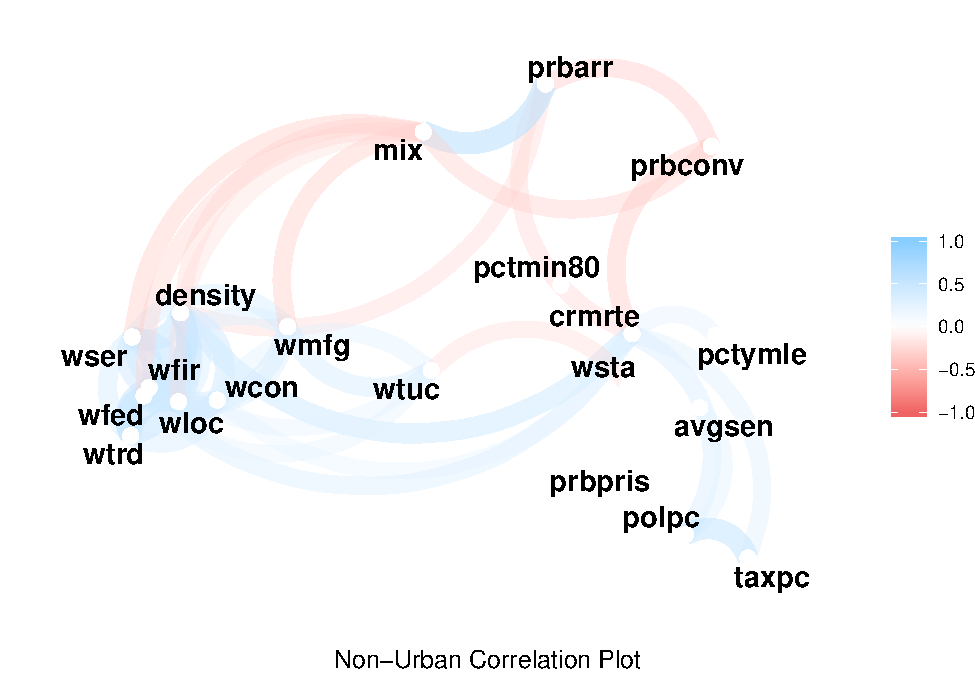
\includegraphics{Bagnard_Gaustad_Hartman_Leung_Lab_3_files/figure-latex/unnamed-chunk-91-4.pdf}

\begin{Shaded}
\begin{Highlighting}[]
\KeywordTok{grid.arrange}\NormalTok{(}\KeywordTok{arrangeGrob}\NormalTok{(r1, }\DataTypeTok{bottom =} \StringTok{'Urban Correlation Plot'}\NormalTok{), }\DataTypeTok{ncol=}\DecValTok{1}\NormalTok{)}
\end{Highlighting}
\end{Shaded}

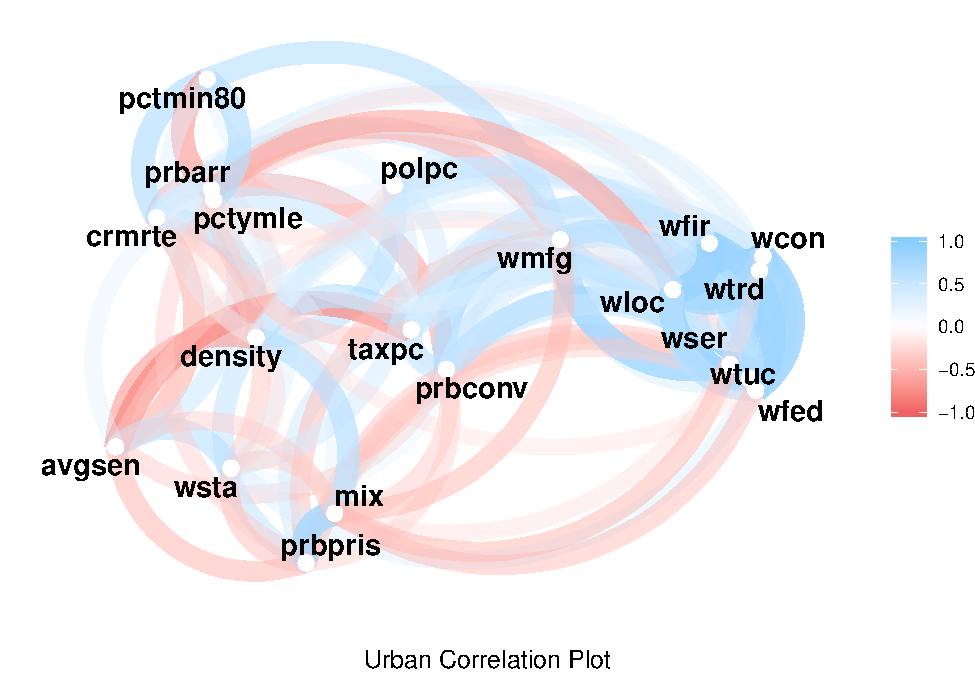
\includegraphics{Bagnard_Gaustad_Hartman_Leung_Lab_3_files/figure-latex/unnamed-chunk-91-5.pdf}

\hypertarget{transformations}{%
\subsection{Transformations}\label{transformations}}

Transform examinations through ggplots. Feel free to cherry pick what
you need. All of these plots will be removed in the final report.

\begin{Shaded}
\begin{Highlighting}[]
\CommentTok{#dfEconVars <- as.data.frame(cbind(dfCrime$wcon, dfCrime$wtuc, dfCrime$wtrd, dfCrime$wfir, }
\CommentTok{#                                  dfCrime$wser, dfCrime$wmfg, dfCrime$wfed, dfCrime$wsta, }
\CommentTok{#                                  dfCrime$wloc))}
\CommentTok{#names(dfEconVars) <- c('wcon', 'wtuc', 'wtrd', 'wfir', 'wser', }
\CommentTok{#                              'wmfg', 'wfed', 'wsta', 'wloc')}
\CommentTok{#}
\CommentTok{#ggplot(melt(dfEconVars),aes(x=value)) + geom_histogram(bins=30) + facet_wrap(~variable)}

\CommentTok{#The economic variables}
\NormalTok{q1<-}\KeywordTok{ggplot}\NormalTok{(}\DataTypeTok{data =}\NormalTok{ dfCrime, }\KeywordTok{aes}\NormalTok{(}\DataTypeTok{x =}\NormalTok{ wcon, }\DataTypeTok{y =}\NormalTok{ crmrte, }\DataTypeTok{color =}\NormalTok{ metro)) }\OperatorTok{+}\StringTok{ }
\StringTok{      }\KeywordTok{geom_point}\NormalTok{()}\OperatorTok{+}
\StringTok{  }\KeywordTok{geom_smooth}\NormalTok{(}\DataTypeTok{method =} \StringTok{"lm"}\NormalTok{)}
\NormalTok{q1a<-}\KeywordTok{ggplot}\NormalTok{(}\DataTypeTok{data =}\NormalTok{ dfCrime, }\KeywordTok{aes}\NormalTok{(}\DataTypeTok{x =} \KeywordTok{log}\NormalTok{(wcon), }\DataTypeTok{y =} \KeywordTok{log}\NormalTok{(crmrte), }\DataTypeTok{color =}\NormalTok{ metro)) }\OperatorTok{+}\StringTok{ }
\StringTok{      }\KeywordTok{geom_point}\NormalTok{()}\OperatorTok{+}
\StringTok{  }\KeywordTok{geom_smooth}\NormalTok{(}\DataTypeTok{method =} \StringTok{"lm"}\NormalTok{)}
\NormalTok{q2<-}\KeywordTok{ggplot}\NormalTok{(}\DataTypeTok{data =}\NormalTok{ dfCrime, }\KeywordTok{aes}\NormalTok{(}\DataTypeTok{x =}\NormalTok{ wtuc, }\DataTypeTok{y =}\NormalTok{ crmrte, }\DataTypeTok{color =}\NormalTok{ metro)) }\OperatorTok{+}\StringTok{ }
\StringTok{      }\KeywordTok{geom_point}\NormalTok{()}\OperatorTok{+}
\StringTok{  }\KeywordTok{geom_smooth}\NormalTok{(}\DataTypeTok{method =} \StringTok{"lm"}\NormalTok{)}
\NormalTok{q2a<-}\KeywordTok{ggplot}\NormalTok{(}\DataTypeTok{data =}\NormalTok{ dfCrime, }\KeywordTok{aes}\NormalTok{(}\DataTypeTok{x =} \KeywordTok{log}\NormalTok{(wtuc), }\DataTypeTok{y =} \KeywordTok{log}\NormalTok{(crmrte), }\DataTypeTok{color =}\NormalTok{ metro)) }\OperatorTok{+}\StringTok{ }
\StringTok{      }\KeywordTok{geom_point}\NormalTok{()}\OperatorTok{+}
\StringTok{  }\KeywordTok{geom_smooth}\NormalTok{(}\DataTypeTok{method =} \StringTok{"lm"}\NormalTok{)}
\NormalTok{q3<-}\KeywordTok{ggplot}\NormalTok{(}\DataTypeTok{data =}\NormalTok{ dfCrime, }\KeywordTok{aes}\NormalTok{(}\DataTypeTok{x =}\NormalTok{ wtrd, }\DataTypeTok{y =}\NormalTok{ crmrte, }\DataTypeTok{color =}\NormalTok{ metro)) }\OperatorTok{+}\StringTok{ }
\StringTok{      }\KeywordTok{geom_point}\NormalTok{()}\OperatorTok{+}
\StringTok{  }\KeywordTok{geom_smooth}\NormalTok{(}\DataTypeTok{method =} \StringTok{"lm"}\NormalTok{)}
\NormalTok{q3a<-}\KeywordTok{ggplot}\NormalTok{(}\DataTypeTok{data =}\NormalTok{ dfCrime, }\KeywordTok{aes}\NormalTok{(}\DataTypeTok{x =} \KeywordTok{log}\NormalTok{(wtrd), }\DataTypeTok{y =} \KeywordTok{log}\NormalTok{(crmrte), }\DataTypeTok{color =}\NormalTok{ metro)) }\OperatorTok{+}\StringTok{ }
\StringTok{      }\KeywordTok{geom_point}\NormalTok{()}\OperatorTok{+}
\StringTok{  }\KeywordTok{geom_smooth}\NormalTok{(}\DataTypeTok{method =} \StringTok{"lm"}\NormalTok{)}
\NormalTok{q4<-}\KeywordTok{ggplot}\NormalTok{(}\DataTypeTok{data =}\NormalTok{ dfCrime, }\KeywordTok{aes}\NormalTok{(}\DataTypeTok{x =}\NormalTok{ wfir, }\DataTypeTok{y =}\NormalTok{ crmrte, }\DataTypeTok{color =}\NormalTok{ metro)) }\OperatorTok{+}\StringTok{ }
\StringTok{      }\KeywordTok{geom_point}\NormalTok{()}\OperatorTok{+}
\StringTok{  }\KeywordTok{geom_smooth}\NormalTok{(}\DataTypeTok{method =} \StringTok{"lm"}\NormalTok{)}
\NormalTok{q4a<-}\KeywordTok{ggplot}\NormalTok{(}\DataTypeTok{data =}\NormalTok{ dfCrime, }\KeywordTok{aes}\NormalTok{(}\DataTypeTok{x =} \KeywordTok{log}\NormalTok{(wfir), }\DataTypeTok{y =} \KeywordTok{log}\NormalTok{(crmrte), }\DataTypeTok{color =}\NormalTok{ metro)) }\OperatorTok{+}\StringTok{ }
\StringTok{      }\KeywordTok{geom_point}\NormalTok{()}\OperatorTok{+}
\StringTok{  }\KeywordTok{geom_smooth}\NormalTok{(}\DataTypeTok{method =} \StringTok{"lm"}\NormalTok{)}
\NormalTok{q5<-}\KeywordTok{ggplot}\NormalTok{(}\DataTypeTok{data =}\NormalTok{ dfCrime, }\KeywordTok{aes}\NormalTok{(}\DataTypeTok{x =}\NormalTok{ wser, }\DataTypeTok{y =}\NormalTok{ crmrte, }\DataTypeTok{color =}\NormalTok{ metro)) }\OperatorTok{+}\StringTok{ }
\StringTok{      }\KeywordTok{geom_point}\NormalTok{()}\OperatorTok{+}
\StringTok{  }\KeywordTok{geom_smooth}\NormalTok{(}\DataTypeTok{method =} \StringTok{"lm"}\NormalTok{)}
\NormalTok{q5a<-}\KeywordTok{ggplot}\NormalTok{(}\DataTypeTok{data =}\NormalTok{ dfCrime, }\KeywordTok{aes}\NormalTok{(}\DataTypeTok{x =} \KeywordTok{log}\NormalTok{(wser), }\DataTypeTok{y =} \KeywordTok{log}\NormalTok{(crmrte), }\DataTypeTok{color =}\NormalTok{ metro)) }\OperatorTok{+}\StringTok{ }
\StringTok{      }\KeywordTok{geom_point}\NormalTok{()}\OperatorTok{+}
\StringTok{  }\KeywordTok{geom_smooth}\NormalTok{(}\DataTypeTok{method =} \StringTok{"lm"}\NormalTok{)}
\NormalTok{q6<-}\KeywordTok{ggplot}\NormalTok{(}\DataTypeTok{data =}\NormalTok{ dfCrime, }\KeywordTok{aes}\NormalTok{(}\DataTypeTok{x =}\NormalTok{ wmfg, }\DataTypeTok{y =}\NormalTok{ crmrte, }\DataTypeTok{color =}\NormalTok{ metro)) }\OperatorTok{+}\StringTok{ }
\StringTok{      }\KeywordTok{geom_point}\NormalTok{()}\OperatorTok{+}
\StringTok{  }\KeywordTok{geom_smooth}\NormalTok{(}\DataTypeTok{method =} \StringTok{"lm"}\NormalTok{)}
\NormalTok{q6a<-}\KeywordTok{ggplot}\NormalTok{(}\DataTypeTok{data =}\NormalTok{ dfCrime, }\KeywordTok{aes}\NormalTok{(}\DataTypeTok{x =} \KeywordTok{log}\NormalTok{(wmfg), }\DataTypeTok{y =} \KeywordTok{log}\NormalTok{(crmrte), }\DataTypeTok{color =}\NormalTok{ metro)) }\OperatorTok{+}\StringTok{ }
\StringTok{      }\KeywordTok{geom_point}\NormalTok{()}\OperatorTok{+}
\StringTok{  }\KeywordTok{geom_smooth}\NormalTok{(}\DataTypeTok{method =} \StringTok{"lm"}\NormalTok{)}
\NormalTok{q7<-}\KeywordTok{ggplot}\NormalTok{(}\DataTypeTok{data =}\NormalTok{ dfCrime, }\KeywordTok{aes}\NormalTok{(}\DataTypeTok{x =}\NormalTok{ wfed, }\DataTypeTok{y =}\NormalTok{ crmrte, }\DataTypeTok{color =}\NormalTok{ metro)) }\OperatorTok{+}\StringTok{ }
\StringTok{      }\KeywordTok{geom_point}\NormalTok{()}\OperatorTok{+}
\StringTok{  }\KeywordTok{geom_smooth}\NormalTok{(}\DataTypeTok{method =} \StringTok{"lm"}\NormalTok{)}
\NormalTok{q7a<-}\KeywordTok{ggplot}\NormalTok{(}\DataTypeTok{data =}\NormalTok{ dfCrime, }\KeywordTok{aes}\NormalTok{(}\DataTypeTok{x =} \KeywordTok{log}\NormalTok{(wfed), }\DataTypeTok{y =} \KeywordTok{log}\NormalTok{(crmrte), }\DataTypeTok{color =}\NormalTok{ metro)) }\OperatorTok{+}\StringTok{ }
\StringTok{      }\KeywordTok{geom_point}\NormalTok{()}\OperatorTok{+}
\StringTok{  }\KeywordTok{geom_smooth}\NormalTok{(}\DataTypeTok{method =} \StringTok{"lm"}\NormalTok{)}
\NormalTok{q8<-}\KeywordTok{ggplot}\NormalTok{(}\DataTypeTok{data =}\NormalTok{ dfCrime, }\KeywordTok{aes}\NormalTok{(}\DataTypeTok{x =}\NormalTok{ wsta, }\DataTypeTok{y =}\NormalTok{ crmrte, }\DataTypeTok{color =}\NormalTok{ metro)) }\OperatorTok{+}\StringTok{ }
\StringTok{      }\KeywordTok{geom_point}\NormalTok{()}\OperatorTok{+}
\StringTok{  }\KeywordTok{geom_smooth}\NormalTok{(}\DataTypeTok{method =} \StringTok{"lm"}\NormalTok{)}
\NormalTok{q8a<-}\KeywordTok{ggplot}\NormalTok{(}\DataTypeTok{data =}\NormalTok{ dfCrime, }\KeywordTok{aes}\NormalTok{(}\DataTypeTok{x =} \KeywordTok{log}\NormalTok{(wsta), }\DataTypeTok{y =} \KeywordTok{log}\NormalTok{(crmrte), }\DataTypeTok{color =}\NormalTok{ metro)) }\OperatorTok{+}\StringTok{ }
\StringTok{      }\KeywordTok{geom_point}\NormalTok{()}\OperatorTok{+}
\StringTok{  }\KeywordTok{geom_smooth}\NormalTok{(}\DataTypeTok{method =} \StringTok{"lm"}\NormalTok{)}
\NormalTok{q9<-}\KeywordTok{ggplot}\NormalTok{(}\DataTypeTok{data =}\NormalTok{ dfCrime, }\KeywordTok{aes}\NormalTok{(}\DataTypeTok{x =}\NormalTok{ wloc, }\DataTypeTok{y =}\NormalTok{ crmrte, }\DataTypeTok{color =}\NormalTok{ metro)) }\OperatorTok{+}\StringTok{ }
\StringTok{      }\KeywordTok{geom_point}\NormalTok{()}\OperatorTok{+}
\StringTok{  }\KeywordTok{geom_smooth}\NormalTok{(}\DataTypeTok{method =} \StringTok{"lm"}\NormalTok{)}
\NormalTok{q9a<-}\KeywordTok{ggplot}\NormalTok{(}\DataTypeTok{data =}\NormalTok{ dfCrime, }\KeywordTok{aes}\NormalTok{(}\DataTypeTok{x =} \KeywordTok{log}\NormalTok{(wloc), }\DataTypeTok{y =} \KeywordTok{log}\NormalTok{(crmrte), }\DataTypeTok{color =}\NormalTok{ metro)) }\OperatorTok{+}\StringTok{ }
\StringTok{      }\KeywordTok{geom_point}\NormalTok{()}\OperatorTok{+}
\StringTok{  }\KeywordTok{geom_smooth}\NormalTok{(}\DataTypeTok{method =} \StringTok{"lm"}\NormalTok{)}

\KeywordTok{options}\NormalTok{(}\DataTypeTok{repr.plot.width=}\DecValTok{8}\NormalTok{, }\DataTypeTok{repr.plot.height=}\DecValTok{16}\NormalTok{)}
\KeywordTok{grid.arrange}\NormalTok{(q1, q1a, q2, q2a, q3, q3a, }\DataTypeTok{ncol=}\DecValTok{2}\NormalTok{)}
\end{Highlighting}
\end{Shaded}

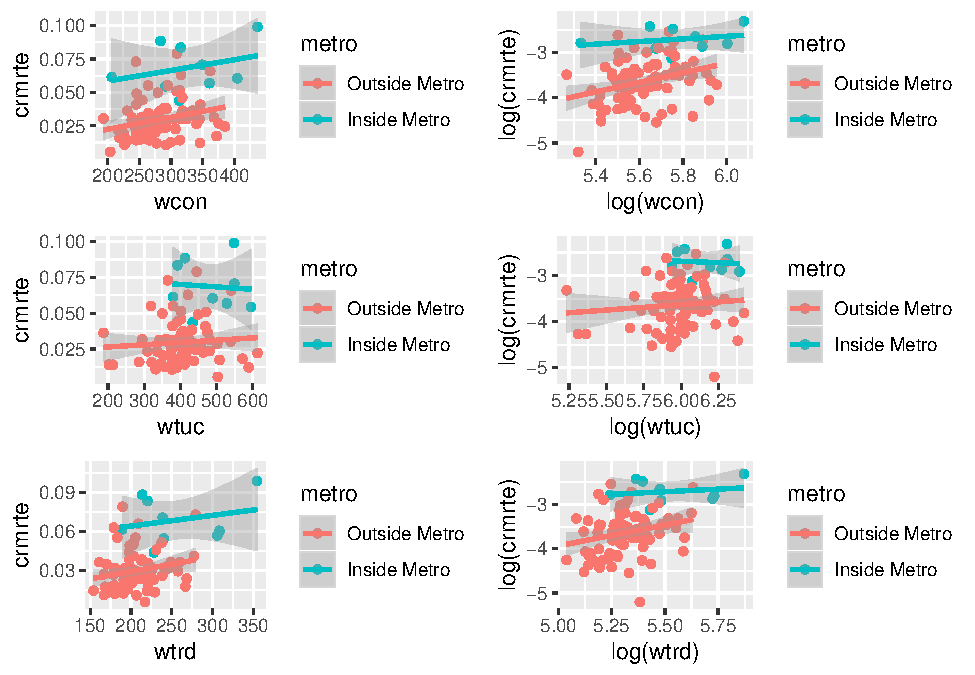
\includegraphics{Bagnard_Gaustad_Hartman_Leung_Lab_3_files/figure-latex/unnamed-chunk-92-1.pdf}

\begin{Shaded}
\begin{Highlighting}[]
\KeywordTok{grid.arrange}\NormalTok{(q4, q4a, q5, q5a, q6, q6a, }\DataTypeTok{ncol=}\DecValTok{2}\NormalTok{)}
\end{Highlighting}
\end{Shaded}

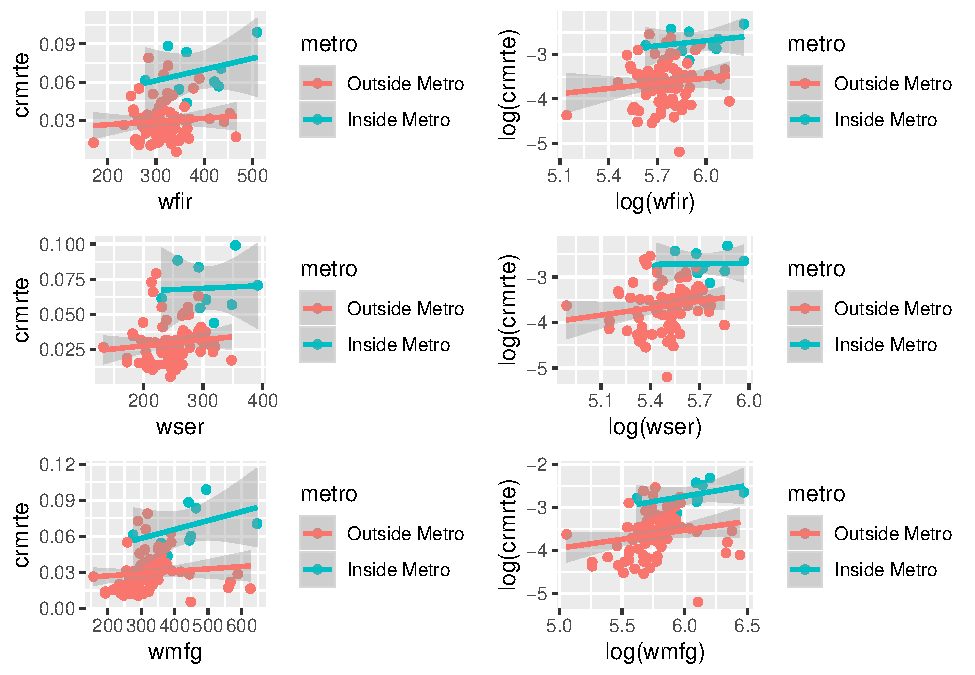
\includegraphics{Bagnard_Gaustad_Hartman_Leung_Lab_3_files/figure-latex/unnamed-chunk-92-2.pdf}

\begin{Shaded}
\begin{Highlighting}[]
\KeywordTok{grid.arrange}\NormalTok{(q7, q7a, q8, q8a, q9, q9a, }\DataTypeTok{ncol=}\DecValTok{2}\NormalTok{)}
\end{Highlighting}
\end{Shaded}

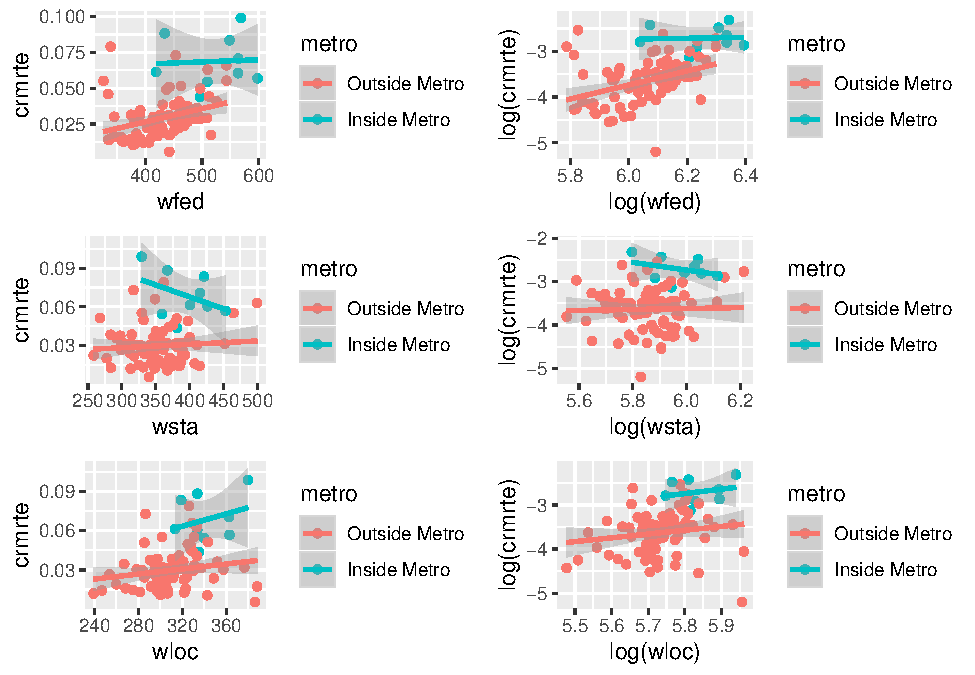
\includegraphics{Bagnard_Gaustad_Hartman_Leung_Lab_3_files/figure-latex/unnamed-chunk-92-3.pdf}

The transforms make the relationship more linearly distributed. We will
transform these variables to their log equivalents.

\begin{Shaded}
\begin{Highlighting}[]
\NormalTok{dfCrime}\OperatorTok{$}\NormalTok{logwcon<-}\KeywordTok{log}\NormalTok{(dfCrime}\OperatorTok{$}\NormalTok{wcon)}
\NormalTok{dfCrime}\OperatorTok{$}\NormalTok{logwtuc<-}\KeywordTok{log}\NormalTok{(dfCrime}\OperatorTok{$}\NormalTok{wtuc)}
\NormalTok{dfCrime}\OperatorTok{$}\NormalTok{logwtrd<-}\KeywordTok{log}\NormalTok{(dfCrime}\OperatorTok{$}\NormalTok{wtrd)}
\NormalTok{dfCrime}\OperatorTok{$}\NormalTok{logwfir<-}\KeywordTok{log}\NormalTok{(dfCrime}\OperatorTok{$}\NormalTok{wfir)}
\NormalTok{dfCrime}\OperatorTok{$}\NormalTok{logwser<-}\KeywordTok{log}\NormalTok{(dfCrime}\OperatorTok{$}\NormalTok{wser)}
\NormalTok{dfCrime}\OperatorTok{$}\NormalTok{logwmfg<-}\KeywordTok{log}\NormalTok{(dfCrime}\OperatorTok{$}\NormalTok{wmfg)}
\NormalTok{dfCrime}\OperatorTok{$}\NormalTok{logwfed<-}\KeywordTok{log}\NormalTok{(dfCrime}\OperatorTok{$}\NormalTok{wfed)}
\NormalTok{dfCrime}\OperatorTok{$}\NormalTok{logwsta<-}\KeywordTok{log}\NormalTok{(dfCrime}\OperatorTok{$}\NormalTok{wsta)}
\NormalTok{dfCrime}\OperatorTok{$}\NormalTok{logwloc<-}\KeywordTok{log}\NormalTok{(dfCrime}\OperatorTok{$}\NormalTok{wloc)}
\end{Highlighting}
\end{Shaded}

We move to the justice an law enforcement variables. With these
variables being mostly \textless{} 1 we'll also take the log for
comparison.

\begin{Shaded}
\begin{Highlighting}[]
\CommentTok{#Plot of the criminal justice and law enforcment related variables vs crmrte}
\NormalTok{q1<-}\KeywordTok{ggplot}\NormalTok{(}\DataTypeTok{data =}\NormalTok{ dfCrime, }\KeywordTok{aes}\NormalTok{(}\DataTypeTok{x =}\NormalTok{ prbarr, }\DataTypeTok{y =}\NormalTok{ crmrte, }\DataTypeTok{color =}\NormalTok{ regcode)) }\OperatorTok{+}\StringTok{ }
\StringTok{      }\KeywordTok{geom_point}\NormalTok{()}\OperatorTok{+}
\StringTok{  }\KeywordTok{geom_smooth}\NormalTok{(}\DataTypeTok{method =} \StringTok{"lm"}\NormalTok{)}
\NormalTok{q1a<-}\KeywordTok{ggplot}\NormalTok{(}\DataTypeTok{data =}\NormalTok{ dfCrime, }\KeywordTok{aes}\NormalTok{(}\DataTypeTok{x =} \KeywordTok{log}\NormalTok{(prbarr), }\DataTypeTok{y =} \KeywordTok{log}\NormalTok{(crmrte), }\DataTypeTok{color =}\NormalTok{ regcode)) }\OperatorTok{+}\StringTok{ }
\StringTok{      }\KeywordTok{geom_point}\NormalTok{()}\OperatorTok{+}
\StringTok{  }\KeywordTok{geom_smooth}\NormalTok{(}\DataTypeTok{method =} \StringTok{"lm"}\NormalTok{)}
\NormalTok{q2<-}\KeywordTok{ggplot}\NormalTok{(}\DataTypeTok{data =}\NormalTok{ dfCrime, }\KeywordTok{aes}\NormalTok{(}\DataTypeTok{x =}\NormalTok{ prbconv, }\DataTypeTok{y =}\NormalTok{ crmrte, }\DataTypeTok{color =}\NormalTok{ regcode)) }\OperatorTok{+}\StringTok{ }
\StringTok{      }\KeywordTok{geom_point}\NormalTok{()}\OperatorTok{+}
\StringTok{  }\KeywordTok{geom_smooth}\NormalTok{(}\DataTypeTok{method =} \StringTok{"lm"}\NormalTok{)}
\NormalTok{q2a<-}\KeywordTok{ggplot}\NormalTok{(}\DataTypeTok{data =}\NormalTok{ dfCrime, }\KeywordTok{aes}\NormalTok{(}\DataTypeTok{x =} \KeywordTok{log}\NormalTok{(prbconv), }\DataTypeTok{y =} \KeywordTok{log}\NormalTok{(crmrte), }\DataTypeTok{color =}\NormalTok{ regcode)) }\OperatorTok{+}\StringTok{ }
\StringTok{      }\KeywordTok{geom_point}\NormalTok{()}\OperatorTok{+}
\StringTok{  }\KeywordTok{geom_smooth}\NormalTok{(}\DataTypeTok{method =} \StringTok{"lm"}\NormalTok{)}
\NormalTok{q3<-}\KeywordTok{ggplot}\NormalTok{(}\DataTypeTok{data =}\NormalTok{ dfCrime, }\KeywordTok{aes}\NormalTok{(}\DataTypeTok{x =}\NormalTok{ prbpris, }\DataTypeTok{y =}\NormalTok{ crmrte, }\DataTypeTok{color =}\NormalTok{ regcode)) }\OperatorTok{+}\StringTok{ }
\StringTok{      }\KeywordTok{geom_point}\NormalTok{()}\OperatorTok{+}
\StringTok{  }\KeywordTok{geom_smooth}\NormalTok{(}\DataTypeTok{method =} \StringTok{"lm"}\NormalTok{)}
\NormalTok{q3a<-}\KeywordTok{ggplot}\NormalTok{(}\DataTypeTok{data =}\NormalTok{ dfCrime, }\KeywordTok{aes}\NormalTok{(}\DataTypeTok{x =} \KeywordTok{log}\NormalTok{(prbpris), }\DataTypeTok{y =} \KeywordTok{log}\NormalTok{(crmrte), }\DataTypeTok{color =}\NormalTok{ regcode)) }\OperatorTok{+}\StringTok{ }
\StringTok{      }\KeywordTok{geom_point}\NormalTok{()}\OperatorTok{+}
\StringTok{  }\KeywordTok{geom_smooth}\NormalTok{(}\DataTypeTok{method =} \StringTok{"lm"}\NormalTok{)}
\NormalTok{q4<-}\KeywordTok{ggplot}\NormalTok{(}\DataTypeTok{data =}\NormalTok{ dfCrime, }\KeywordTok{aes}\NormalTok{(}\DataTypeTok{x =}\NormalTok{ avgsen, }\DataTypeTok{y =}\NormalTok{ crmrte, }\DataTypeTok{color =}\NormalTok{ regcode)) }\OperatorTok{+}\StringTok{ }
\StringTok{      }\KeywordTok{geom_point}\NormalTok{()}\OperatorTok{+}
\StringTok{  }\KeywordTok{geom_smooth}\NormalTok{(}\DataTypeTok{method =} \StringTok{"lm"}\NormalTok{)}
\NormalTok{q4a<-}\KeywordTok{ggplot}\NormalTok{(}\DataTypeTok{data =}\NormalTok{ dfCrime, }\KeywordTok{aes}\NormalTok{(}\DataTypeTok{x =} \KeywordTok{log}\NormalTok{(avgsen), }\DataTypeTok{y =} \KeywordTok{log}\NormalTok{(crmrte), }\DataTypeTok{color =}\NormalTok{ regcode)) }\OperatorTok{+}\StringTok{ }
\StringTok{      }\KeywordTok{geom_point}\NormalTok{()}\OperatorTok{+}
\StringTok{  }\KeywordTok{geom_smooth}\NormalTok{(}\DataTypeTok{method =} \StringTok{"lm"}\NormalTok{)}
\NormalTok{q5<-}\KeywordTok{ggplot}\NormalTok{(}\DataTypeTok{data =}\NormalTok{ dfCrime, }\KeywordTok{aes}\NormalTok{(}\DataTypeTok{x =}\NormalTok{ polpc, }\DataTypeTok{y =}\NormalTok{ crmrte, }\DataTypeTok{color =}\NormalTok{ regcode)) }\OperatorTok{+}\StringTok{ }
\StringTok{      }\KeywordTok{geom_point}\NormalTok{()}\OperatorTok{+}
\StringTok{  }\KeywordTok{geom_smooth}\NormalTok{(}\DataTypeTok{method =} \StringTok{"lm"}\NormalTok{)}
\NormalTok{q5a<-}\KeywordTok{ggplot}\NormalTok{(}\DataTypeTok{data =}\NormalTok{ dfCrime, }\KeywordTok{aes}\NormalTok{(}\DataTypeTok{x =} \KeywordTok{log}\NormalTok{(polpc), }\DataTypeTok{y =} \KeywordTok{log}\NormalTok{(crmrte), }\DataTypeTok{color =}\NormalTok{ regcode)) }\OperatorTok{+}\StringTok{ }
\StringTok{      }\KeywordTok{geom_point}\NormalTok{()}\OperatorTok{+}
\StringTok{  }\KeywordTok{geom_smooth}\NormalTok{(}\DataTypeTok{method =} \StringTok{"lm"}\NormalTok{)}
\NormalTok{q6<-}\KeywordTok{ggplot}\NormalTok{(}\DataTypeTok{data =}\NormalTok{ dfCrime, }\KeywordTok{aes}\NormalTok{(}\DataTypeTok{x =}\NormalTok{ mix, }\DataTypeTok{y =}\NormalTok{ crmrte, }\DataTypeTok{color =}\NormalTok{ regcode)) }\OperatorTok{+}\StringTok{ }
\StringTok{      }\KeywordTok{geom_point}\NormalTok{()}\OperatorTok{+}
\StringTok{  }\KeywordTok{geom_smooth}\NormalTok{(}\DataTypeTok{method =} \StringTok{"lm"}\NormalTok{)}
\NormalTok{q6a<-}\KeywordTok{ggplot}\NormalTok{(}\DataTypeTok{data =}\NormalTok{ dfCrime, }\KeywordTok{aes}\NormalTok{(}\DataTypeTok{x =} \KeywordTok{log}\NormalTok{(mix), }\DataTypeTok{y =} \KeywordTok{log}\NormalTok{(crmrte), }\DataTypeTok{color =}\NormalTok{ regcode)) }\OperatorTok{+}\StringTok{ }
\StringTok{      }\KeywordTok{geom_point}\NormalTok{()}\OperatorTok{+}
\StringTok{  }\KeywordTok{geom_smooth}\NormalTok{(}\DataTypeTok{method =} \StringTok{"lm"}\NormalTok{)}

\KeywordTok{grid.arrange}\NormalTok{(q1, q1a, q2, q2a, q3, q3a, }\DataTypeTok{ncol=}\DecValTok{2}\NormalTok{)}
\end{Highlighting}
\end{Shaded}

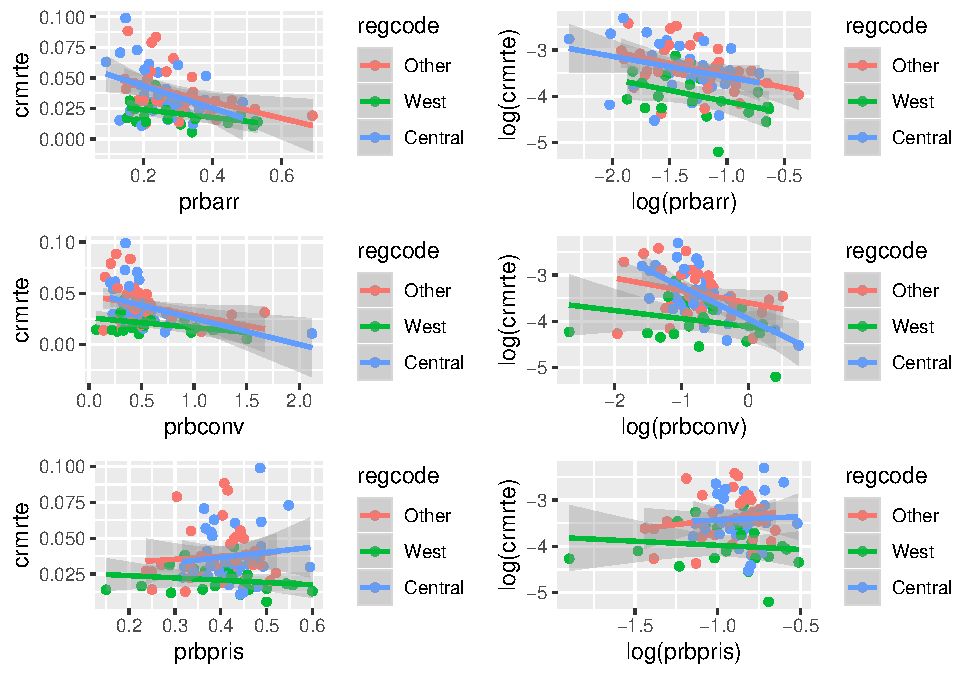
\includegraphics{Bagnard_Gaustad_Hartman_Leung_Lab_3_files/figure-latex/unnamed-chunk-94-1.pdf}

\begin{Shaded}
\begin{Highlighting}[]
\KeywordTok{grid.arrange}\NormalTok{(q4, q4a, q5, q5a, q6, q6a, }\DataTypeTok{ncol=}\DecValTok{2}\NormalTok{)}
\end{Highlighting}
\end{Shaded}

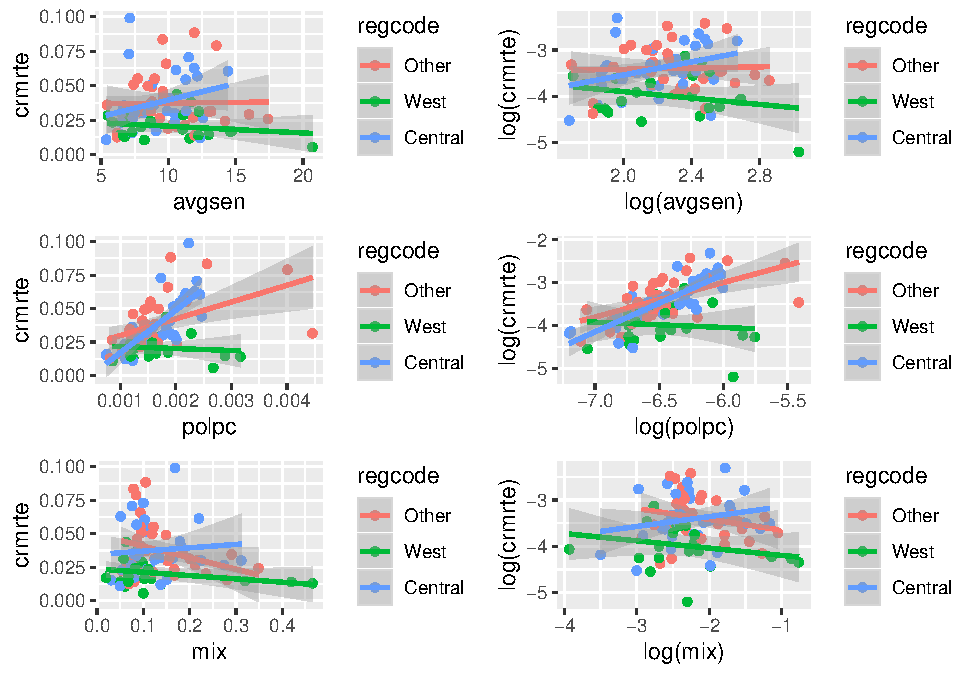
\includegraphics{Bagnard_Gaustad_Hartman_Leung_Lab_3_files/figure-latex/unnamed-chunk-94-2.pdf}

The log transformation for these variables makes the relationship more
linear. We will transform these variables to their log equivalents.

We also note that of the six variables, only prbarr, prbconv and polpc
show univariate correlation with crime. We believe these will be better
candidates for our model selection. Further, we see mix has no
correlation with crmrate and may be its own outcome variable.

\begin{Shaded}
\begin{Highlighting}[]
\NormalTok{dfCrime}\OperatorTok{$}\NormalTok{logprbarr <-}\StringTok{ }\KeywordTok{log}\NormalTok{(dfCrime}\OperatorTok{$}\NormalTok{prbarr)}
\NormalTok{dfCrime}\OperatorTok{$}\NormalTok{logprbconv <-}\StringTok{ }\KeywordTok{log}\NormalTok{(dfCrime}\OperatorTok{$}\NormalTok{prbconv)}
\NormalTok{dfCrime}\OperatorTok{$}\NormalTok{logprbpris <-}\StringTok{ }\KeywordTok{log}\NormalTok{(dfCrime}\OperatorTok{$}\NormalTok{prbpris)}
\NormalTok{dfCrime}\OperatorTok{$}\NormalTok{logavgsen <-}\StringTok{ }\KeywordTok{log}\NormalTok{(dfCrime}\OperatorTok{$}\NormalTok{avgsen)}
\NormalTok{dfCrime}\OperatorTok{$}\NormalTok{logpolpc <-}\StringTok{ }\KeywordTok{log}\NormalTok{(dfCrime}\OperatorTok{$}\NormalTok{polpc)}
\NormalTok{dfCrime}\OperatorTok{$}\NormalTok{logmix <-}\StringTok{ }\KeywordTok{log}\NormalTok{(dfCrime}\OperatorTok{$}\NormalTok{mix)}
\end{Highlighting}
\end{Shaded}

Next we take a look at the demographic variables and their log
alternatives

\begin{Shaded}
\begin{Highlighting}[]
\NormalTok{q1<-}\KeywordTok{ggplot}\NormalTok{(}\DataTypeTok{data =}\NormalTok{ dfCrime, }\KeywordTok{aes}\NormalTok{(}\DataTypeTok{x =}\NormalTok{ pctymle, }\DataTypeTok{y =}\NormalTok{ crmrte, }\DataTypeTok{color =}\NormalTok{ regcode)) }\OperatorTok{+}\StringTok{ }
\StringTok{      }\KeywordTok{geom_point}\NormalTok{()}\OperatorTok{+}
\StringTok{  }\KeywordTok{geom_smooth}\NormalTok{(}\DataTypeTok{method =} \StringTok{"lm"}\NormalTok{)}
\NormalTok{q1a<-}\KeywordTok{ggplot}\NormalTok{(}\DataTypeTok{data =}\NormalTok{ dfCrime, }\KeywordTok{aes}\NormalTok{(}\DataTypeTok{x =} \KeywordTok{log}\NormalTok{(pctymle), }\DataTypeTok{y =} \KeywordTok{log}\NormalTok{(crmrte), }\DataTypeTok{color =}\NormalTok{ regcode)) }\OperatorTok{+}\StringTok{ }
\StringTok{      }\KeywordTok{geom_point}\NormalTok{()}\OperatorTok{+}
\StringTok{  }\KeywordTok{geom_smooth}\NormalTok{(}\DataTypeTok{method =} \StringTok{"lm"}\NormalTok{)}
\NormalTok{q2<-}\KeywordTok{ggplot}\NormalTok{(}\DataTypeTok{data =}\NormalTok{ dfCrime, }\KeywordTok{aes}\NormalTok{(}\DataTypeTok{x =}\NormalTok{ pctmin80, }\DataTypeTok{y =}\NormalTok{ crmrte, }\DataTypeTok{color =}\NormalTok{ regcode)) }\OperatorTok{+}\StringTok{ }
\StringTok{      }\KeywordTok{geom_point}\NormalTok{()}\OperatorTok{+}
\StringTok{  }\KeywordTok{geom_smooth}\NormalTok{(}\DataTypeTok{method =} \StringTok{"lm"}\NormalTok{)}
\NormalTok{q2a<-}\KeywordTok{ggplot}\NormalTok{(}\DataTypeTok{data =}\NormalTok{ dfCrime, }\KeywordTok{aes}\NormalTok{(}\DataTypeTok{x =} \KeywordTok{log}\NormalTok{(pctmin80), }\DataTypeTok{y =} \KeywordTok{log}\NormalTok{(crmrte), }\DataTypeTok{color =}\NormalTok{ regcode)) }\OperatorTok{+}\StringTok{ }
\StringTok{      }\KeywordTok{geom_point}\NormalTok{()}\OperatorTok{+}
\StringTok{  }\KeywordTok{geom_smooth}\NormalTok{(}\DataTypeTok{method =} \StringTok{"lm"}\NormalTok{)}
\NormalTok{q3<-}\KeywordTok{ggplot}\NormalTok{(}\DataTypeTok{data =}\NormalTok{ dfCrime, }\KeywordTok{aes}\NormalTok{(}\DataTypeTok{x =}\NormalTok{ density, }\DataTypeTok{y =}\NormalTok{ crmrte, }\DataTypeTok{color =}\NormalTok{ regcode)) }\OperatorTok{+}\StringTok{ }
\StringTok{      }\KeywordTok{geom_point}\NormalTok{()}\OperatorTok{+}
\StringTok{  }\KeywordTok{geom_smooth}\NormalTok{(}\DataTypeTok{method =} \StringTok{"lm"}\NormalTok{)}
\NormalTok{q3a<-}\KeywordTok{ggplot}\NormalTok{(}\DataTypeTok{data =}\NormalTok{ dfCrime, }\KeywordTok{aes}\NormalTok{(}\DataTypeTok{x =} \KeywordTok{log}\NormalTok{(density), }\DataTypeTok{y =} \KeywordTok{log}\NormalTok{(crmrte), }\DataTypeTok{color =}\NormalTok{ regcode)) }\OperatorTok{+}\StringTok{ }
\StringTok{      }\KeywordTok{geom_point}\NormalTok{()}\OperatorTok{+}
\StringTok{  }\KeywordTok{geom_smooth}\NormalTok{(}\DataTypeTok{method =} \StringTok{"lm"}\NormalTok{)}


\KeywordTok{grid.arrange}\NormalTok{(q1, q1a, q2, q2a, q3, q3a, }\DataTypeTok{ncol=}\DecValTok{2}\NormalTok{)}
\end{Highlighting}
\end{Shaded}

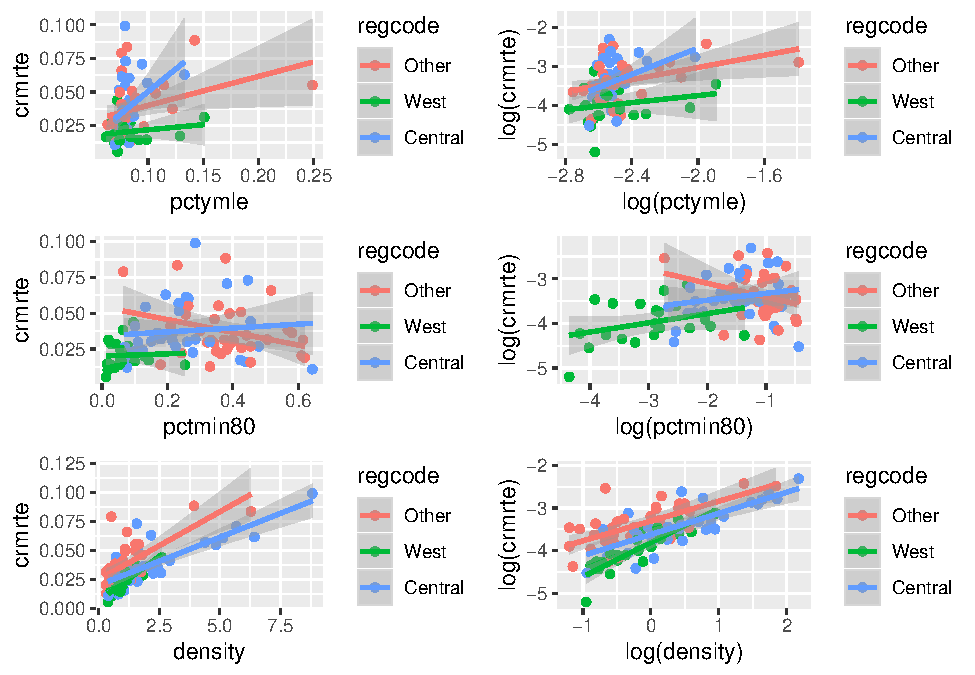
\includegraphics{Bagnard_Gaustad_Hartman_Leung_Lab_3_files/figure-latex/unnamed-chunk-96-1.pdf}

Again we see improvements after transformation. We will include
transforms of these variables as well.

\begin{Shaded}
\begin{Highlighting}[]
\NormalTok{dfCrime}\OperatorTok{$}\NormalTok{logdensity <-}\StringTok{ }\KeywordTok{log}\NormalTok{(dfCrime}\OperatorTok{$}\NormalTok{density)}
\NormalTok{dfCrime}\OperatorTok{$}\NormalTok{logpctmin80 <-}\StringTok{ }\KeywordTok{log}\NormalTok{(dfCrime}\OperatorTok{$}\NormalTok{pctmin80)}
\NormalTok{dfCrime}\OperatorTok{$}\NormalTok{logpctymle <-}\StringTok{ }\KeywordTok{log}\NormalTok{(dfCrime}\OperatorTok{$}\NormalTok{pctymle)}
\end{Highlighting}
\end{Shaded}

Finally, we'll take a look at taxpc and a histogram of the crmrte
variable itself.

\begin{Shaded}
\begin{Highlighting}[]
\NormalTok{q1<-}\KeywordTok{ggplot}\NormalTok{(}\DataTypeTok{data =}\NormalTok{ dfCrime, }\KeywordTok{aes}\NormalTok{(}\DataTypeTok{x =}\NormalTok{ taxpc, }\DataTypeTok{y =}\NormalTok{ crmrte, }\DataTypeTok{color =}\NormalTok{ regcode)) }\OperatorTok{+}\StringTok{ }
\StringTok{      }\KeywordTok{geom_point}\NormalTok{()}\OperatorTok{+}
\StringTok{  }\KeywordTok{geom_smooth}\NormalTok{(}\DataTypeTok{method =} \StringTok{"lm"}\NormalTok{)}
\NormalTok{q1a<-}\KeywordTok{ggplot}\NormalTok{(}\DataTypeTok{data =}\NormalTok{ dfCrime, }\KeywordTok{aes}\NormalTok{(}\DataTypeTok{x =} \KeywordTok{log}\NormalTok{(taxpc), }\DataTypeTok{y =} \KeywordTok{log}\NormalTok{(crmrte), }\DataTypeTok{color =}\NormalTok{ regcode)) }\OperatorTok{+}\StringTok{ }
\StringTok{      }\KeywordTok{geom_point}\NormalTok{()}\OperatorTok{+}
\StringTok{  }\KeywordTok{geom_smooth}\NormalTok{(}\DataTypeTok{method =} \StringTok{"lm"}\NormalTok{)}

\NormalTok{q2<-}\KeywordTok{ggplot}\NormalTok{(}\DataTypeTok{data =}\NormalTok{ dfCrime, }\KeywordTok{aes}\NormalTok{(}\DataTypeTok{x =}\NormalTok{ crmrte)) }\OperatorTok{+}\StringTok{ }
\StringTok{      }\KeywordTok{geom_histogram}\NormalTok{(}\DataTypeTok{bins=}\DecValTok{30}\NormalTok{)}
\NormalTok{q2a<-}\KeywordTok{ggplot}\NormalTok{(}\DataTypeTok{data =}\NormalTok{ dfCrime, }\KeywordTok{aes}\NormalTok{(}\DataTypeTok{x =} \KeywordTok{log}\NormalTok{(crmrte))) }\OperatorTok{+}\StringTok{ }
\StringTok{      }\KeywordTok{geom_histogram}\NormalTok{(}\DataTypeTok{bins=}\DecValTok{30}\NormalTok{)}

\KeywordTok{grid.arrange}\NormalTok{(q1, q1a, q2, q2a, }\DataTypeTok{ncol=}\DecValTok{2}\NormalTok{)}
\end{Highlighting}
\end{Shaded}

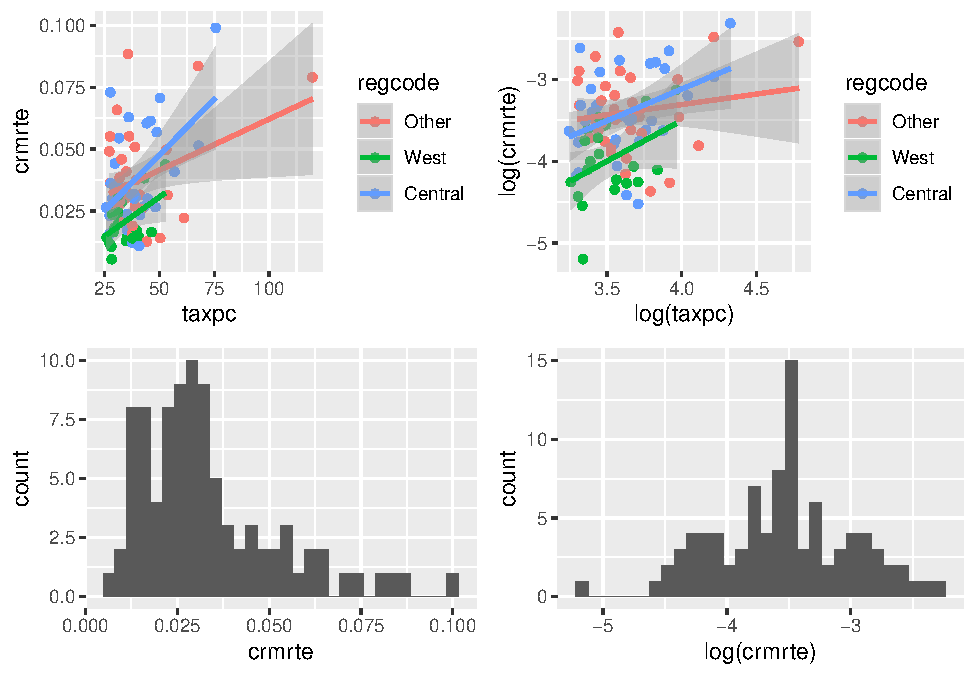
\includegraphics{Bagnard_Gaustad_Hartman_Leung_Lab_3_files/figure-latex/unnamed-chunk-98-1.pdf}

The crmrte and taxpc variables also show improvement after
transformation. We'll add those to our dataframe.

\begin{Shaded}
\begin{Highlighting}[]
\NormalTok{dfCrime}\OperatorTok{$}\NormalTok{logcrmrte =}\StringTok{ }\KeywordTok{log}\NormalTok{(dfCrime}\OperatorTok{$}\NormalTok{crmrte)}
\NormalTok{dfCrime}\OperatorTok{$}\NormalTok{logtaxpc =}\StringTok{ }\KeywordTok{log}\NormalTok{(dfCrime}\OperatorTok{$}\NormalTok{taxpc)}
\end{Highlighting}
\end{Shaded}


\end{document}
